\documentclass[english,letter paper,12pt,leqno]{article}
\usepackage{stmaryrd}
\usepackage{amsmath, amscd, amssymb, mathrsfs, accents, amsfonts,amsthm}
\usepackage[all]{xy}
\usepackage{dsfont}
\usepackage{tikz}
\def\nicedashedcolourscheme{\shadedraw[top color=blue!22, bottom color=blue!22, draw=gray, dashed]}
\def\nicecolourscheme{\shadedraw[top color=blue!22, bottom color=blue!22, draw=white]}
\def\nicepalecolourscheme{\shadedraw[top color=blue!12, bottom color=blue!12, draw=white]}
\def\nicenocolourscheme{\shadedraw[top color=gray!2, bottom color=gray!25, draw=white]}
\def\nicereallynocolourscheme{\shadedraw[top color=white!2, bottom color=white!25, draw=white]}
\definecolor{Myblue}{rgb}{0,0,0.6}
\usepackage[a4paper,colorlinks,citecolor=Myblue,linkcolor=Myblue,urlcolor=Myblue,pdfpagemode=None]{hyperref}

\SelectTips{cm}{}

\setlength{\evensidemargin}{0.1in}
\setlength{\oddsidemargin}{0.1in}
\setlength{\textwidth}{6.3in}
\setlength{\topmargin}{0.0in}
\setlength{\textheight}{8.5in}
\setlength{\headheight}{0in}

\newtheorem{theorem}{Theorem}[section]
\newtheorem{proposition}[theorem]{Proposition}
\newtheorem{lemma}[theorem]{Lemma}
\newtheorem{corollary}[theorem]{Corollary}
\newtheorem{setup}[theorem]{Setup}

\newtheoremstyle{example}{\topsep}{\topsep}
	{}
	{}
	{\bfseries}
	{.}
	{2pt}
	{\thmname{#1}\thmnumber{ #2}\thmnote{ #3}}
	
	\theoremstyle{example}
	\newtheorem{definition}[theorem]{Definition}
	\newtheorem{example}[theorem]{Example}
	\newtheorem{remark}[theorem]{Remark}
	\newtheorem{strat}[theorem]{Strategy}

\numberwithin{equation}{section}

% Operators
\def\eval{\operatorname{ev}}
\def\res{\operatorname{Res}}
\def\Coker{\operatorname{Coker}}
\def\Ker{\operatorname{Ker}}
\def\im{\operatorname{Im}}
\def\can{\operatorname{can}}
\def\K{\mathbf{K}}
\def\D{\mathbf{D}}
\def\N{\mathbf{N}}
\def\LG{\mathcal{LG}}
\def\Ab{\operatorname{Ab}}
\def\stab{\operatorname{stab}}
\def\Hom{\operatorname{Hom}}
\def\modd{\operatorname{mod}}
\def\Modd{\operatorname{Mod}}
\def\be{\begin{equation}}
\def\ee{\end{equation}}
\def\nN{\mathds{N}}
\def\nZ{\mathds{Z}}
\def\nQ{\mathds{Q}}
\def\nR{\mathds{R}}
\def\nC{\mathds{C}}
\DeclareMathOperator{\Ext}{Ext}
\DeclareMathOperator{\Tr}{Tr}
\DeclareMathOperator{\End}{End}
\DeclareMathOperator{\rank}{rank}
\DeclareMathOperator{\tot}{Tot}
\DeclareMathOperator{\ch}{ch}
\DeclareMathOperator{\str}{str}
\DeclareMathOperator{\hmf}{hmf}
\DeclareMathOperator{\HMF}{HMF}
\DeclareMathOperator{\hf}{HF}
\DeclareMathOperator{\At}{At}
\DeclareMathOperator{\Cat}{Cat}
\DeclareMathOperator{\Spec}{Spec}

\begin{document}

% Commands
\def\Res{\res\!}
\newcommand{\ud}{\mathrm{d}}
\newcommand{\Ress}[1]{\res_{#1}\!}
\newcommand{\cat}[1]{\mathcal{#1}}
\newcommand{\lto}{\longrightarrow}
\newcommand{\xlto}[1]{\stackrel{#1}\lto}
\newcommand{\mf}[1]{\mathfrak{#1}}
\newcommand{\md}[1]{\mathscr{#1}}
\def\sus{\l}
\def\l{\,|\,}
\def\sgn{\textup{sgn}}

\title{$A_\infty$-minimal models of matrix factorisations}
\author{Daniel Murfet}

\maketitle


\section{Generator cuts}

\begin{remark} For example in Example \ref{example:stabkpre} the only interaction that can remove a $\theta_k$ particle is (C.2), and the only interaction that removes an $x_k$ is (B). Thus every occurrence of an $(\textup{A}.4)_{i=1,k=1,\delta=(2,0)}$ interaction in a Feynman diagram for $W = x_2^3 - x_1^3$ with nonzero contribution needs to be accompanied (further down the tree) by both a $(\textup{C}.2)_{j=1}$ for $\theta_1$ and a $(\textup{B})_{k = 1}$ for the $x_1$, which in turn requires its own $(\textup{C}.2)_{j=1}$ even further down the tree.
\end{remark}

We can depict a series of choices by linking the creation and annihilation operators,
\begin{center}
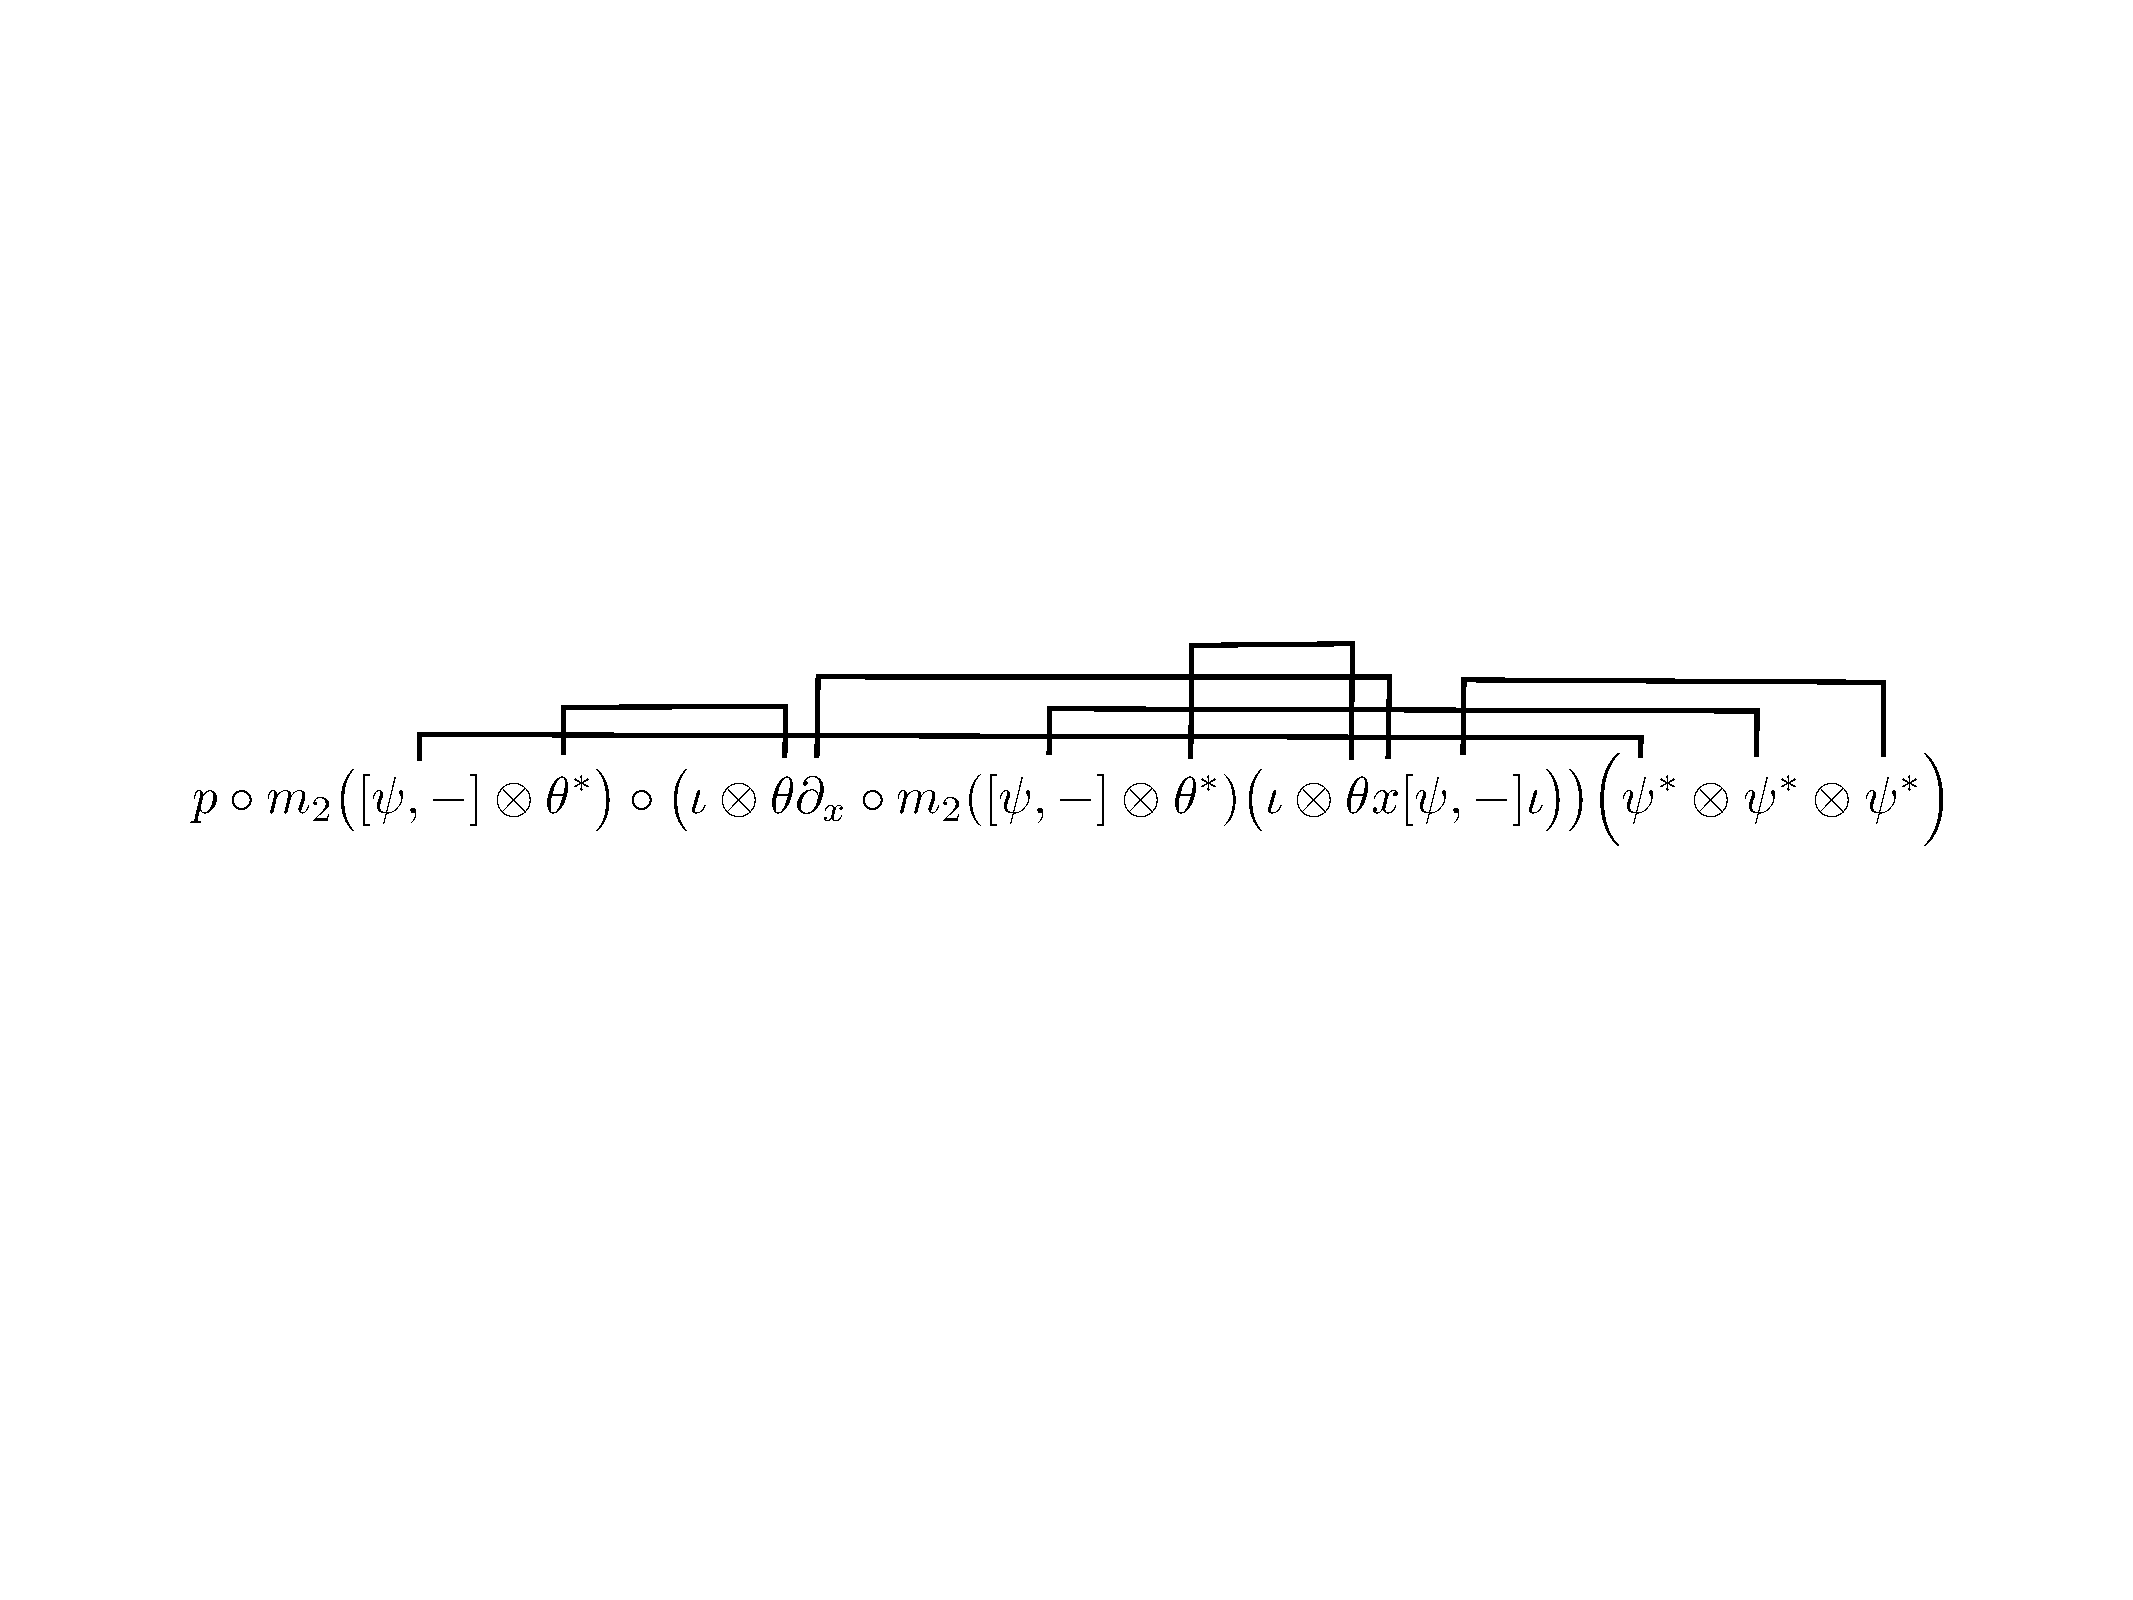
\includegraphics[scale=0.45]{dia8}
\end{center}
or by drawing these linkages, marked with the type and index of the ``particle'' on the tree $T$, joining the two positions determined by the configuration as in Example \ref{ex:picture_example}.

\begin{example}\label{example:stabkpre} Let $k$ be a field, set $\mathfrak{m} = (x_1,\ldots,x_n) \subseteq R$ and suppose that $W \in \mathfrak{m}^3$ (we address the case where $W$ has quadratic factors separately below). From any choice of a presentation $W = \sum_{i=1}^n x_i W^i$ with $W^i \in \mathfrak{m}^2$ we obtain a Koszul matrix factorisation
\begin{equation}\label{eq:kstab}
k^{\operatorname{stab}} = \Big( \bigwedge F_\xi \otimes R, \;d_{k^{\stab}} = \sum_{i=1}^n x_i \xi_i^* + \sum_{i=1}^n W^i \xi_i \Big)
\end{equation}
referred to as the \emph{stabilisation} of the residue field $k = R / \mathfrak{m}$ see \cite{??}. We set $X = Y = k^{\stab}$ but write as above $\eta_1,\ldots,\eta_n$ for the copies of the generators $\xi_i$ belonging to the $Y$ copy of $k^{\stab}$, and we write $\psi_i = \xi_i^*$ as above. The state spaces associated to the boundary and interior of the trees are therefore respectively
\begin{align*}
\KK &= \bigwedge F_\xi \otimes \bigwedge F_\xi^*\,, \qquad \HH = \bigwedge \big( F_\theta \oplus F_\xi \oplus F_\xi^* \big) \otimes k\llbracket \bold{x} \rrbracket\,.
\end{align*}
Then $f_i = u_i = x_i$ and $g_i = v_i = W^i$ for $1 \le i \le n$. In Setup \ref{setup:overall} we take
\[
\bold{t} = (x_1,\ldots,x_n)\,, \qquad \lambda_k = \eta_k \wedge (-)
\]
with $\sigma: k \lto R$ the inclusion of the constants, so $\partial_{t_i} = \partial_{x_i}$, and the homotopy $\lambda_k$ being the wedge product on the left with $\eta_k$. For $r \in R$ the coefficient $r_{(1,\alpha)}$ is just the coefficient $r_\alpha$ of the monomial $x^\alpha$ in $R$, so that $(F_{kj})_{(1,\alpha)} = 0, \Gamma^{mh}_{l \beta} = \delta_{\beta = \bold{0}}$ and
\begin{align*}
(f_j)_{(1,\alpha)} &= (u_j)_{(1,\alpha)} = (x_j)_{(1,\alpha)} = \delta_{\alpha = \bold{e}_j}\\
(g_j)_{(1,\alpha)} &= (v_j)_{(1,\alpha)} = (W^j)_{(1,\alpha)} = W^j_{\alpha}\\
(G_{kj})_{(1,\alpha)} &= (\delta_{k=j})_{(1,\alpha)} = \delta_{k=j} \delta_{\alpha = \bold{0}}
\end{align*}
We may omit the $R/I = k$ lines from the Feynman diagrams. 
%\begin{center}
%\begin{tabular}{ >{\centering}m{5cm} >{\centering}m{5cm} >{\centering}m{5cm} }
%\textbf{(A.1)}
%\\
%\[
%\xymatrix@C+2pc@R+1pc{
%& \ar@{-}[d]^-{\eta_j}\\
%& \bullet \ar@{=}[d]^-{\theta_j}\\
%& &
%}
%\]
%&
%\textbf{(C.2)}
%\\
%\[
%\xymatrix@C+2pc@R+1pc{
%&  \ar@{=}[d]^-{\theta_j} \\
%& \bullet \ar@{-}[d]^-{\eta_j}\\
%& &
%}
%\]
%&
%\textbf{(B)}
%\\
%\[
%\xymatrix@R+1pc{
%\ar@{~}[d]^-{x_k}\\
%\bullet \ar@{=}[d]^-{\theta_k}\\
%\;
%}
%\]
%\end{tabular}
%\end{center}

%\begin{center}
%\begin{tabular}{ >{\centering}m{8cm} >{\centering}m{6cm} }
%\[
%\xymatrix@C+1pc@R+3pc{
%& & \bullet \ar@{=}[dll]_-{\theta_k} \ar@{~}[d]_-{\partial_{x_k}(x^\delta)} %\ar@{-}[drr]^-{\eta_j}\\
%& & & &
%}
%\]
%&
%\textbf{(A.2)}
%\vspace{1cm}
%\[ W^j_\delta \]
%\end{tabular}
%\end{center}

%\begin{center}
%\begin{tabular}{ >{\centering}m{8cm} >{\centering}m{6cm} }
%\[
%\xymatrix@C+2pc@R+2pc{
%& \bullet \ar@{=}[dl]_-{\theta_i} \ar@{-}[dr]^-{\psi_i}\\
%& &
%}
%\]
%&
%\textbf{(A.3)}
%\vspace{1cm}
%\[ -1 \]
%\end{tabular}
%\end{center}

%\begin{center}
%\begin{tabular}{ >{\centering}m{8cm} >{\centering}m{6cm} }
%\[
%\xymatrix@C+2pc@R+2pc{
%& \ar@{-}[d]^-{\psi_i}\\
%& \bullet \ar@{=}[dl]^-{\theta_k} \ar@{~}[dr]^-{\partial_{x_k}(x^\delta)}\\
%& &
%}
%\]
%&
%\textbf{(A.4)}
%\vspace{1cm}
%\[ W^i_\delta \]
%\end{tabular}
%\end{center}
%As it turns out, the best way to understand the $A_\infty$-products in this case is to organise the interactions a little differently, see Section \ref{??}. 

For concreteness, we remark that if $n = 2$ and $W = x_2^3 - x_1^3$ then we may choose $W^1 = -x_1^2, W^2 = x_2^2$ and so there are two (A.4) type interactions, respectively
\begin{center}
\begin{tabular}{ >{\centering}m{8cm} >{\centering}m{6cm} }
\[
\xymatrix@C+2pc@R+2pc{
& \ar@{-}[d]^-{\psi_1}\\
& \bullet \ar@{=}[dl]^-{\theta_1} \ar@{~}[dr]^-{\partial_{x_1}(x_1^2) = 2x}\\
& &
}
\]
&
\textbf{(A.4)}$_{i=1,k=1,\delta=(2,0)}$
\vspace{1cm}
\[ W^1_{(2,0)} = -1 \]
\end{tabular}
\end{center}
and the other similar diagram involving $\psi_2, \theta_2, \partial_{x_2}(x_2^2)$ and a coefficient $W^2_{(0,2)} = 1$. 
\end{example}

Suppose that $k$ is a field and that the potential $W$ belongs to $\mathfrak{m}^3$ where $\mathfrak{m} = (x_1,\ldots,x_n)$, choose a presentation $W = \sum_i x_i W^i$ with $W^i \in \mathfrak{m}^2$ and consider the following pair
\begin{equation}\label{eq:kstab}
k^{\operatorname{stab}} = \Big( k[x] \otimes \bigwedge\big( \oplus_{i=1}^n k\psi_i \,\big), \;d_{k^{\stab}} = \sum_{i=1}^n x_i \psi_i^* + \sum_{i=1}^n W^i \psi_i \Big)
\end{equation}
where $\psi_i^*, \psi_i$ denote respectively the operators of contraction $\psi_i^* \lrcorner (-)$ and wedge product $\psi_i = \psi_i \wedge (-)$ on the exterior algebra. Clearly $(d_{k^{\stab}})^2 = W$ so that $k^{\stab}$ is a matrix factorisation of $W$. When $k$ is a field and $W$ has an isolated critical point at the origin, $k^{\stab}$ is the representative in the homotopy category of matrix factorisations of the structure sheaf of the singular point at the origin, and was first studied by Dyckerhoff \cite{d0904.4713}. If the origin is the only singular point of the zero locus of $W$, or we work with power series instead of the polynomial ring, $k^{\stab}$ is a split generator of the homotopy category of matrix factorisations \cite[Theorem ?]{?}.

\begin{remark} This can alternatively be done by perturbation on the underlying complex of the generator.
\end{remark}

The purpose of this paper is to show how to calculate the $A_\infty$-minimal model $\mathscr{B}$ of the $\nZ_2$-graded differential graded endomorphism algebra
\be\label{eq:defnaw}
\mathscr{A} = \Big( \End_{k[x]}(k^{\operatorname{stab}}), \; \partial = [d_{k^{\stab}},-] \; \Big)\,.
\ee 
The differential here is (throughout all commutators are graded commutators)
\begin{align*}
\partial = [d_{k^{\stab}},-] &= \Big[\sum_i x_i \psi_i^* + \sum_i W^i \psi_i, -\Big]\\
&= \sum_i x_i [\psi_i^*,-] + \sum_i W^i [\psi_i,-]\,.
\end{align*}
The minimal model is a finite-dimensional $\nZ_2$-graded vector space $\mathscr{B}$ with a family 
\[
\left\{ \rho_q: \big(\mathscr{B}[1]\big)^{\otimes q} \lto \mathscr{B}[1] \right\}_{q \ge 2}
\]
of odd $k$-linear maps satisfying the forward suspended $A_\infty$-constraints \cite{lazaroiu}, and having the property that there is an $A_\infty$-quasi-isomorphism $\mathscr{B} \lto \mathscr{A}$.

The $A_\infty$-products on $\mathscr{B}$ are defined in terms of Feynman diagrams (see Definition \ref{defn:bainf}). In this section we explain how to enumerate all the relevant diagrams and how to compute their value; in the next section we prove that the maps they give rise to do indeed compute the minimal model of $\mathscr{A}$. 

Throughout $\otimes = \otimes$. The integer $n$ is the number of variables in the ambient ring $R = k[x_1,\ldots,x_n]$. We assume in this section that $W \in \mathfrak{m}^3$. This is not a real restriction, as we will prove in Section \ref{??} that if $W \in \mathfrak{m}^2$ is written in the form
\be
W = W'(x_1,\ldots,x_r) + \sum_{i={r+1}}^n \lambda_i x_i^2\,, \quad \text{ with } \quad W' \in \mathfrak{m}^3
\ee
and if $\mathscr{B}'$ denotes the minimal model of $W'$ as constructed below, then as $A_\infty$-algebras
\be
\mathscr{B} \cong \mathscr{B}' \otimes C( Q )
\ee
where $C(Q)$ is the Clifford algebra of the quadratic form $Q = \sum_{i=r+1}^n \lambda_i x_i^2$, with no higher products (i.e. viewed simply as a $\nZ_2$-graded algebra). We may therefore restrict without loss of generality to $W \in \mathfrak{m}^3$ in what follows.

\begin{definition}\label{defn:handop} Consider the $\nZ_2$-graded $k$-algebra defined by the tensor product
\be
\HH = R \otimes \bigwedge\big( \oplus_{i=1}^n k \theta_i \,\big) \otimes \End_k\Big( \bigwedge\big( \oplus_{i=1}^n k \psi_i \, \big) \Big)
\ee
with degrees $|x_i| = 0$ and $|\theta_i| = |\psi_i| = 1$. On this space we have homogeneous operators
\be
x_i\,, \partial_i = \partial_{x_i}\,, \theta_i\,, \theta_i^*\,, \big[\psi_i\,,-\big]\,.
\ee
Here $\psi_i$ denotes the operator $\psi_i \wedge (-)$ on $\bigwedge\big( \oplus_{i=1}^n k \psi_i \, \big)$ and $[ \psi_i, - ]$ the graded commutator with this operator, defined on a homogeneous operator $\beta$ by
\[
\big[ \psi_i, \beta \big] = \psi_i \circ \beta - (-1)^{|\beta|} \beta \circ \psi_i\,.
\]
We define the $\nZ_2$-graded $k$-module
\be\label{defn:B}
\mathscr{B} = \bigwedge\big( \oplus_{i=1}^n k \psi_i^* \,\big)
\ee
with $|\psi_i^*| = 1$ which we view as a graded submodule
\[
\mathscr{B} \subset \End_k\Big( \bigwedge\big( \oplus_{i=1}^n k \psi_i \, \big) \Big)
\]
by identifying $\psi_i^* \in \mathscr{B}$ with the operation of contraction $\psi_i^*\, \lrcorner\, (-)$ on the exterior algebra. In this way we may also identify $\mathscr{B}$ with a submodule of $\HH$, and we write $\sigma: \mathscr{B} \lto \HH$ for the inclusion. Note that the operator $[\psi_j, -]$ on $\HH$ defined above acts on the submodule $\mathscr{B}$ as contraction with $\psi_j = (\psi_j^*)^*$, that is,
\be\label{eq:comm_is_ann}
\Big[ \psi_j, \sigma\big(\psi_{i_1}^* \wedge \cdots \wedge \psi_{i_r}^*\big) \Big] = \sum_{l=1}^r (-1)^{l-1} \delta_{j, i_l} \sigma\big(\psi_{i_1}^* \wedge \cdots \wedge \widehat{ \psi_{i_l}^* } \wedge \cdots \wedge \psi_{i_r}^*\big)\,.
\ee
We write $p: \HH \lto \HH$ for the $k$-algebra endomorphism of $\HH$ sending $x_i, \theta_i$ to zero for $1 \le i \le n$ and which is the identity on $\End_k( \wedge( \oplus_i k\psi_i ) )$.
\end{definition}

We view $\HH$ as the tensor product of the bosonic Fock space $R$ with creation and annihilation operators $x_i, \partial_i$, fermionic Fock space $\wedge( \oplus_{i=1}^n k \theta_i )$ with creation and annihilation operators $\theta_i, \theta_i^*$ and the third factor, of which the calculations of the $A_\infty$-structure only involve the submodule $\mathscr{B} = \wedge( \oplus_{i=1}^n k \psi_i^* )$ which is another fermionic Fock space. The inputs to the Feynman diagrams are tensor products of states in $\mathscr{B}$, that is, wedge products of $\psi_i^*$'s, on which the $[\psi_i, -]$ act as annihilation operators.

The linear maps in \eqref{eq:int_input}, \eqref{eq:int_intedge}, \eqref{eq:int_intvert} below which determine the $A_\infty$ products $\rho_q$ on $\mathscr{B}$ will be defined in terms of these creation and annihilation operators on $\HH$, and may be interpreted as particle interactions in the usual way. The interactions that appear are the following ones, depicted on the left as Feynman diagrams and on the right as operators. We call these respectively \emph{A-, B- and C-type interactions}:

\begin{center}
\begin{tabular}{ >{\centering}m{1cm} >{\centering}m{4cm} >{\centering}m{8cm} >{\centering}m{1cm}}
\textbf{A}
&
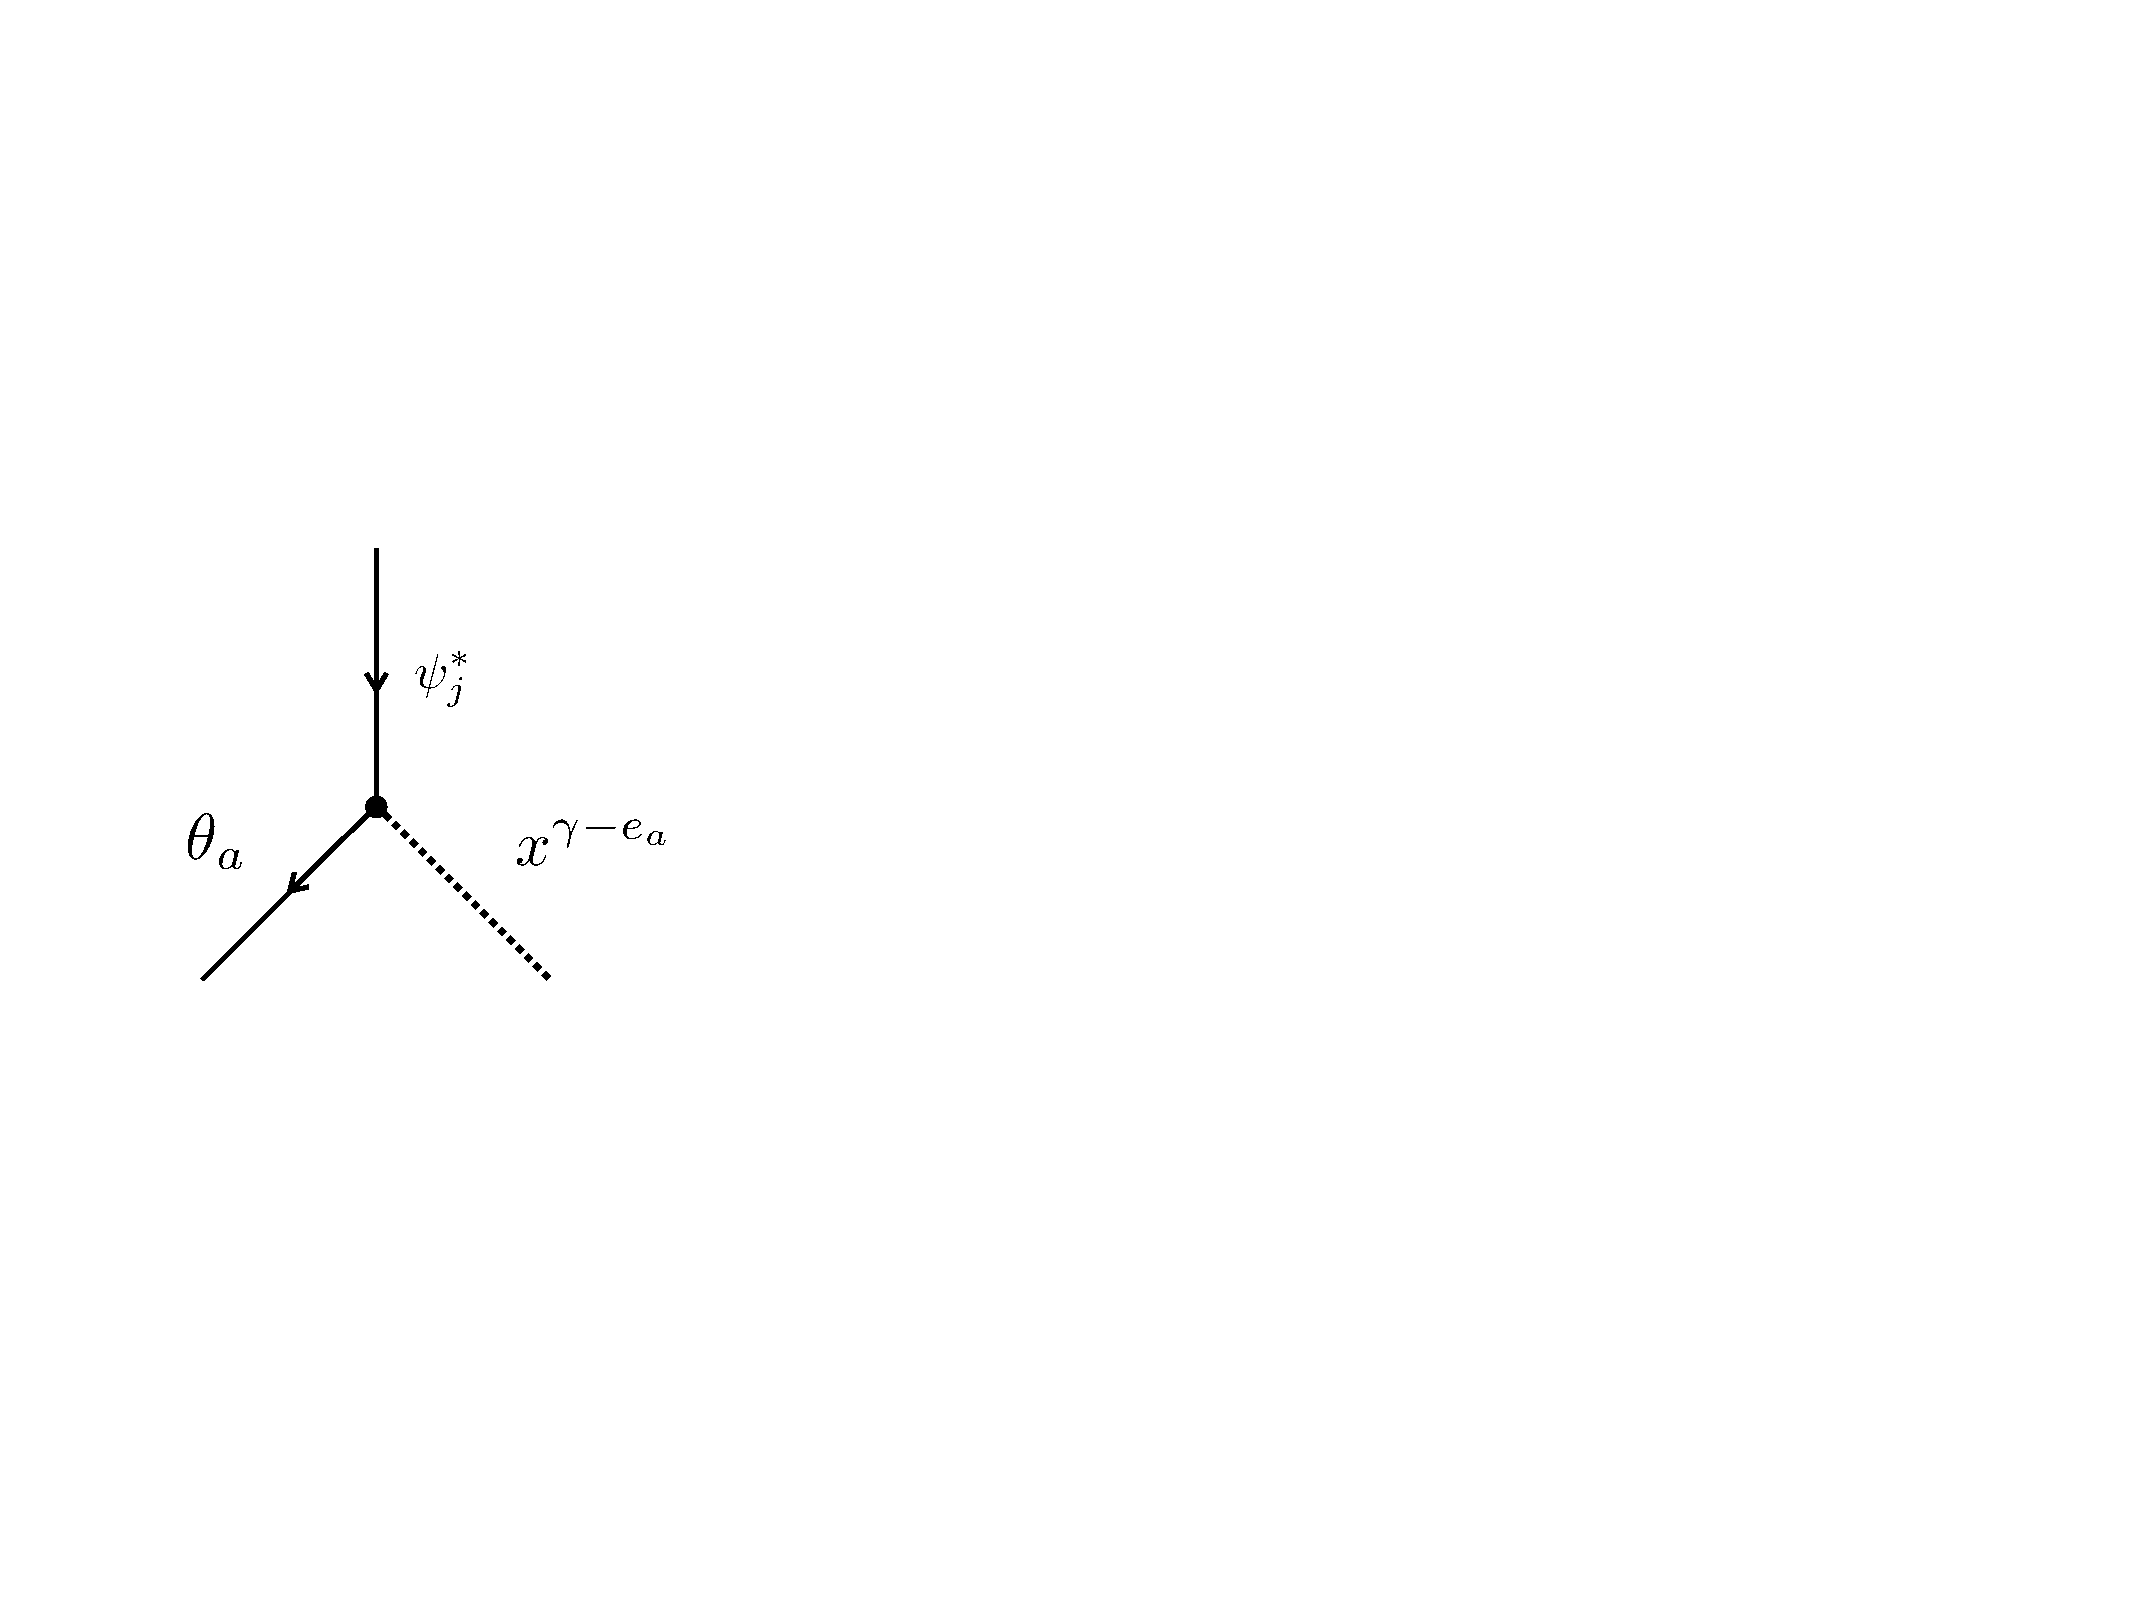
\includegraphics[scale=0.4]{dia2}
&
$\theta_a x^{\gamma - e_a} \big[\psi_j, -\big] \in \End_k( \HH )$\\
\vspace{0.5cm}
$1 \le a,j \le n\,, \gamma \in \mathbb{N}^n$
&
\tagarray{\label{interaction_1}}
\end{tabular}
\end{center}

\begin{center}
\begin{tabular}{ >{\centering}m{1cm} >{\centering}m{4cm} >{\centering}m{8cm} >{\centering}m{1cm}}
\textbf{B}
&
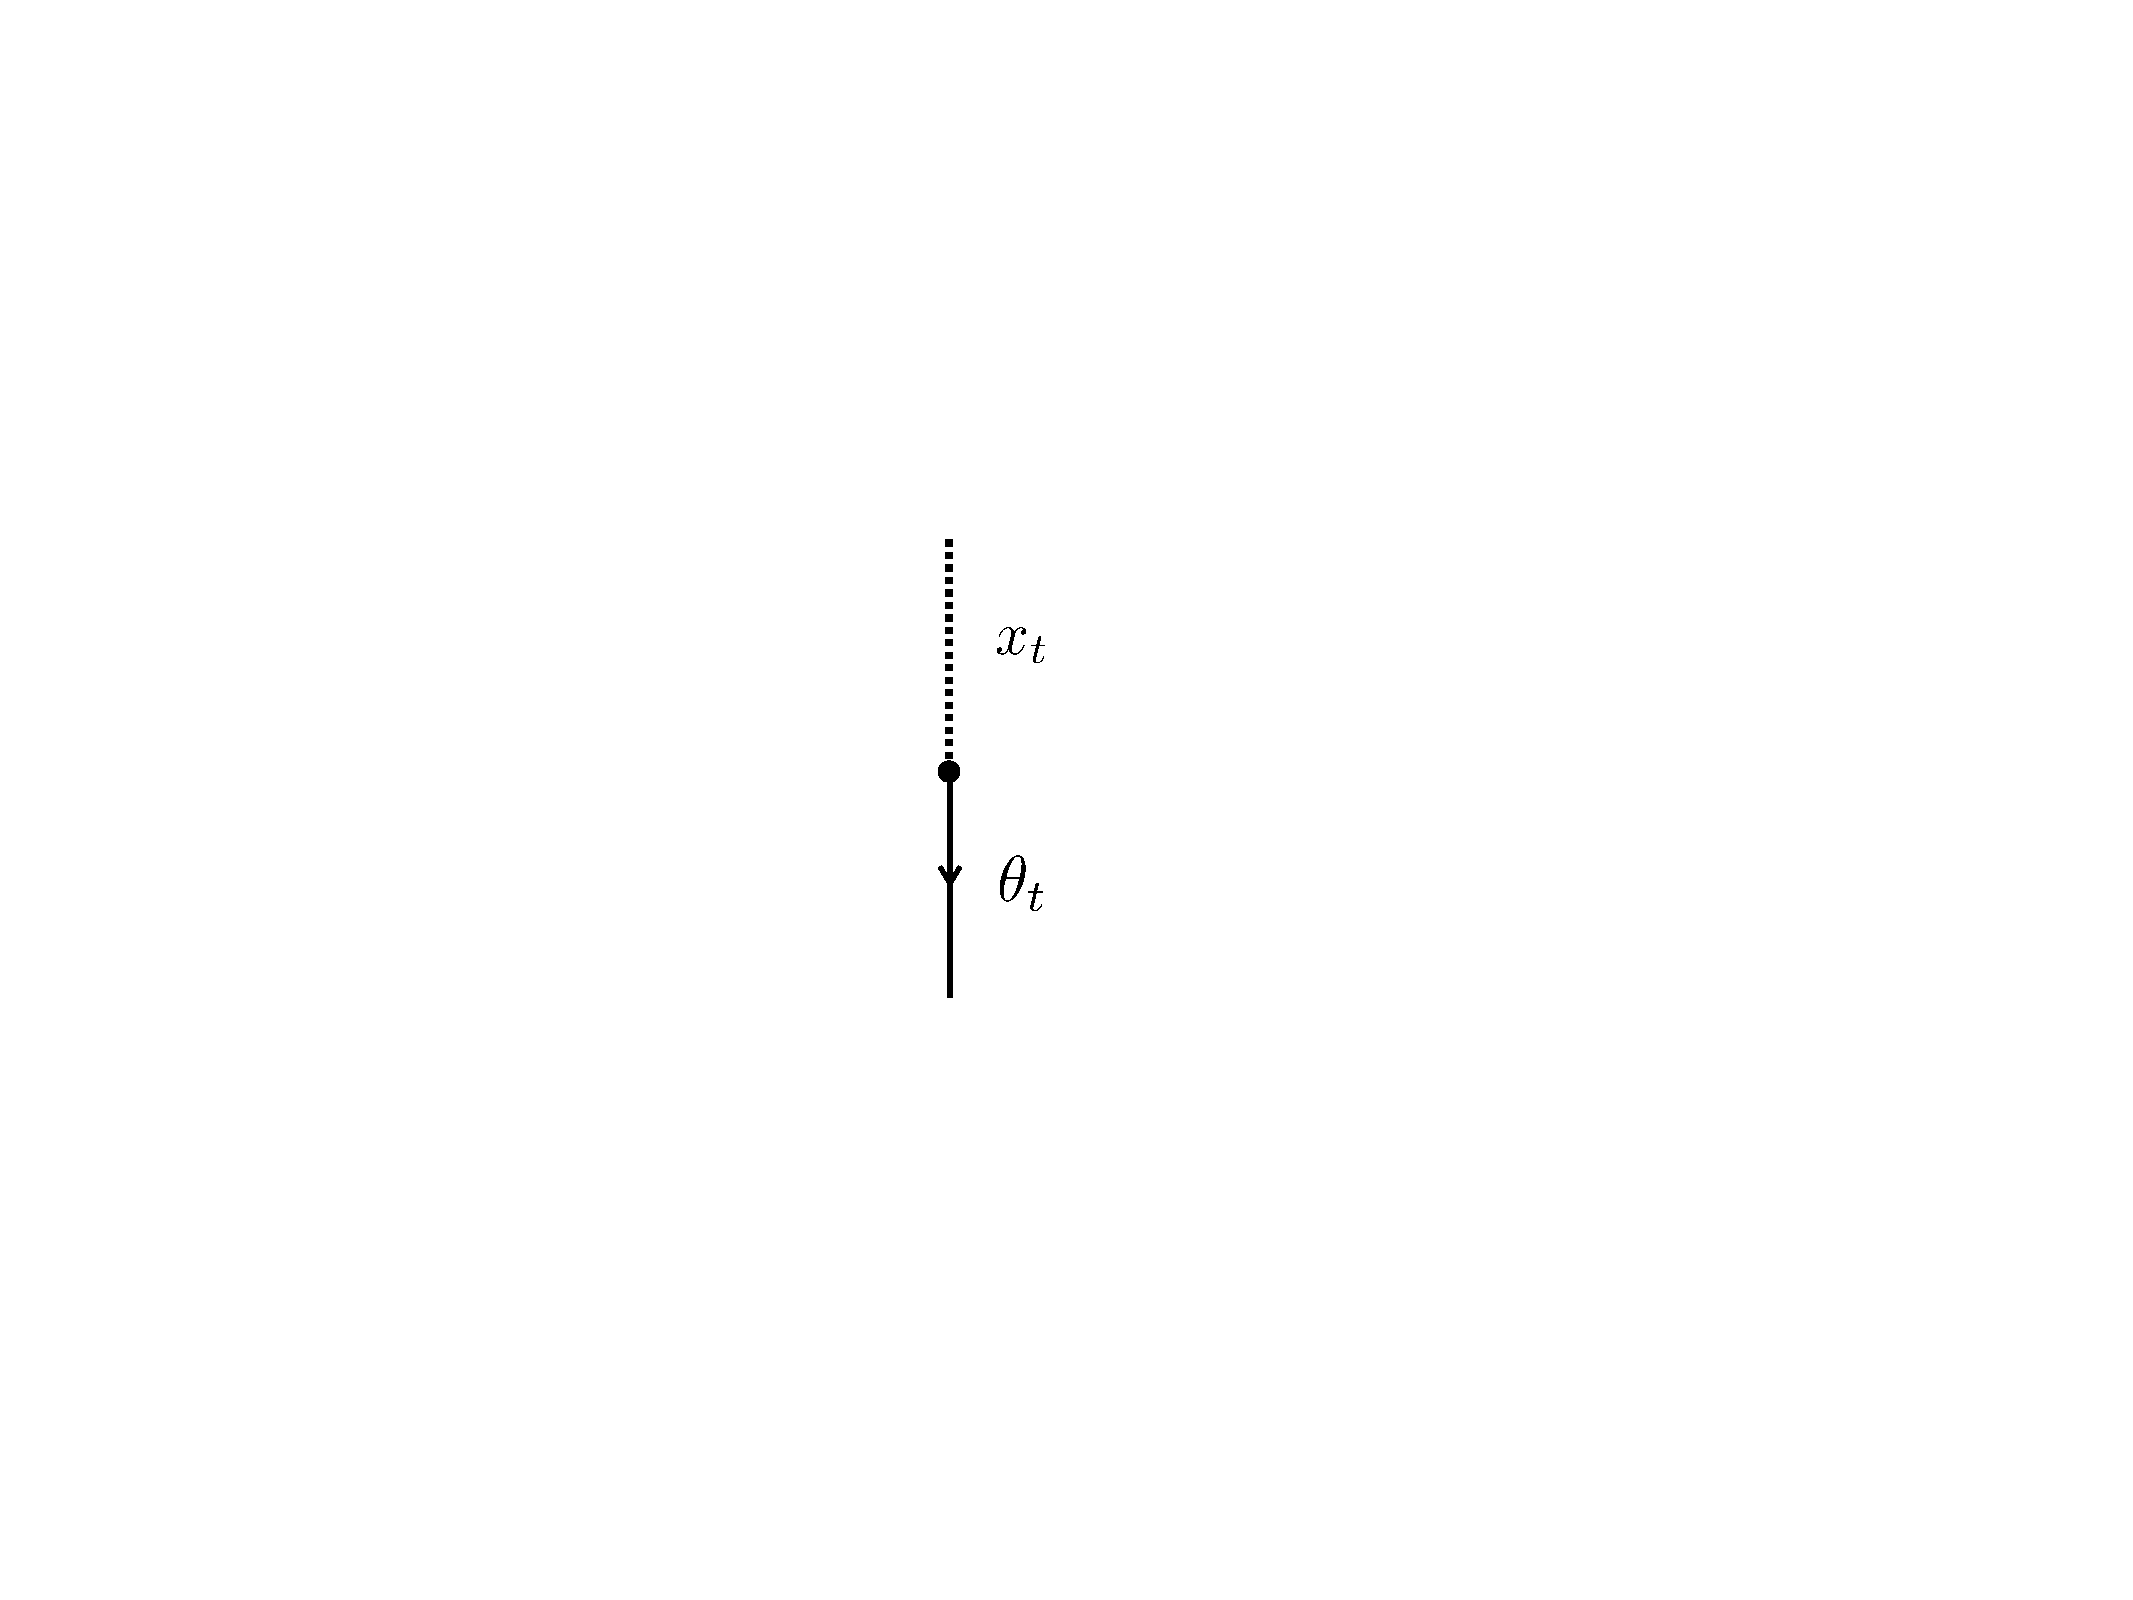
\includegraphics[scale=0.4]{dia3}
&
$\theta_t \partial_t \in \End_k( \HH )$\\
\vspace{0.5cm}
$1 \le t \le n$
&
\tagarray{\label{interaction_2}}
\end{tabular}
\end{center}

\begin{center}
\begin{tabular}{ >{\centering}m{1cm} >{\centering}m{4cm} >{\centering}m{8cm} >{\centering}m{1cm}}
\textbf{C}
&
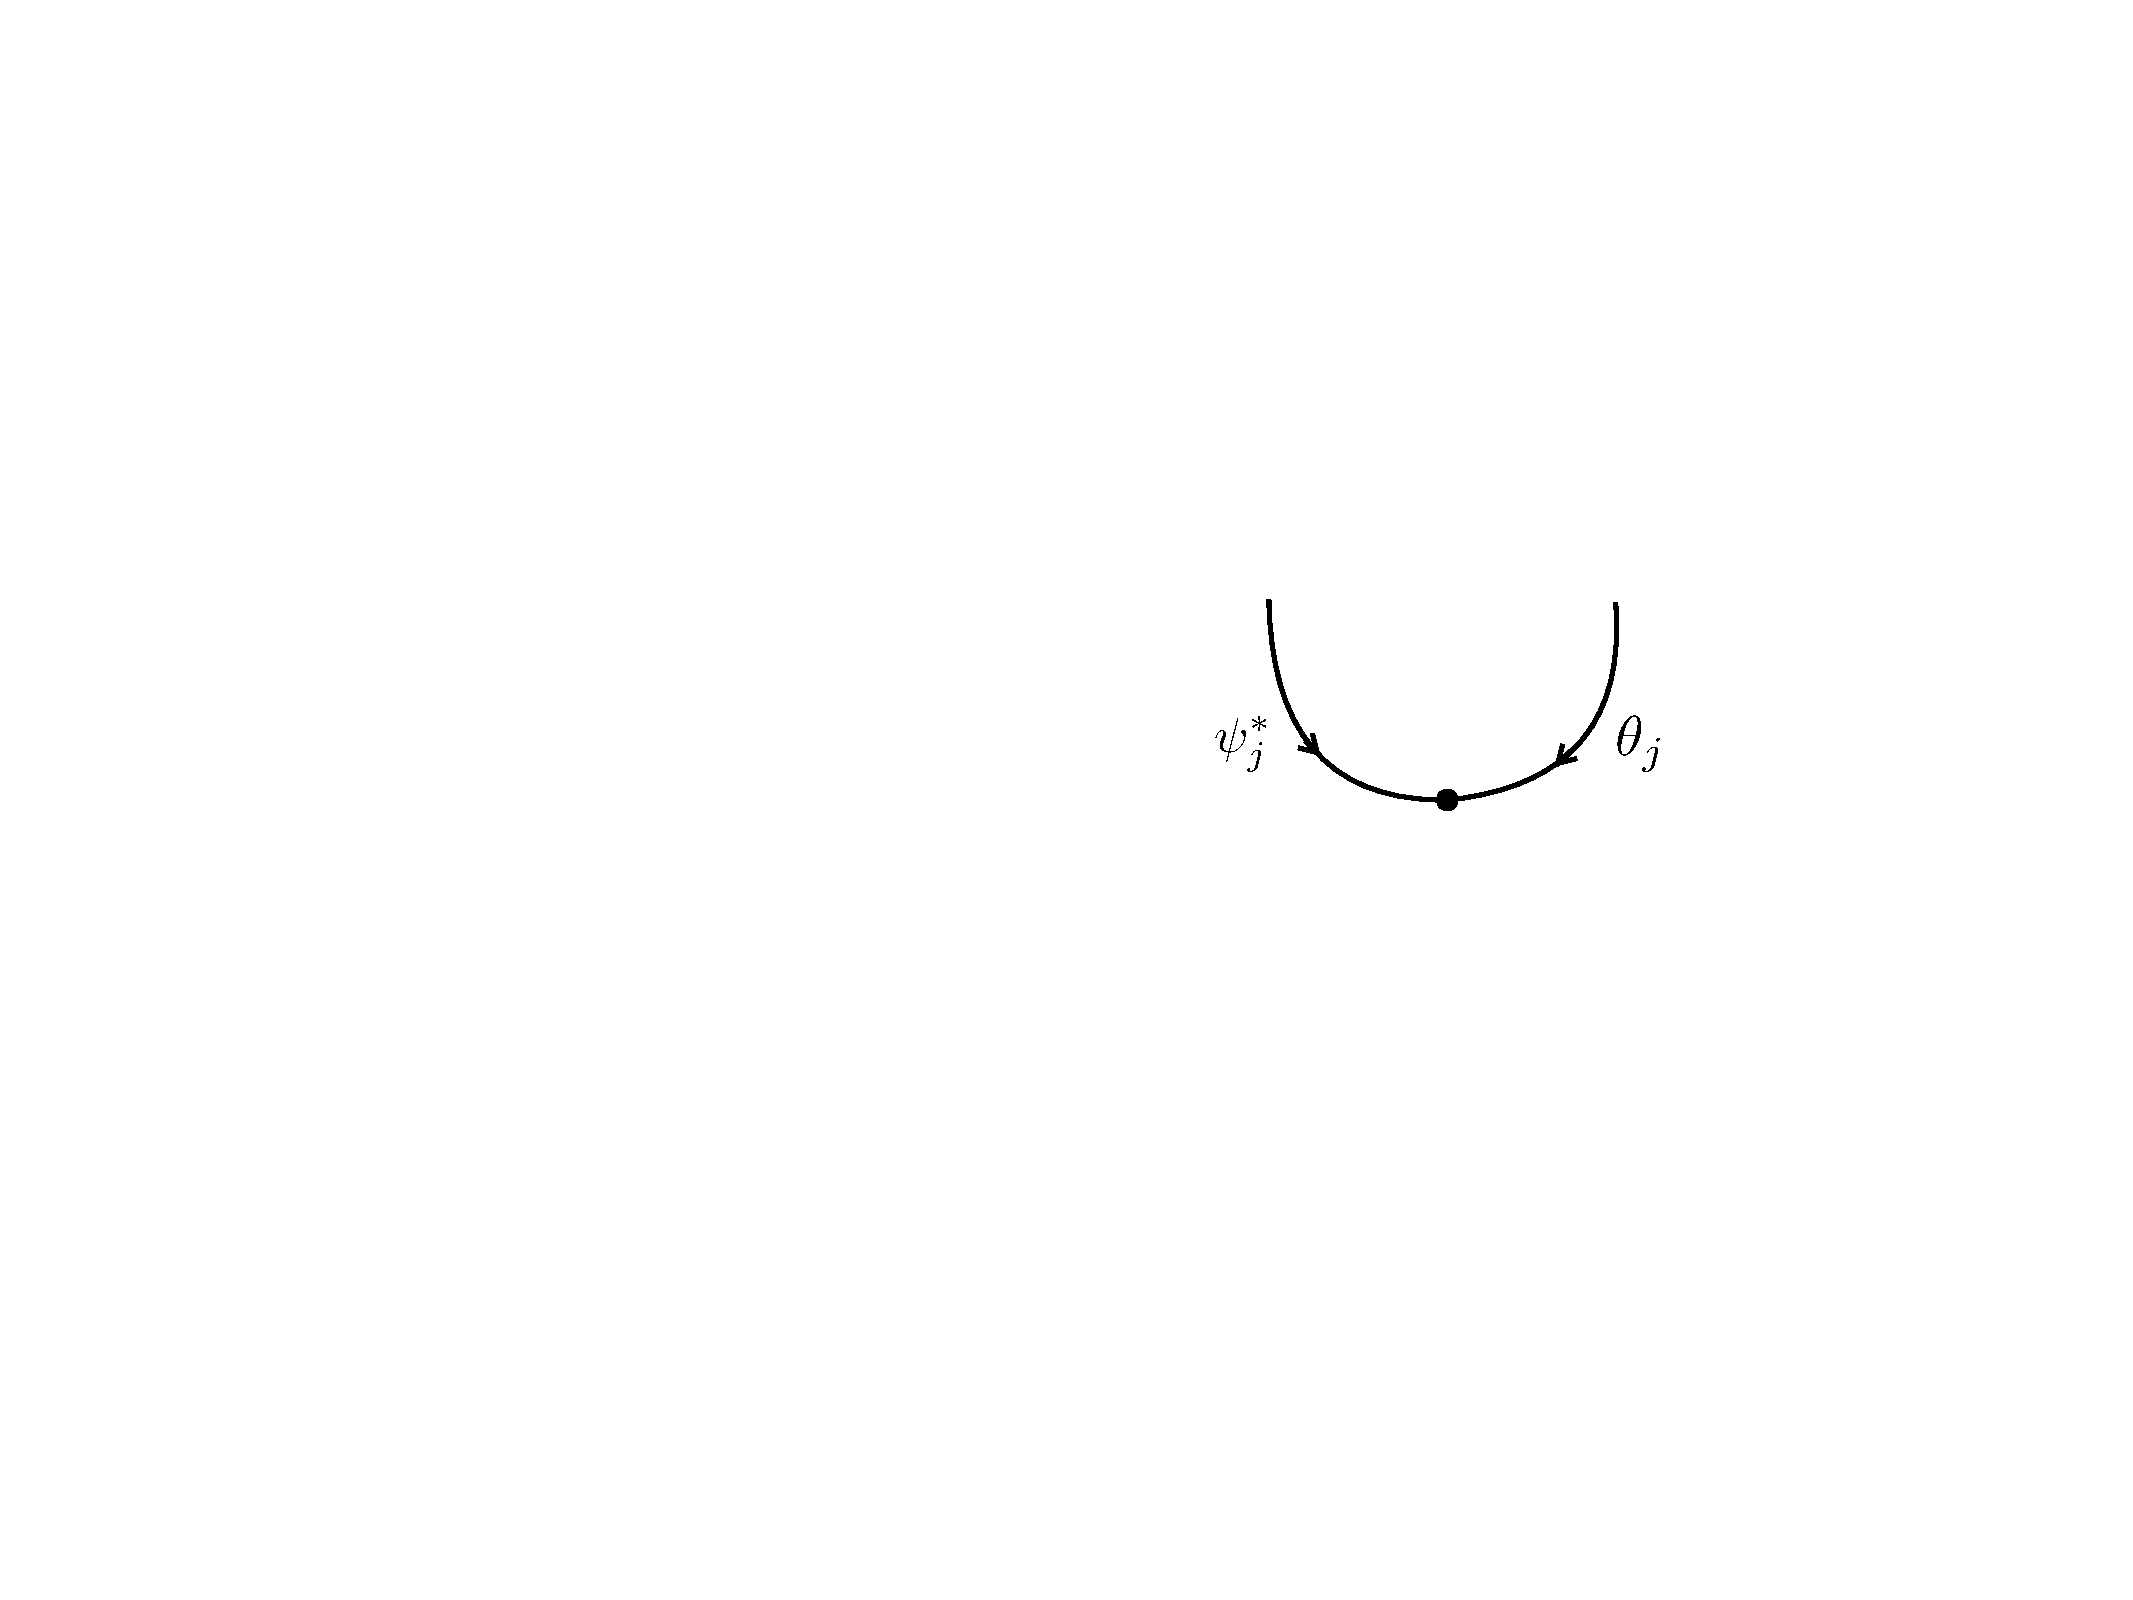
\includegraphics[scale=0.4]{dia4}
&
$m_2 \big( \big[\psi_j,-\big] \otimes \theta_j^* \big) \in \Hom_k( \HH^{\otimes 2}, \HH )$\\
\vspace{0.5cm}
$1 \le j \le n$
&
\tagarray{\label{interaction_3}}
\end{tabular}
\end{center}
Here $m_2$ is the multiplication in $\HH$ and, given $\gamma \in \mathbb{N}^n$, we write $x^\gamma = x_1^{\gamma_1} \cdots x_n^{\gamma_n}$, with $e_i \in \mathbb{N}^n$ the unit vector with $x^{e_i} = x_i$. By convention if $\gamma_a = 0$ then $x^{\gamma - e_a} = 0$, which ensures that we always have $\gamma_a x^{\gamma - e_a} = \partial_a(x^\gamma)$. Finally note that bosons are depicted with dotted lines, and fermions with solid lines.

These interactions ``take place'' at vertices of the tree $A(T)$ for some $T \in \cat{T}_q$, and come with the following constraints, which will be formalised below in terms of combinatorial data called \emph{configurations}. We write $f(\gamma)$ for the coefficient of $x^\gamma$ in a polynomial $f \in R$ and recall the chosen decomposition $W = \sum_j x_j W^j$. 

\begin{itemize}
\item A-type interactions only occur at input vertices and internal edges of $T$. 
\item B-type interactions only occur at internal edges of $T$.
\item C-type interactions only occur at internal vertices of $T$, and moreover the incoming lines must come from different branches of the tree.
\item There may be arbitrarily many A-type or C-type interactions per vertex of $A(T)$, but there is \emph{precisely one} B-type interaction at each internal edge of $T$.
\item The A-type interaction with indices $a,j, \gamma$ appears with the coefficient
\be\label{eq:coeff_a}
-\frac{\gamma_a}{|\gamma|} W^j( \gamma)\,.
\ee
where $|\gamma| = \sum_{i=1}^n \gamma_i$. Each B- and C-type interaction appears with coefficient $(-1)$.
\end{itemize}

As we will see, the coefficient \eqref{eq:coeff_a} is the only way that $W$ enters the rules, and thus the definition of the $A_\infty$-products on $\mathscr{B}$. The precise definition of the Feynman rules will be given in Definition \ref{defn:config} below, but first we give an example of a tree with interactions inserted, to illustrate the various ingredients.

\begin{example}\label{ex:picture_example} Consider the tree $T \in \cat{T}_3$ whose augmented tree $A(T)$ is depicted below, together with labels for its vertices, where we label by $e$ the vertex corresponding to the internal edge of $T$:
\begin{center}
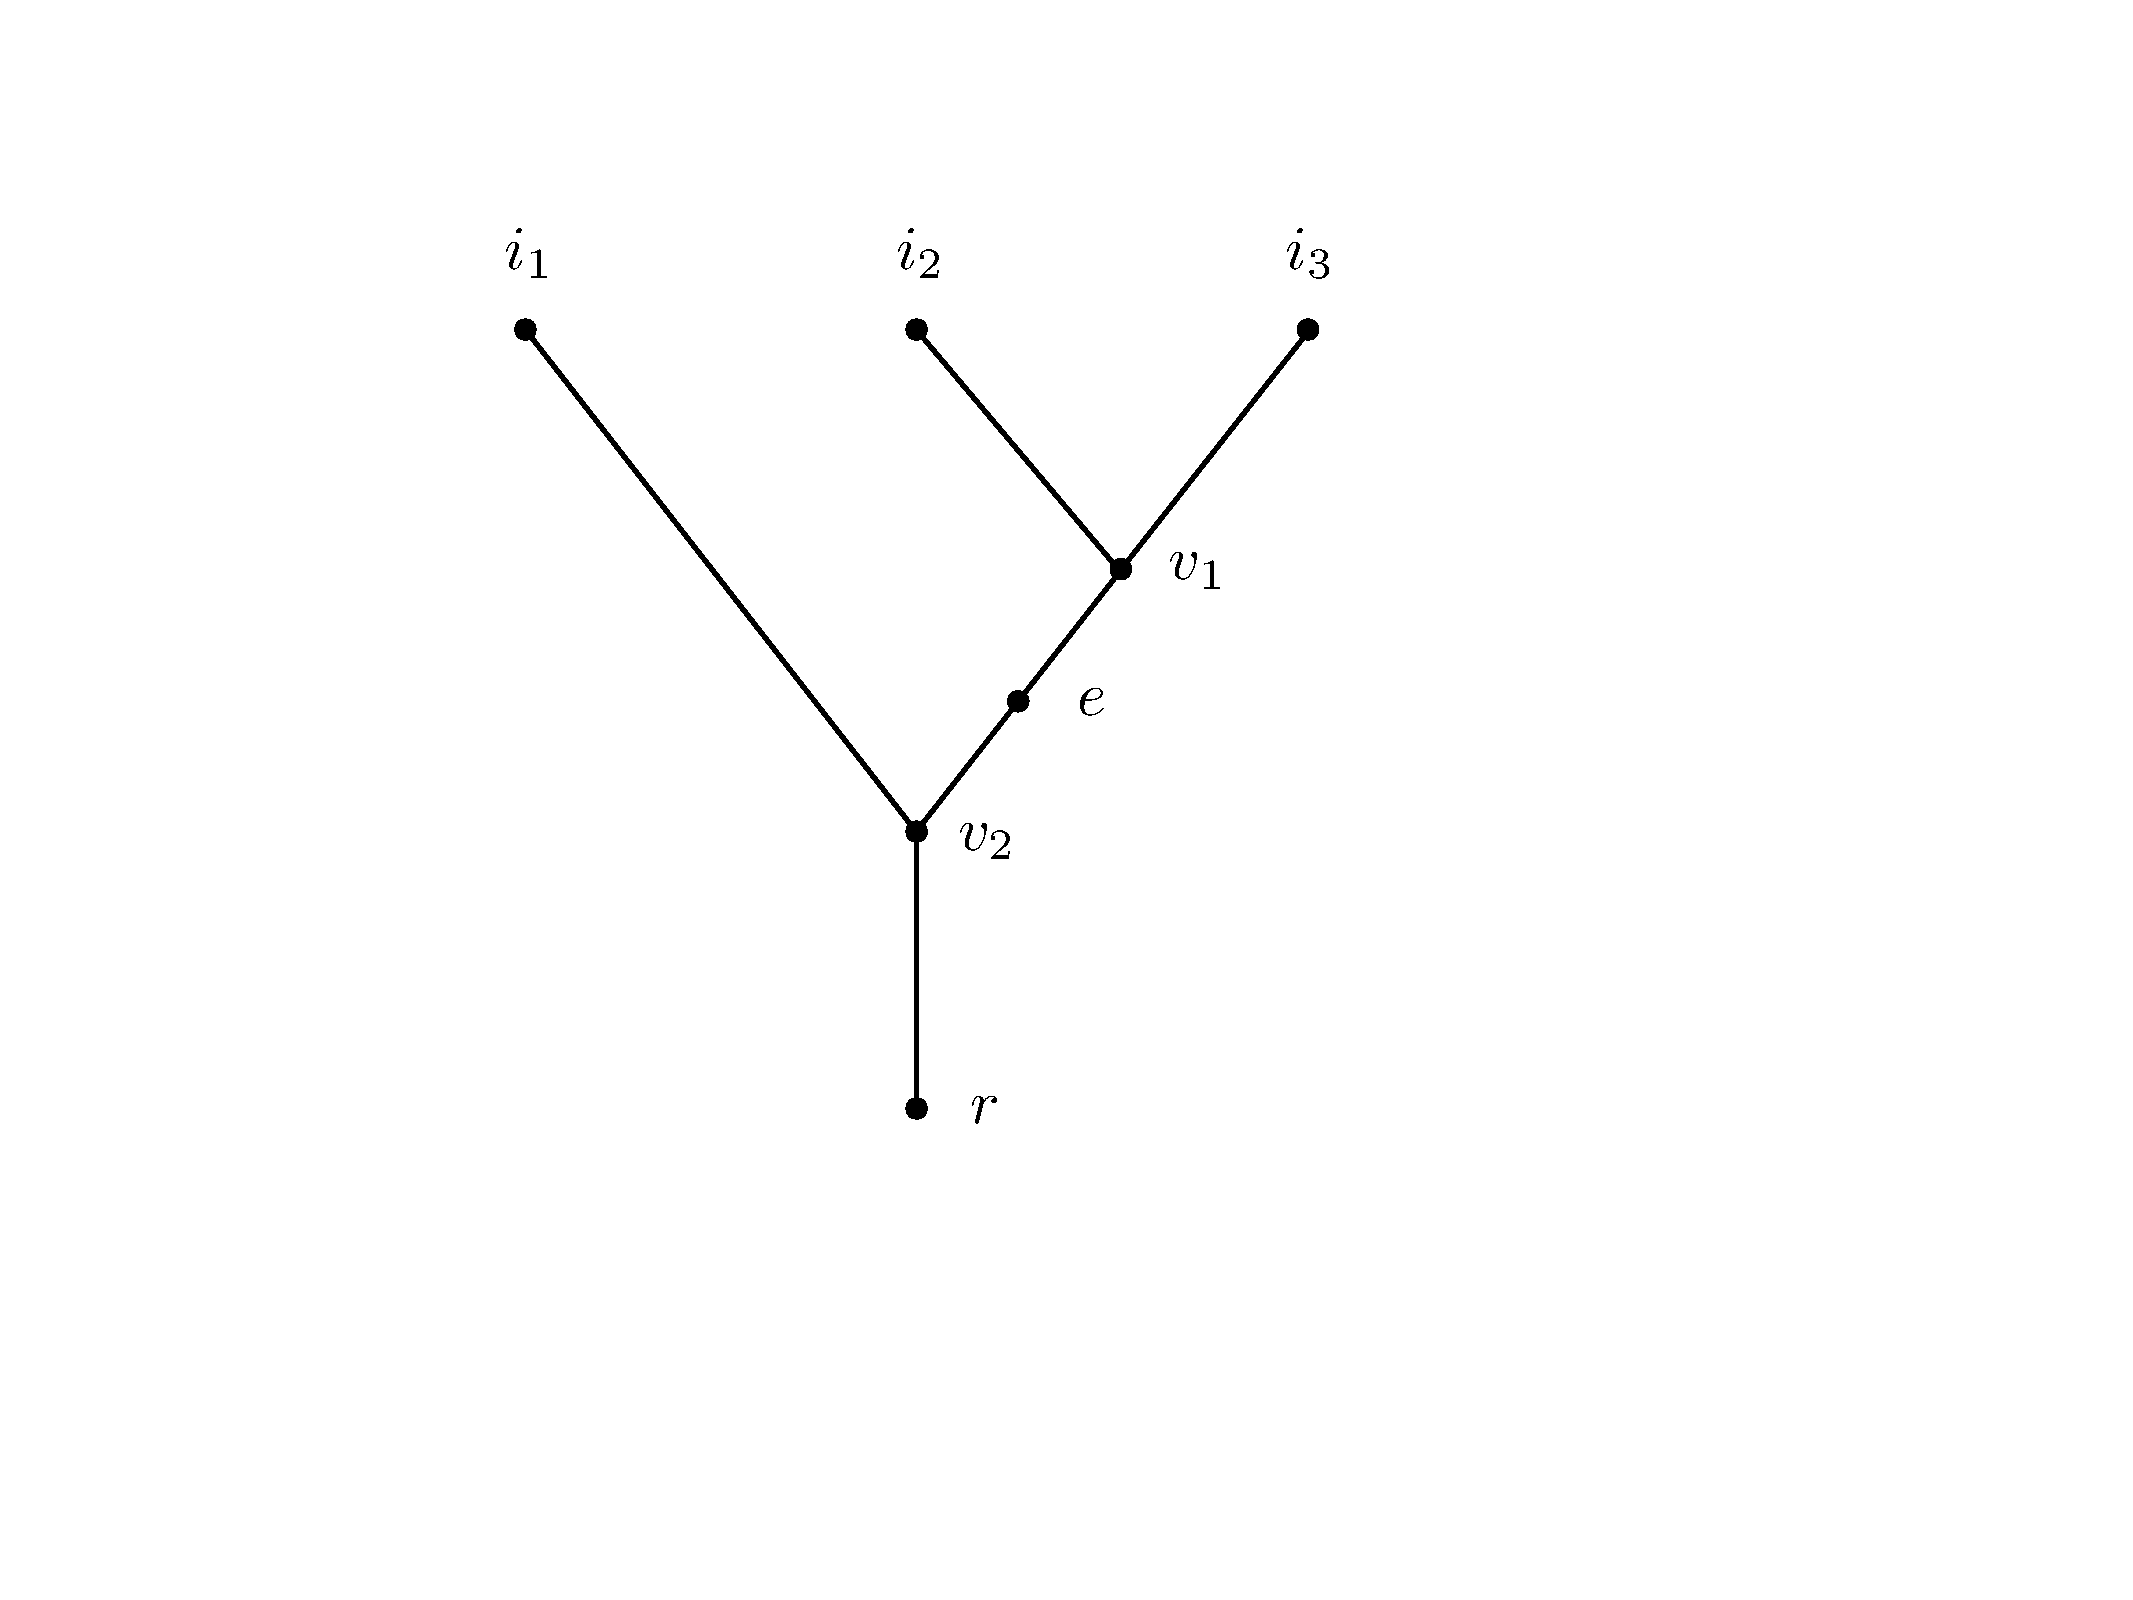
\includegraphics[scale=0.25]{dia7}
\end{center}
Set $W = x^3 \in \mathbb{C}[x]$ so that $W^1 = x^2$ and the only A-type interaction has $a = 1, j = 1, \gamma = 2$ and coefficient $-1$, as in the diagram (we write $\theta = \theta_1, \psi = \psi_1$)
\begin{center}
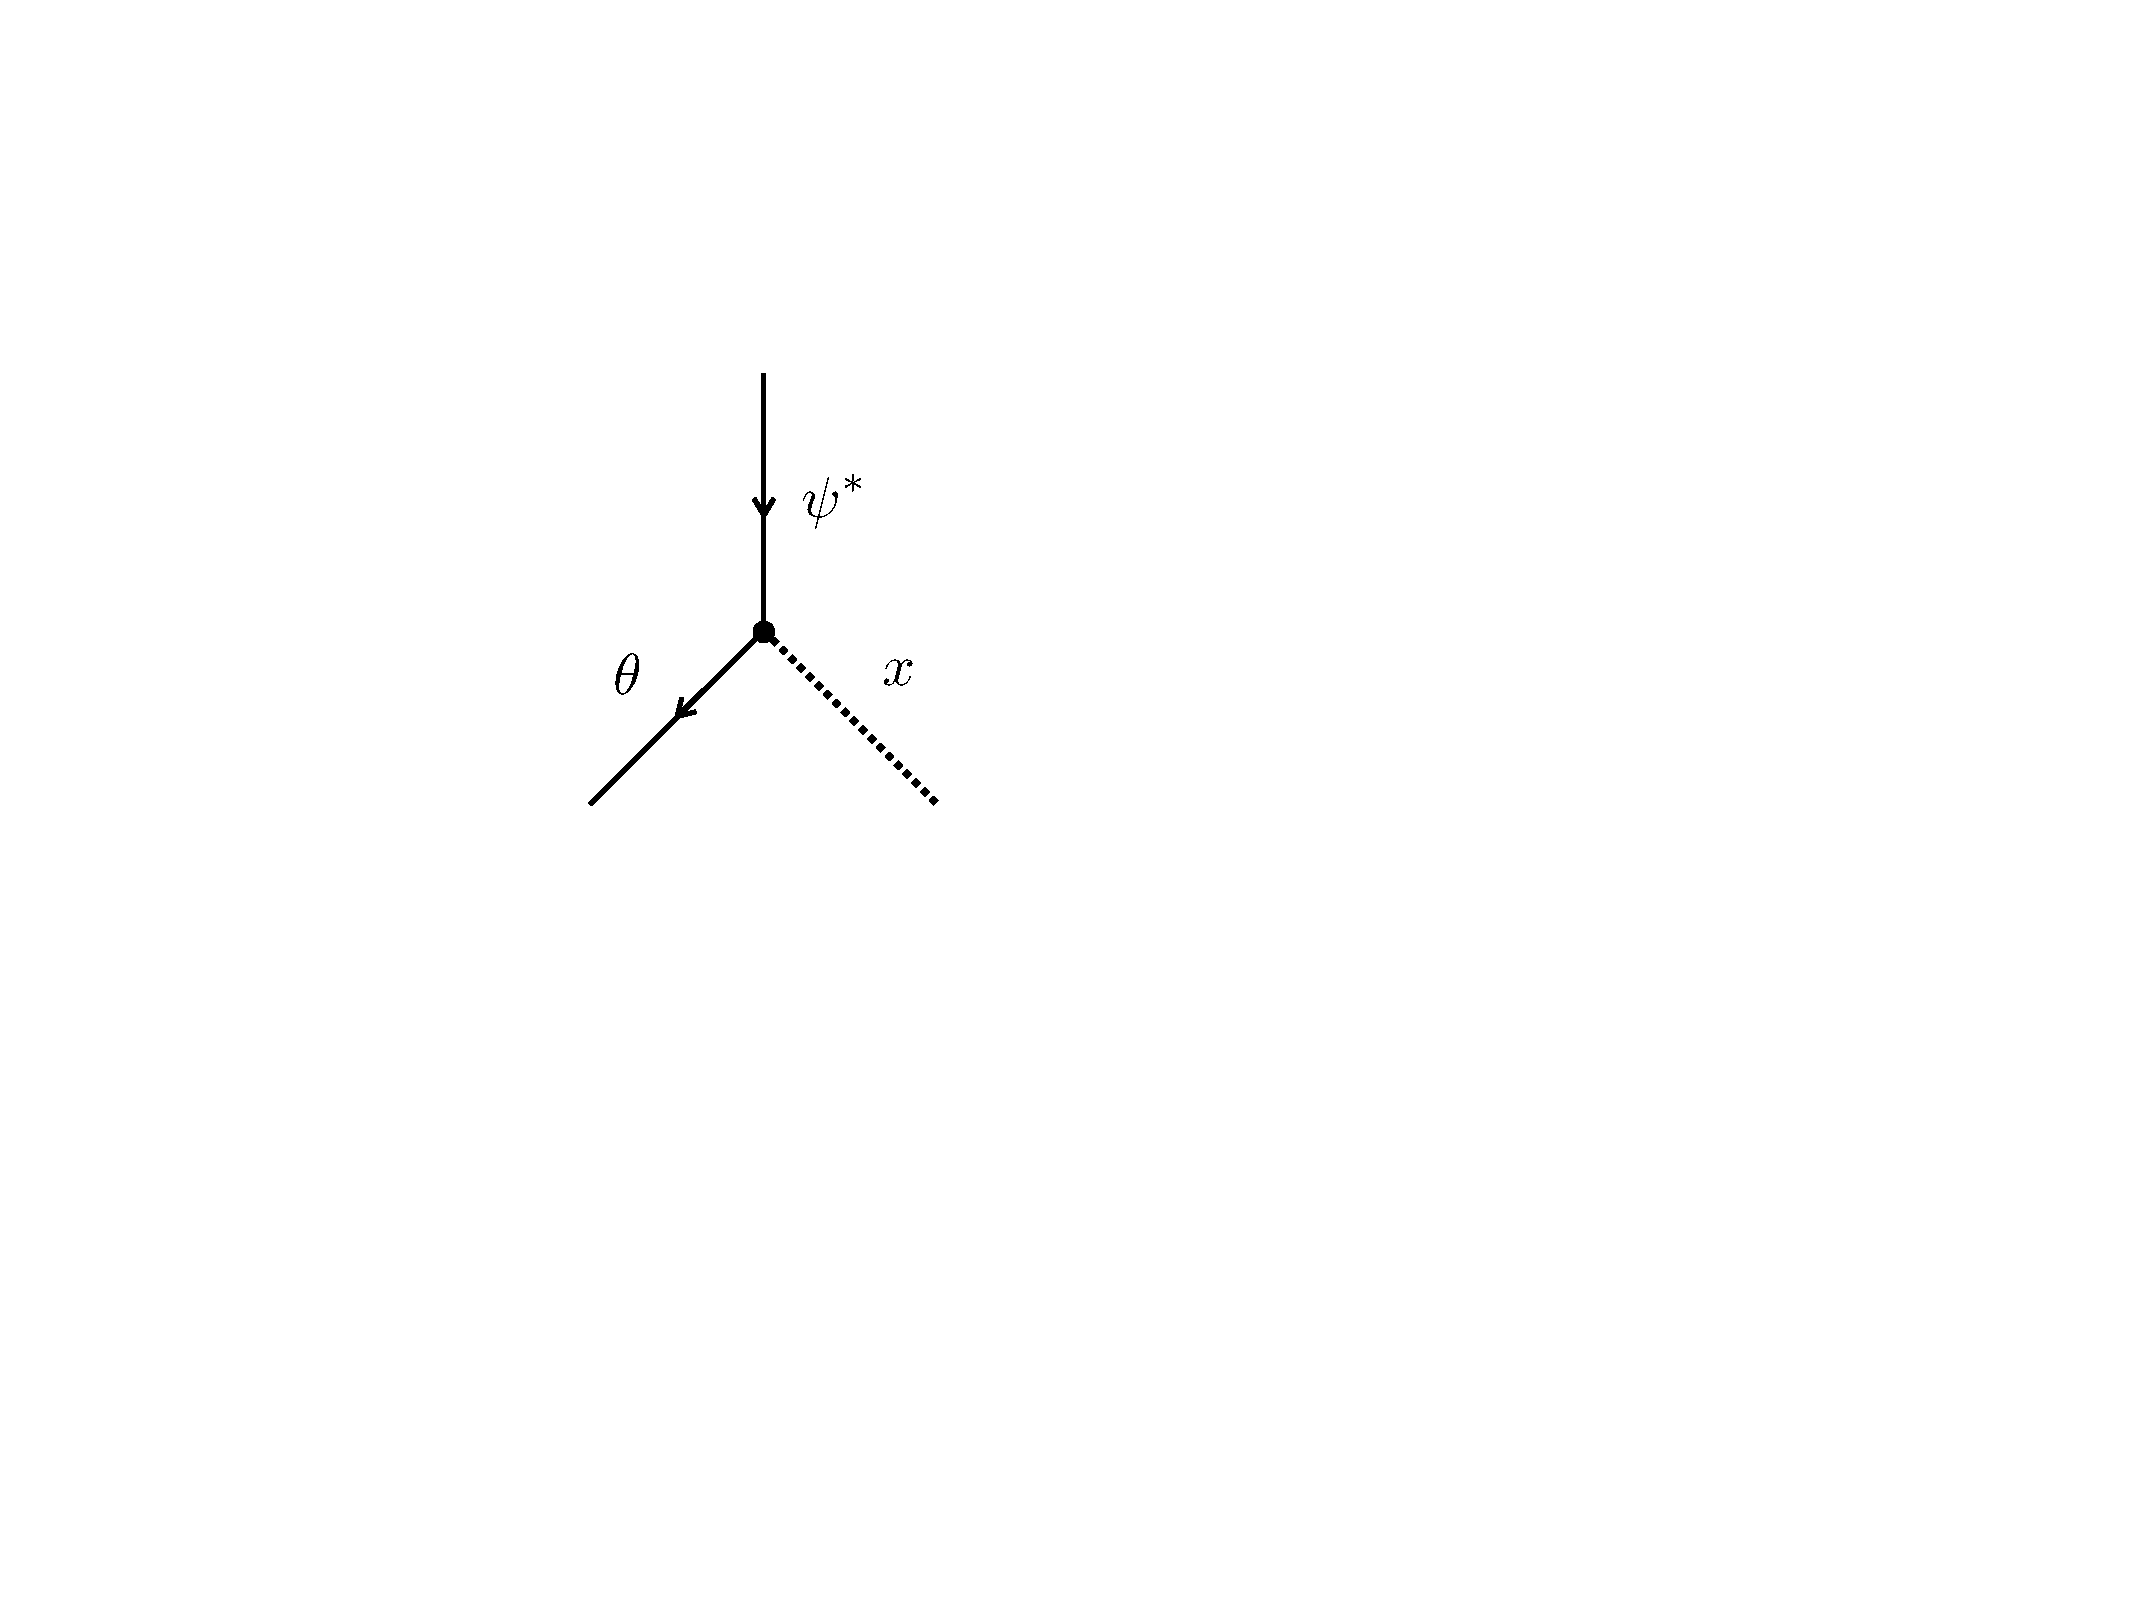
\includegraphics[scale=0.3]{dia5}
\end{center}
Consider the input state $\Psi = \psi^* \otimes \psi^* \otimes \psi^*$ in $\mathscr{B}^{\otimes 3}$. One possible pattern of interactions (called a configuration, below) has a single A-type interaction at the input vertex $i_3$, a B-type interaction at $e$, and two C-type interactions at $v_1,v_2$, as shown in the following ``topological'' Feynman diagram
\begin{center}
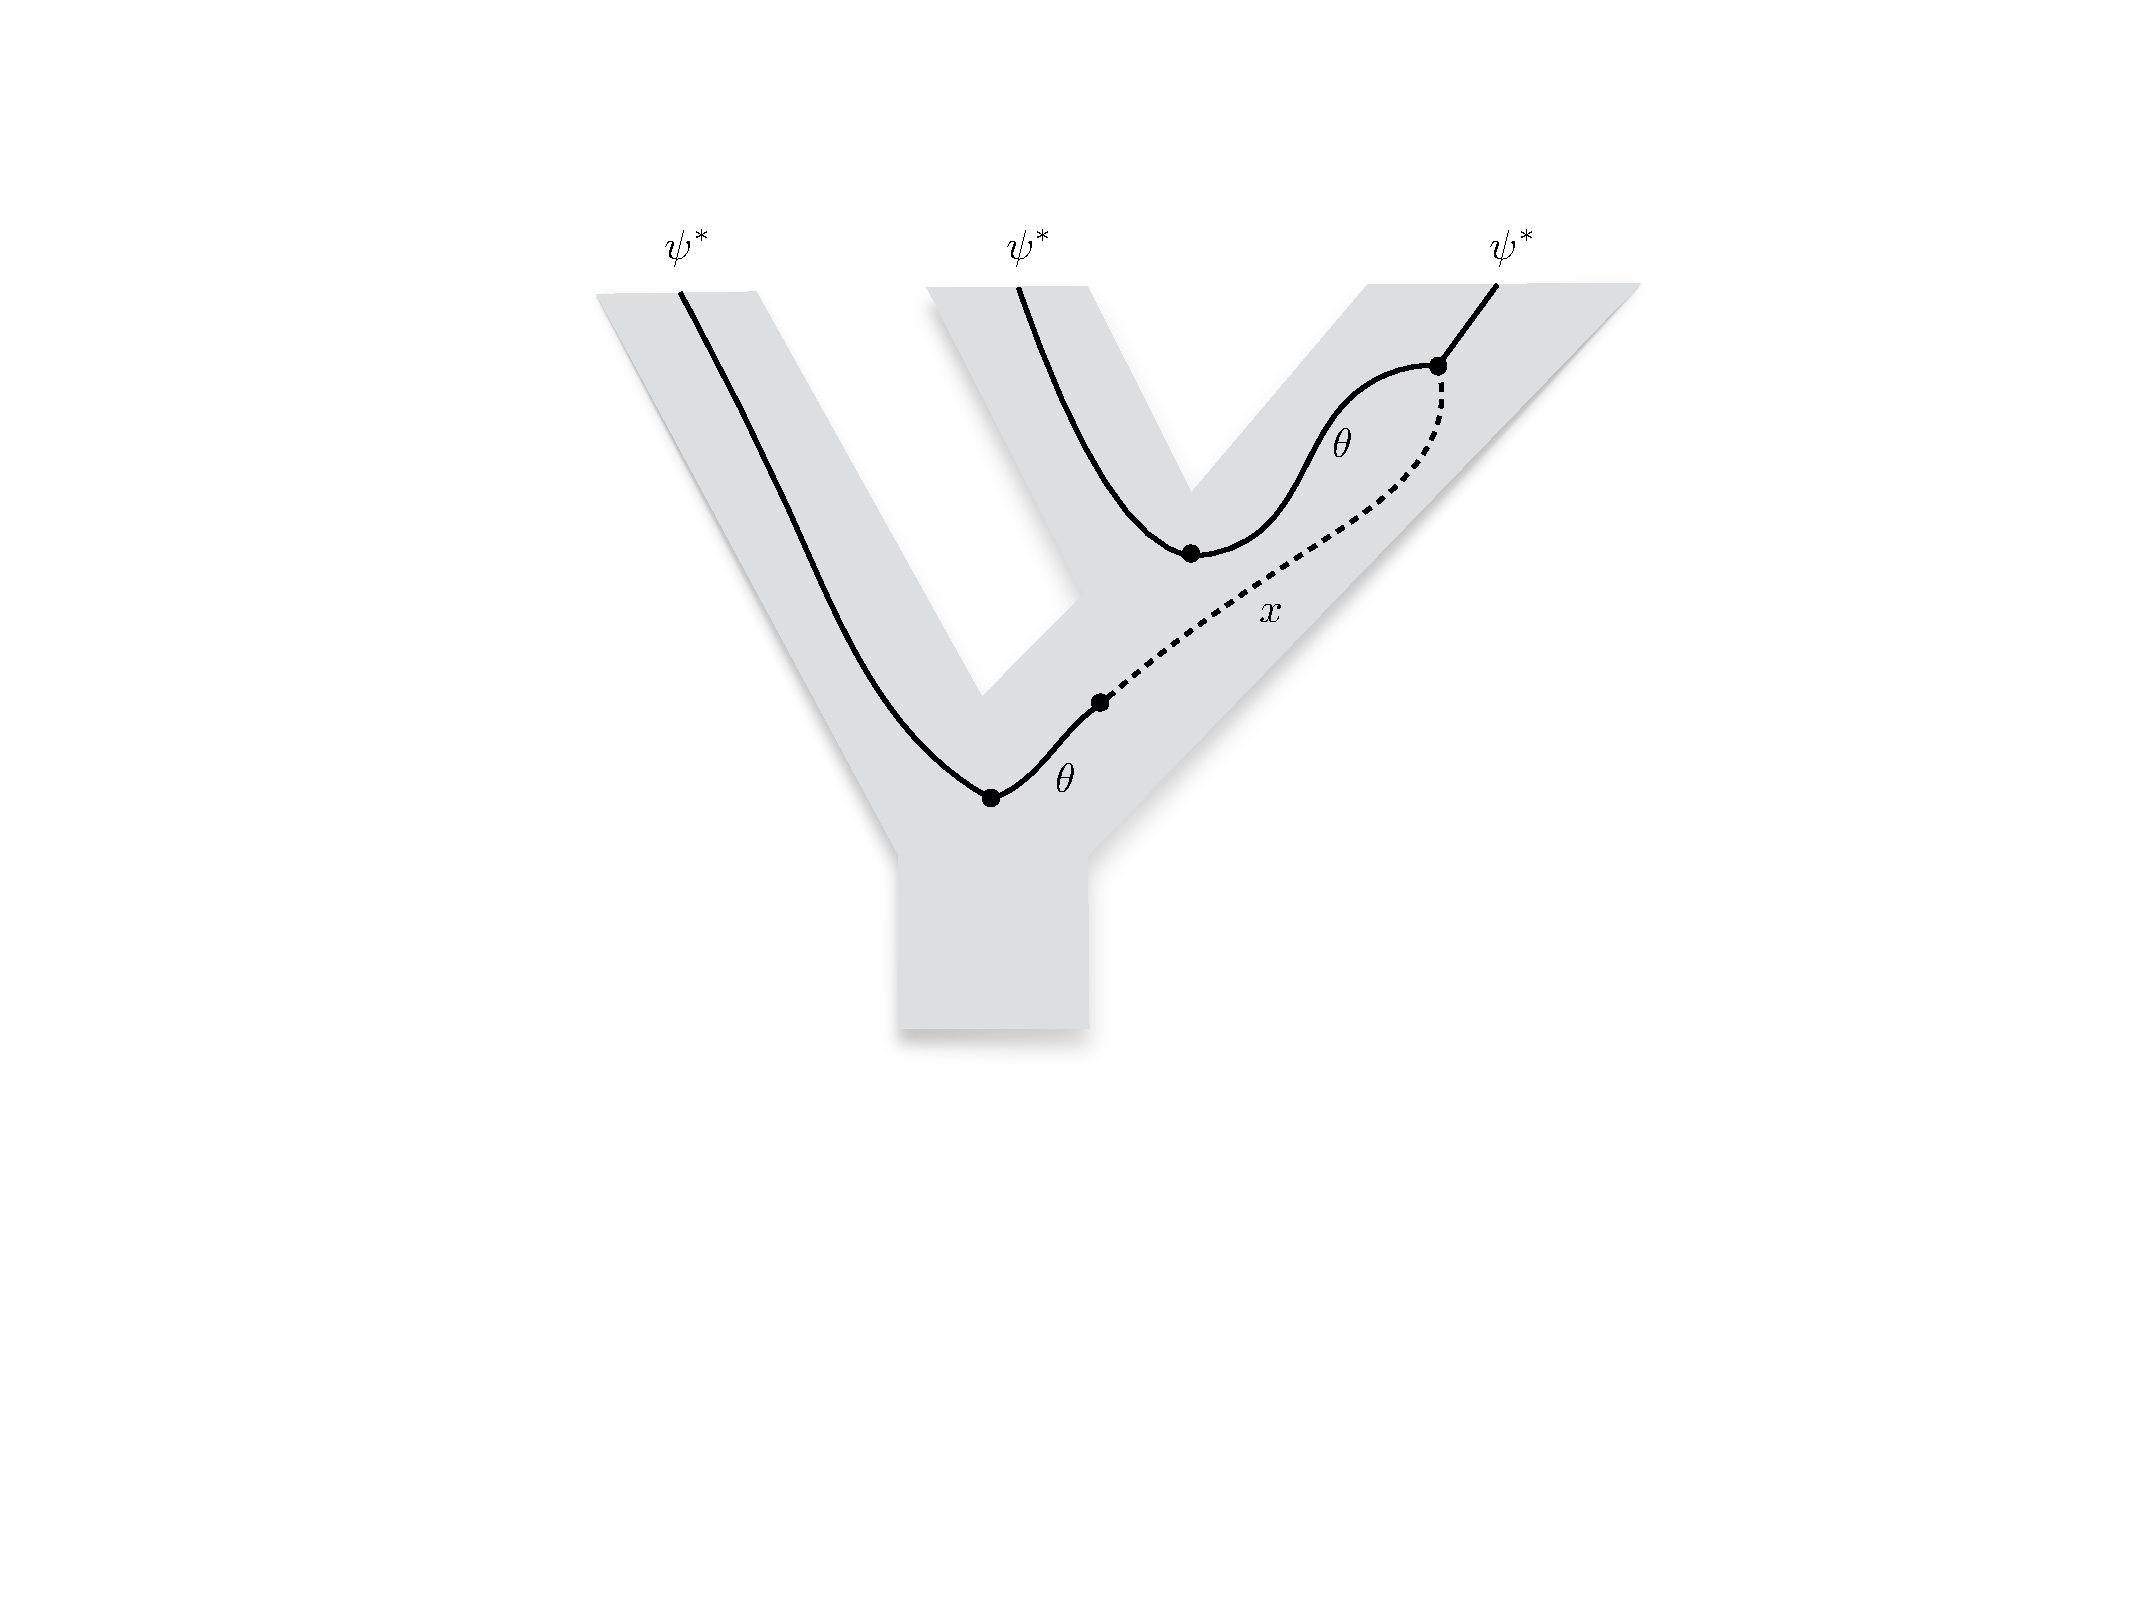
\includegraphics[scale=0.3]{dia6}
\end{center}
The \emph{value} of this diagram is the value of the linear map
\be\label{eq:operator_tree_example}
(-1)^3 p \circ m_2 \big([\psi, -] \otimes \theta^*\big) \circ \big( \sigma \otimes \theta \partial_x \circ m_2 ([\psi, -] \otimes \theta^*)\big( \sigma \otimes \theta x [\psi, -] \sigma \big)\big)
\ee
on the input state $\Psi$. Usually when evaluating such an expression we would pay attention to Koszul signs from commuting the input $\psi^*$'s into position (see Definition \ref{??}). Ignoring all signs, the value is
\begin{align*}
\pm \; & p \circ m_2 \big([\psi, -] \otimes \theta^*\big) \circ \big( \sigma \otimes \theta \partial_x \circ m_2 ([\psi, -] \otimes \theta^*)\big( \sigma \otimes \theta x [\psi, -] \sigma \big)\big)\Big( \Psi \Big)\\
&= \pm \; p \circ m_2 \big([\psi, \psi^*] \otimes \theta^* \theta \partial_x \circ m_2 ([\psi, \psi^*] \otimes \theta^* \theta x [\psi, \psi^*] \big)\big)\\
&= \pm \; p \circ m_2 \big(1 \otimes \theta^* \theta \partial_x \circ m_2 (1 \otimes \theta^* \theta x \big)\big)\\
&= \pm \; p \circ m_2 \big(1 \otimes \partial_x(x) \big)\\
&= \pm \; p(1) = \pm \; 1 \in \HH\,.
\end{align*}
\end{example}

Now we give some more precise definitions. Let $T \in \cat{T}_q$ be a valid plane tree with $q$ inputs and $e_i(T)$ internal edges, and let $A(T)$ be the augmented plane tree. The definitions are all relative to the ambient integer $n$, but for the sake of readability we will not reflect this in the notation.

We note that in the definition of the higher products $\rho_q$ below, any pair $(T,C)$ which has an internal edge $e$ with $N_C(e) = 0$ will not contribute to the sum in any case, so we do not care about $Z(T,C)$ for such configurations.

\begin{example} When $m(e) = 1, J(e) = \{ j \}$ and we write $\gamma = \gamma_j(e), N = \traff_C(e)$, we have
\[
\samp_{\traff_C(e)}\big( \underline{\gamma}(e) \big) = \frac{|\gamma|}{N + |\gamma|}\,.
\]
In the case where $m(e) = 2, J(e) = \{ j, j' \}$ and we write $\gamma = \gamma_j(e), \gamma' = \gamma_{j'}(e)$,
\[
\samp_{\traff_C(e)}\big( \underline{\gamma}(e) \big) = \frac{|\gamma||\gamma'|}{N + |\gamma| + |\gamma'|} \left( \frac{1}{N + |\gamma|}  + \frac{1}{N + |\gamma'|}\right)\,.
\]
In particular, for the tree and configuration of Examples \ref{ex:picture_example}, \ref{ex:picture_example_2} we only have one internal edge $e$ with $m(e) = 0$, so $Z(T,C) = \frac{1}{N_C(e)} = 1$.
\end{example}

\begin{example} The potential $W = x^d$ for $d > 2$ has the following Feynman rules:
\begin{center}
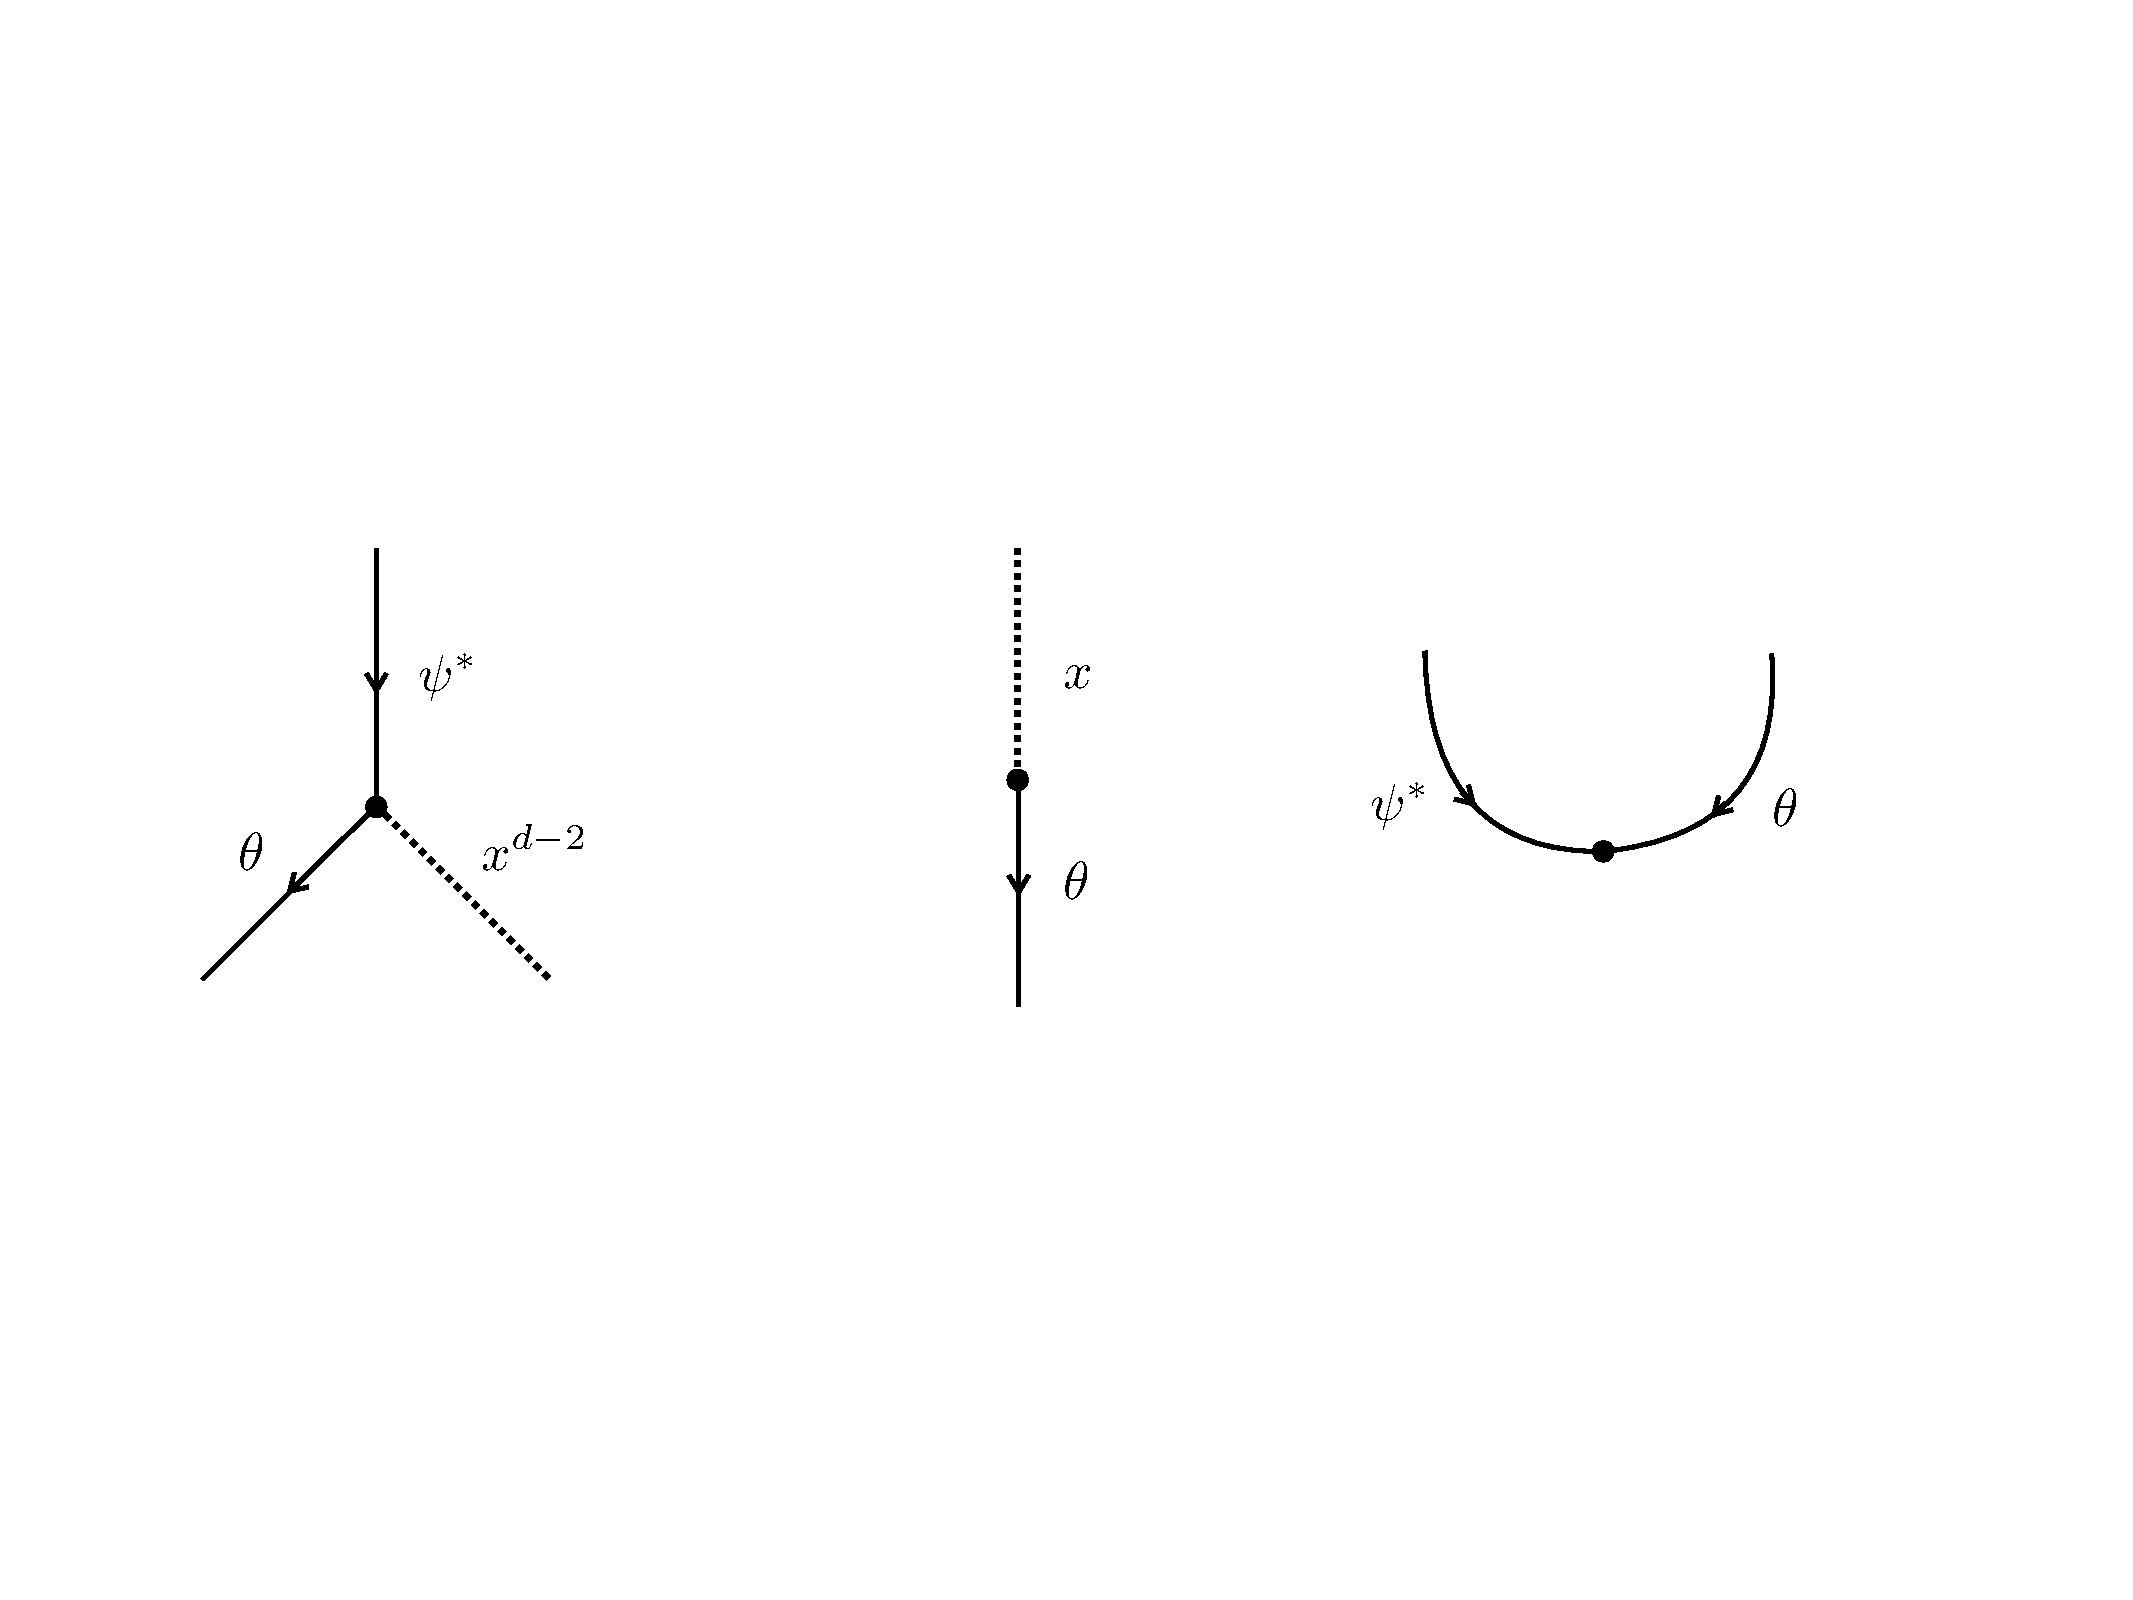
\includegraphics[scale=0.45]{dia9}
\end{center}
Let us compute the $A_\infty$-products $\rho_q$ on $\mathscr{B}$:
\begin{itemize}
\item For $q = 2$ there is only one tree $T \in \cat{T}_2$. We claim that since $T$ has no internal edge the only configuration $C$ with $\cat{O}(T,C) \neq 0$ is the unique $C$ with no A-type or C-type interactions (see Remark \ref{remark:config_count}). To see this, note that an A-type interaction would create a polynomial $x^{d-2}$ which cannot be eliminated by derivatives at internal edges, and therefore annihilates with $p$. Since there can be no A-type interaction to create a $\theta$, the $\theta^*$ in a C-type interaction will end up acting on the identity in the exterior algebra, and giving zero as well. Since this $C$ is the only contributor to the sum, and $\langle D_{T,C} \rangle = p \circ m_2 \circ (\sigma \otimes \sigma)$, we have
\be\label{eq:a_type_product}
\rho_2( \Lambda_2, \Lambda_1 ) = (-1)^{\widetilde{\Lambda_1} \widetilde{\Lambda_2} + \widetilde{\Lambda_1} + 1} \Lambda_1 \cdot \Lambda_2
\ee
where $(-) \cdot (-)$ denotes the usual product in the exterior algebra. This is just the forward suspension of the product in the exterior algebra.

\item For $q > 2$ let $C$ be a configuration with $\cat{O}(T,C) \neq 0$. Then $C$ must have at least one A-type interaction, since otherwise the $\partial_x$ in the B-type interactions are applied to $1 \in R$. Moreover, these A-type interactions can only be inserted at input vertices, since at an internal edge \eqref{eq:int_intedge} would contribute $\theta^2 = 0$.

For the same reason, the $\theta$ coming out of the B-type interaction at an internal edge $e$ must be consumed in a C-type interaction at the vertex $v$ immediately after $e$ on the path to the root: if not, it will annihilate with the $\theta$ emitted at the next internal edge, or, if $v$ is adjacent to the root, it will annihilate with $p$. This means that every edge $e$ must be the right-hand branch at $v$, from which we deduce that $T$ is the tree in which all internal edges lie on the path from the rightmost input to the root:
\begin{center}
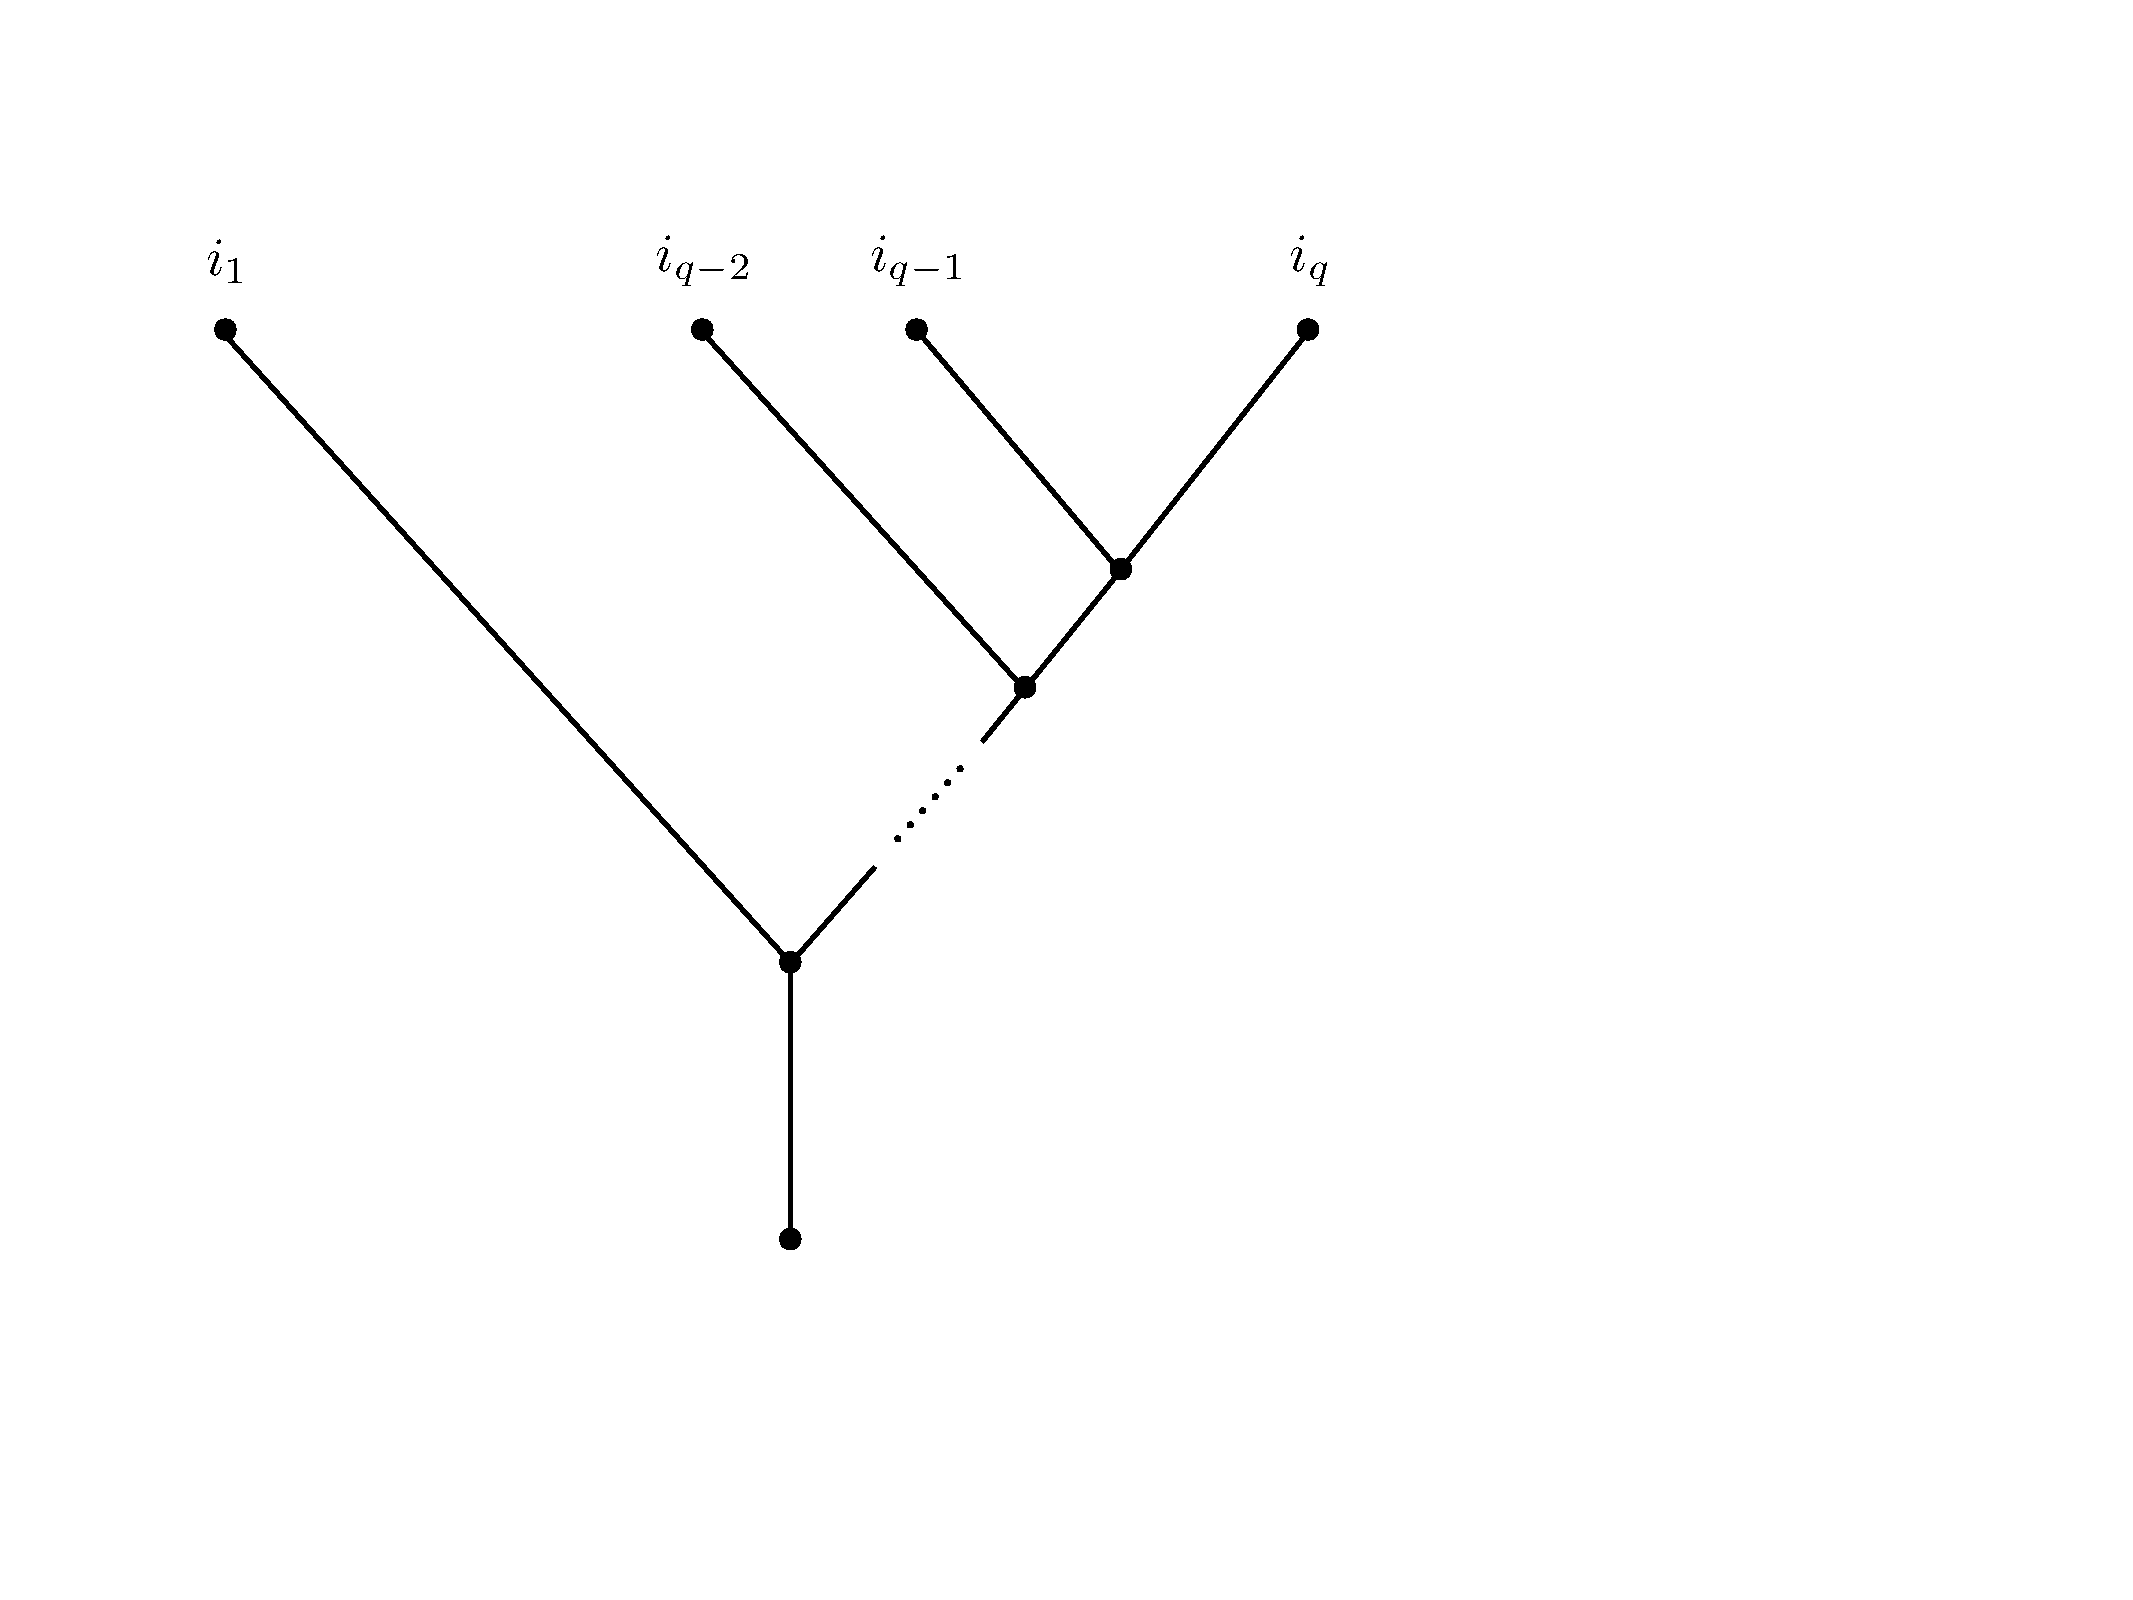
\includegraphics[scale=0.3]{dia10}
\end{center}
This implies that there is \emph{precisely} one A-type interaction in $C$, and it takes place at the vertex marked $i_q$ in the diagram. But since $T$ contains $q - 2$ internal edges, if $\cat{O}(T,C) \neq 0$ then we must have $q = d$. That is, $\rho_q = 0$ unless $q \in \{2,d\}$.

\item Finally, let us describe $\rho_d: \mathscr{B}^{\otimes d} \lto \mathscr{B}$ on the basis of tensors $(\psi^*)^{s_0} \otimes \cdots \otimes (\psi^*)^{s_d}$ where $s_j \in \{0,1\}$ for $1 \le j \le d$. We require a copy of $\psi^*$ at each input $i_1,\ldots,i_{q-2}$ in order to meet the $\theta$ emitted by B-type interactions, a copy of $\psi^*$ at $i_{q-1}$ to meet the $\theta$ from the A-type interaction and a $\psi^*$ at $i_q$ to initiate that A-type interaction. Hence $\rho_d$ is zero on all the basis elements except for
\[
\rho_d( \psi^* \otimes \psi^* \otimes \cdots \otimes \psi^* ) = (-1)^{Q(T, \underline{\Lambda})} \cdot 1\,.
\]
To compute the sign, observe that $e_i(T) = d - 2$ and $\Lambda_i = \psi^*$ is odd so $\widetilde{\Lambda_i}$ is even, whence $Q(T, \underline{\Lambda}) = (d-2) + d + 1 = 1$.
\end{itemize}
In summary: the underlying $\nZ_2$-graded $k$-module of $\mathscr{B}$ is the exterior algebra $\bigwedge( k \psi^* )$ and the $A_\infty$-products $\rho_q$ are zero unless $q \in \{ 2, d \}$. The product $\rho_2$ is the forward suspended version of the usual product on the exterior algebra, while
\[
\rho_d( \psi^* \otimes \psi^* \otimes \cdots \otimes \psi^* ) = -1\,.
\]
\end{example}

\subsection{Atiyah classes and idempotents}
% ainfmf12

The endomorphism algebra $C = \End_k(S)$ is a Clifford algebra generated by the contraction $\theta_i^*$ and wedge product $\theta_i$ operators. It is observed in \cite{murfet} that \eqref{eq:he_start} is an isomorphism of Clifford representations (in the homotopy category) when the complex $\md{E}$ is equipped with the action induced by Atiyah classes:

\begin{definition}
The Atiyah classes of $\md{A}_W$ are the $R$-linear odd operators
\[
\At_i = [\partial, \partial_{i}]: \End_R(k^{\stab}) \lto \End_R(k^{\stab})\,,
\]
\end{definition}

\begin{lemma} We have
\[
\At_i = -[\psi_i^*, -] - \sum_{q=1}^n \partial_{i}(W^q) [ \psi_q, - ]\,.
\]
\end{lemma}
\begin{proof}
By direct calculation:
\begin{align*}
\At_i &= \big[ [d_{k^{\stab}},-], \partial_{i} \big]\\
&= \sum_q \big[x_q [\psi_q^*,-], \partial_{i}\big] + \sum_q \big[W^q [\psi_q,-], \partial_{i}\big]\\
&= -\sum_q \partial_{i}(x_q) [\psi_q^*,-] - \sum_q \partial_{i}(W^q) [\psi_q,-]\\
&= -[\psi_i^*,-] - \sum_q \partial_{i}(W^q) [\psi_q, -]\,.
\end{align*}
\end{proof}

\begin{lemma} The induced Clifford algebra structure on $\mathscr{E}$ is given by
\[
\gamma_i^\dagger = \At_i = -[\psi_i^*, -]\,, \qquad \gamma_i = -\psi_i\,.
\]
\end{lemma}

\begin{lemma} The idempotent $e = \gamma_1^\dagger \cdots \gamma_n^\dagger \gamma_n \cdots \gamma_1$ is the projection onto $\mathscr{B} \subseteq \mathscr{E}$.
\end{lemma}

\textbf{Feynman diagrams.} The construction of the higher operations $m_n$ and the idempotent $\widetilde{e}$ is given in terms of Feynman diagrams, as we will now briefly explain. The functions $m_n$ are $k$-linear maps parametrised by sequences of matrix factorisations $X_0,\ldots,X_n$
\[
m_n: \bigotimes_{i=0}^{n-1}\big[ R/I \otimes_R \md{C}(X_i,X_{i+1}) \big] \lto R/I \otimes_R \md{C}(X_0,X_n)
\]
The minimal model construction gives a formula for this operation as a sum over trees of contractions of operators derived from the differential on $\md{C}$ and the connection $\nabla$ mentioned above. These contractions are similar to those of creation and annihilation operators in the calculation of S-matrix elements in quantum field theory \cite{??}. A powerful method for organising such calculations was discovered by Feynman, and his diagrams may be used to present the higher operations $m_n$ in terms of a short list of \emph{interaction vertices}. To present these vertices, let $(X,Y)$ be a consecutive pair of matrix factorisations $(X_i, X_{i+1})$ in our list and choose homogeneous $R$-bases for these matrix factorisations so as to write
\be\label{eq:choose_basis}
\md{C}( X, Y ) \cong \Hom_k( \widetilde{X}, \widetilde{Y} ) \otimes R
\ee
for some $\nZ_2$-graded $k$-vector spaces $\widetilde{X},\widetilde{Y}$. Each interaction vertex in a Feynman diagram is a graphical representation of an operator on a vector space of the form
\be\label{eq:virtual_space}
\bigwedge F_\theta \otimes R/I \otimes \Hom_k( \widetilde{X}, \widetilde{Y} )  \otimes \, k\llbracket t_1,\ldots,t_n \rrbracket
\ee
where the sequence of partial derivatives of the potential $(t_1,\ldots,t_n) = (\partial_{x_1} W,\ldots,\partial_{x_n} W)$ is a quasi-regular sequence which acts null-homotopically on $\md{C}(Y,Y)$ and we choose null-homotopies $\lambda_j: Y \lto Y$ so that $[d_{Y}, \lambda_j] = t_j \cdot 1_{Y}$. As we will recall in Section \ref{??} there is a $k\llbracket \bold{t} \rrbracket = k\llbracket t_1,\ldots,t_n \rrbracket$-linear isomorphism
\[
\sigmastar: R/I \otimes k \llbracket \bold{t} \rrbracket \lto \widehat{R}\,.
\]
An element $r \in R$ acts by multiplication on the right hand side, and so by a $k\llbracket \bold{t} \rrbracket$-linear operator on the left hand side. In this way the differential $D$ of $\md{C}(X,Y)$, viewed as a matrix with respect to the chosen $R$-basis \eqref{eq:choose_basis}, may be viewed as acting on the vector space \eqref{eq:virtual_space}. With this notation the interaction vertices are
\begin{itemize}
\item (A-type) $[ D, \nabla ]$ the critical Atiyah class.
\item (B-type) $\nabla = \sum_i \partial_{t_i} \theta_i$
\item (C-type) $\sum_i \lambda_i^\bullet\, \theta_i^*$ where $\lambda^\bullet_i$ is the operator of post-composition with $\lambda_i$.
\end{itemize}
The analogy to Feynman diagrams is complete in the case when both $X,Y$ are of Koszul type \cite{??} so that the underlying graded modules $\widetilde{X}, \widetilde{Y}$ are exterior algebras and the operator $D$ on $\md{C}(X,Y)$ is a polynomial in creation and annihilation operators.
\\

We view $\Psi_1 \otimes \cdots \otimes \Psi_q \in \mathscr{B}^{\otimes q}$ as the result of applying creation operators (meaning wedge products $\psi_i^* \wedge -$) to the vacuum (meaning the identity of the exterior algebra) in the various copies of $\mathscr{B}$. The value of $\cat{O}(T,C)$ on $\Psi$ may be computed by commuting all creation operators acting on $\mathscr{H}$ (that is, the operators $x_i, \theta_i, \psi_i^*$) leftward in the expression, which means \emph{down} the tree. These operators commute with all other creation operators and with those annihilation operators that are either of a different type (e.g. $[x_i, \theta_j^*] = 0$) or of same type but with different indices (e.g. $[x_1, \partial_2] = 0$). However, there will be a nonzero commutator every time a creation operator meets an annihilation operator of the same type and index (respectively $\partial_i, \theta_i^*, [\psi_i, -]$). We view such a commutator, say
\[
\theta_i \theta_i^* + \theta_i^* \theta_i = [ \theta_i, \theta_i^* ] = 1\,,
\]
which arises as the result of commuting the $\theta_i$ leftward to meet the $\theta_i^*$, as generating two diagrams, corresponding to the two choices of summands in $\theta_i^* \theta_i = 1 - \theta_i \theta_i^*$. Choosing the first summand means there is an interaction (drawn as a line marked $\theta_i$ from the original position of the $\theta_i$ to the position of the $\theta_i^*$ in the tree) while choosing the second summand means there is no interaction (the $\theta_i$ sails on, to meet its partner further down the tree). If a particular series of choices leads to an $x_i$ or $\theta_i$ meeting the bottom of the tree then this diagram does not contribute to $\cat{O}(T,C)(\Psi)$ since $p$ projects out such elements of $\mathscr{H}$. 

Note that in this example one of the other series of ``choices'' would involve commuting the rightmost $\theta$ past the first $\theta^*$ to meet with the leftmost $\theta^*$. In the corresponding Feynman diagram the $\theta$ fermion would travel from the A-type interaction vertex all the way to the bottom of the tree. However, this diagram gives a zero contribution to $\cat{O}(T,C)(\Psi)$, for at least two reasons: firstly, in the calculation we see parallel identical fermion lines which vanish (since $\theta^2 = 0$), and secondly the leftmost $\theta$ may in this case be commuted left to give zero on $p$, after the ``guard'' $\theta^*$ is cancelled by the other $\theta$.

\begin{definition}\label{defn:config} A \emph{configuration} $C$ of a valid plane tree $T$ consists of the following data, for each non-root vertex $v$ of $A(T)$:
\begin{itemize}
\item An integer $m(v) \ge 0$.
\item A subset $J(v) \subseteq \{ 1,\ldots, n \}$ with $|J(v)| = m(v)$. 
\item If $v$ is an input, or comes from an internal edge of $T$, a pair
\[
( a_j(v), \gamma_j(v) ) \in \{ 1, \ldots, n \} \times \mathbb{N}^n
\]
for each $j \in J(v)$, with $\gamma_j(v)_{a_j(v)} \ge 1$.
\item If $v$ comes from an internal edge of $T$, an integer $t(v) \in \{1,\ldots,n\}$.
\end{itemize}
Let $\operatorname{Con}(T)$ denote the set of all configurations.
\end{definition} 

\begin{remark}\label{remark:config_count} The integer $m(v)$ counts how many interactions of type A or C take place at $v$ (there is no point counting B interactions as precisely one occurs at each internal edge). The set $J(v)$ consists of all $j$-indices appearing in interactions at $v$. The interactions of A-type (at inputs and internal edges) are defined by indices $a_j(v), \gamma_j(v)$ while at each internal edge $e$ of $T$, $t(e)$ is the index of the B-type interaction.

Note that a configuration may contain no A-type or C-type interactions, that is, we may have $m(v) = 0$ for every non-root vertex $v$ of $A(T)$. Then the configuration is just the assignment of an integer $1 \le t(e) \le n$ to every internal edge $e$ of $T$. For the unique tree $T \in \cat{T}_2$ with two inputs, there are no internal edges and precisely one configuration with $m(v) = 0$ for all $v$.
\end{remark}

\begin{definition} Given a tree $T \in \cat{T}_q$ and configuration $C \in \operatorname{Con}(T)$ we define a decoration $D_{T,C}$ of $A(T)$ by the assignment of the modules
\begin{itemize}
\item $\mathscr{B}$ to the input at each non-root leaf, and
\item $\mathscr{H}$ to each edge and the output at the root.
\end{itemize}
To each vertex $v$ of $A(T)$ we associate an operator $\phi_v$ as follows, writing $m, J, \{ (a_j, \gamma_j) \}_{j \in J}, t$ for the data associated to $v$ by the configuration $C$:
\begin{itemize}
\item if $v$ is an input, then $\phi_v$ is the linear map $\mathscr{B} \lto \mathscr{H}$ given by
\be\label{eq:int_input}
\phi_v = (-1)^m \prod_{j \in J}\Big\{ \frac{1}{|\gamma_j|}(\gamma_j)_{a_j} W^j( \gamma_j)  \theta_{a_j} x^{\gamma_j - e_{a_j}} \big[ \psi_j, - \big] \Big\} \circ \sigma\,.
\ee
Note that the operator under the product is even, so the order is irrelevant. If $J(v)$ is empty then the product is interpreted to be the identity operator.
\item if $v$ comes from an internal edge of $T$, then
\be\label{eq:int_intedge}
\phi_v = (-1)^m \prod_{j \in J} \Big\{ \frac{1}{|\gamma_j|}(\gamma_j)_{a_j} W^j( \gamma_j)  \theta_{a_j} x^{\gamma_j - e_{a_j}} \big[ \psi_j, - \big] \Big\} \circ \theta_t \partial_t\,.
\ee
\item if $v$ comes from an internal vertex of $T$, then
\be\label{eq:int_intvert}
\phi_v = (-1)^m m_2 \circ \prod_{j \in J} \Big\{ \big[ \psi_j, - \big] \otimes \theta_j^* \Big\}
\ee
which is a map $\mathscr{H}^{\otimes 2} \lto \mathscr{H}$. Here $m_2$ denotes the product on $\mathscr{H}$.
\item if $v = r$ is the root, $\phi_v = p: \mathscr{H} \lto \mathscr{H}$ is the projection of Definition \ref{defn:handop}.
\end{itemize}
\end{definition}

The denotation $\langle D_{T,C} \rangle$ of this decoration is \emph{a priori} a linear map $\mathscr{B}^{\otimes q} \lto \mathscr{H}$, but since the only operators in the decoration acting on the third tensor factor of $\mathscr{H}$ in \eqref{eq:defn_H_space} are the commutators $[\psi_i,-]$ under which $\mathscr{B}$ is closed, $\langle D_{T,C} \rangle$ actually has its image contained in the submodule $\mathscr{B} \subseteq \mathscr{H}$. 

\begin{definition}\label{defn:otc} Given $T \in \cat{T}_q$ and $C \in \operatorname{Con}(T)$ we define the $k$-linear operator
\[
\cat{O}(T, C): \mathscr{B}^{\otimes q} \lto \mathscr{B}
\]
to be the denotation $\cat{O}(T,C) = \langle D_{T,C} \rangle$, defined without Koszul signs.
\end{definition}

\begin{example}\label{ex:picture_example_2} The configuration $C$ which is described in Example \ref{ex:picture_example} has $n = 1$ and
\begin{gather*}
m(i_3) = m(v_1) = m(v_2) = 1\,,\\
J(i_3) = J(v_1) = J(v_2) = \{ 1 \}\,,\\
t(e) = 1\,.
\end{gather*}
At $i_3$ we have the pair $a = 1$ and $x^\gamma = x^2$. The operator $\cat{O}(T,C)$ is precisely \eqref{eq:operator_tree_example}.
\end{example}



A configuration $C$ gives rise to numerous Feynman diagrams, but it will turn out that all diagrams with nonzero amplitude have the \emph{same} pattern of connections among the virtual particles. This means that to a configuration $C$ and edge $e$ of $T$ we may associate the \emph{number} $\traff_C(e)$ of virtual particles entering $e$.

For the next two definitions we take $T \in \cat{T}_q$ and $C \in \operatorname{Con}(T)$.

\begin{definition} Given an internal edge $e$ of $T$ we define
\[
\traff_C(e) = \sum_{v < e} \sum_{j \in J(v)} | \gamma_j(v) | - \sum_{z < e} m(z)
\]
where $v$ ranges over all inputs and internal edges of $T$ which are strictly above $e$ in $A(T)$, and $z$ ranges over all internal vertices of $T$ which are strictly above $e$.
\end{definition}
% this agrees with w(x) as defined on p.19 of (ainfmf9)

This counts the number of virtual particles entering $v$ from above, since an A-type interaction with indices $a,j,\gamma$ creates $|\gamma|$ virtual particles, a B-type interaction preserves the number of virtual particles, and a C-type interaction decreases the number by one.

\begin{example} In the situation of Example \ref{ex:picture_example_2}, $N_C(e) = 1$.
\end{example}

Combinatorially the most important part of the $A_\infty$-products in the minimal model for $W$ is the rational number $Z_C$ in the next definition. We use the following shorthand: if $e$ is an internal edge of $T$ assigned by the configuration $C$ the data $m = m(v), J = J(v)$ and $\{ \gamma_j \}_{j \in J}$, then we write
\be
\underline{\gamma}(e) = \big( |\gamma_j| \big)_{j \in J} = \big( |\gamma_{j_1}|, \ldots, |\gamma_{j_m}| \big)
\ee
for the sequence of total degrees where $J = \{j_1,\ldots,j_m\}$. 

\begin{definition} We define
\begin{gather*}
\Samp(T,C) = \prod_{e} \frac{ \samp_{\traff_C(e)}\big( \underline{\gamma}(e) \big)}{ \traff_C(e) } \in \mathbb{Q}
\end{gather*}
where is the product is over all internal edges $e$ of $T$ with $\traff_C(e) \neq 0$. For an edge $e$ with $m(e) = 0$ and thus $\underline{\gamma}(e) = \emptyset$ we take $\samp_{\traff_C(e)}\big( \underline{\gamma}(e) \big) = 1$. If there are no internal edges then we take $Z(T,C) = 1$.
\end{definition}
% Note this differs from how we write it in (ainfmf9), because there we only attach numbers to internal edges, and the N_C(v) factors at inputs are swallowed into the operators. To relate the two, note that for v = e an internal edge of T, \traff_C(v) = w(e) and \traff_C(v)^{-1} Z_{\traff_C(v)}( |\gamma(v)| ) is precisely F(e) as defined on p.19 of ainfmf9, divided by the product of all the |\gamma_j|'s for j \in J(v). But that product appears in the operator O(T,C) of ainfmf9.

\begin{definition}\label{defn:bainf} We define the map $\rho_q: \mathscr{B}[1]^{\otimes q} \lto \mathscr{B}[1]$ of degree $+1$ on homogeneous elements $\Lambda_1,\ldots,\Lambda_q \in \mathscr{B}$ by
\[
\rho_q( \Lambda_q, \ldots, \Lambda_1 ) = \sum_{T \in \cat{T}_q} \sum_{C \in \operatorname{Con}(T)} (-1)^{Q(T, \Lambda_1, \ldots, \Lambda_q)} Z(T,C) \cdot \cat{O}(T, C)( \Lambda_1, \ldots, \Lambda_q )
\]
where $\cat{O}(T,C)$ is from Definition \ref{defn:otc} and the sign is given by
\be\label{eq:defnQsign}
Q(T, \Lambda_1, \ldots, \Lambda_q) = e_i(T) + q + 1 + \sum_{1 \le i < j \le q} \widetilde{\Lambda}_i \widetilde{\Lambda}_j + \sum_{i=1}^q \widetilde{\Lambda}_i C_i\,.
\ee
Here $C_i$ is the \emph{left branch parity} of the $i$th input, that is, the number of times the path from the $i$th input to the root enters a trivalent vertex from the left in $T$, $e_i(T)$ is the number of internal edges and $\widetilde{\Lambda} = |\Lambda| - 1$.
\end{definition}
% TODO check the sign here and check agreement with ainfmf9

\begin{theorem} The operators $\rho_q$ satisfy the forward suspended $A_\infty$-constraints, so that $(\mathscr{B}, \{ \rho_q \}_{q \ge 2})$ is an $A_\infty$-algebra. Moreover $\mathscr{B}$ is $A_\infty$-quasi-isomorphic to $\mathscr{A}$.
\end{theorem}
\begin{proof}
See Section \ref{??}.
\end{proof}

\begin{theorem} We have the following explicit expansions:
\begin{itemize} 
\item The map $\sigma_\infty: \KK \lto \HHalt$ has the expansion
\[
\sigma_\infty = \sum_{m \ge 0} (-1)^m \sum_{\delta_1,\ldots,\delta_m} \prod_{r=1}^m\Big( \frac{1}{|\delta_1| + \cdots + |\delta_r|} \Big) \sum_{i_1,\ldots,i_m} \prod_{r=1}^m \Big( A(i_r, \delta_r) \Big) \sigma
\]
With $\delta_1,\ldots,\delta_m$ ranging over $\mathbb{N}^n$ and $i_1,\ldots,i_m$ ranging over $\{ 1, \ldots, n \}$. 
\item Applied to a tensor of total weight $a$, the operator $\phi_\infty: \HHalt \lto \HHalt$ has the expansion
\[
\phi_\infty = \sum_{m \ge 0} (-1)^m \sum_{\delta_1,\ldots,\delta_m} \prod_{r=1}^m\Big( \frac{1}{a + |\delta_1| + \cdots + |\delta_r|} \Big) \sum_{i_0, i_1,\ldots,i_m} \prod_{r=1}^m \Big( A(i_r, \delta_r)\Big) \theta_{i_0} \frac{\partial}{\partial t_{i_0}}
\]
\end{itemize}
\end{theorem}

We draw diagrams with propagation happening downwards. We assume a full configuration has been fixed, so we are looking at some operator
\[
\theta_{j} \big\{ d_{\Hom}^{(\delta,post)} \otimes \frac{\partial}{\partial t_{j}} t^{\delta} \big\} \sigma
\]

\begin{center}
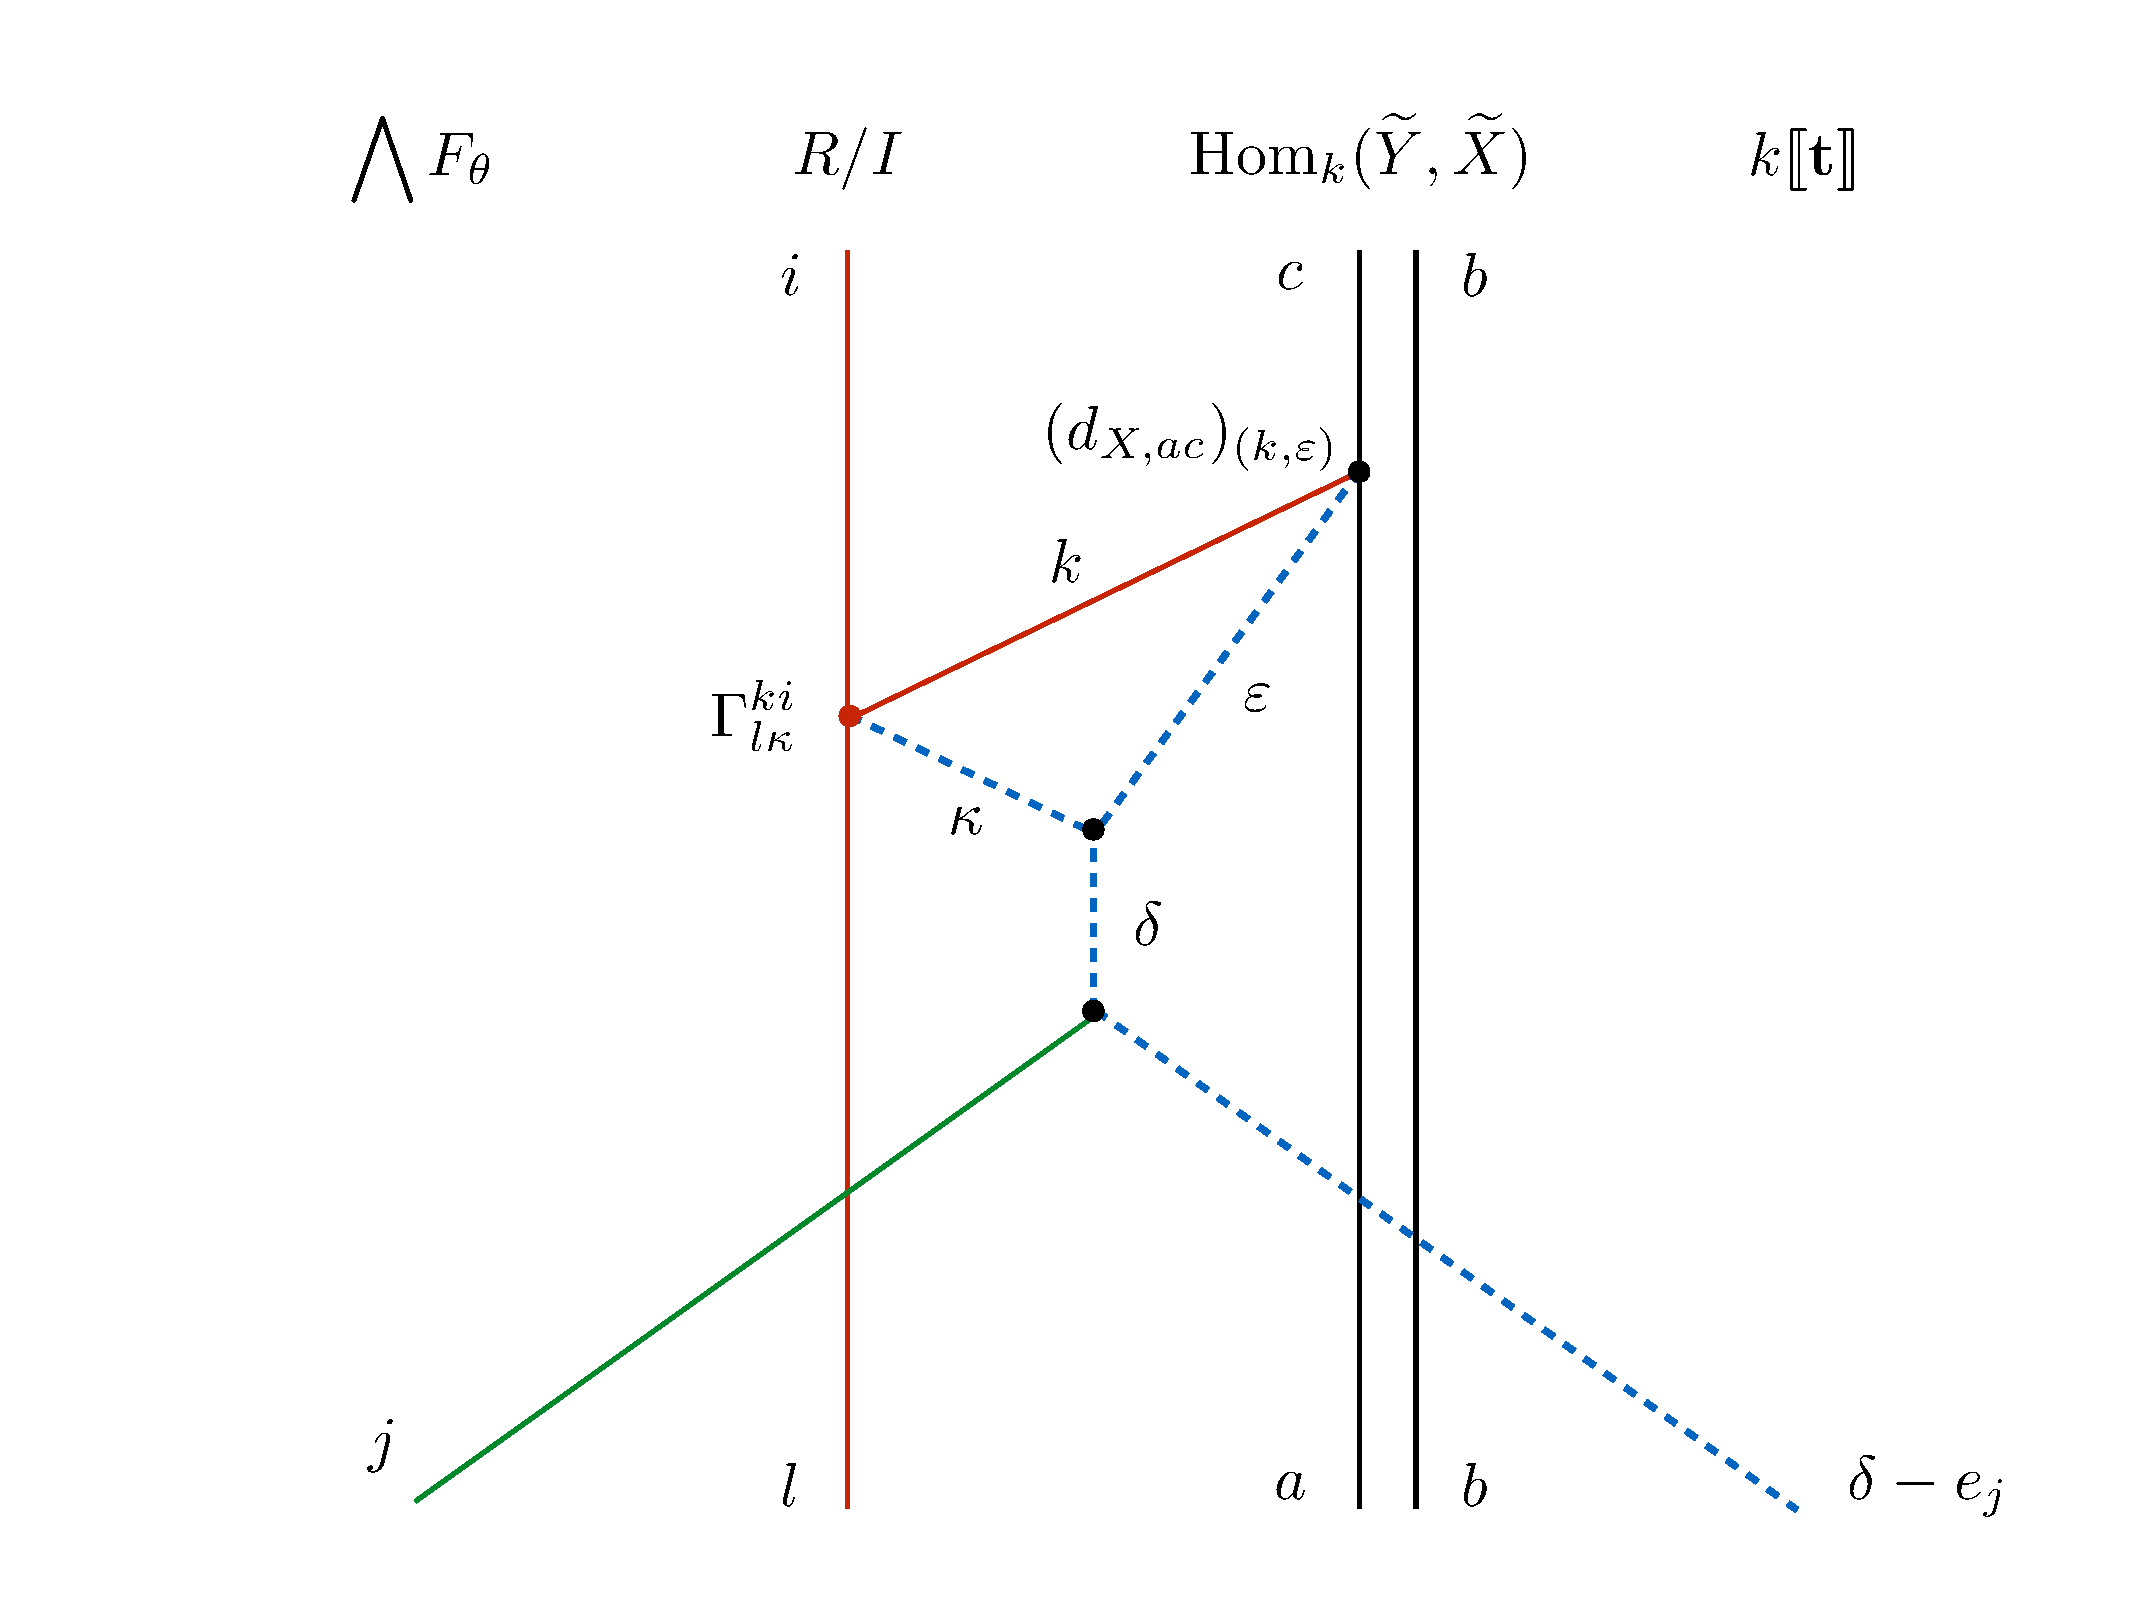
\includegraphics[scale=0.4]{dia15}
\end{center}

\begin{example} Let $W = y^d - x^d$ so that
\[
\md{A} = \bigwedge( k \psi_1^* \oplus k \psi_2^* ) = k \oplus k \psi_1^* \oplus k \psi_2^* \oplus k \psi_1^* \psi_2^*\,.
\]
I have only done the calculations for $d = 3$ but for general $d$ something similar should happen. One can see in the $d = 3$ case that the only nonzero multiplications are $r_2, r_3, r_4, r_6$. The calculation for $r_3$ is
\[
r_3( \Phi_0 \otimes \Phi_1 \otimes \Phi_2 ) = (-1)^{\sum_{i<j} \widetilde{\Phi}_i \widetilde{\Phi}_j}\Big( \prod_{i=0}^2 [\psi_2, \Phi_i] - \prod_{i=0}^2 [ \psi_1, \Phi_i ] \Big)\,.
\]
where $\widetilde{\Phi} = |\Phi| + 1$ is the degree in $\md{A}[1]$.

For $r_4$ and $r_6$ I know which operators contribute and their coefficients, but I don't yet have the signs correct. They are
\begin{align*}
r_4( \Phi_0 \otimes \cdots \otimes \Phi_3 ) &= \pm \frac{1}{2}\Big( [ \psi_2, \Phi_0] \cdot [ \psi_1, \Phi_1 ] \cdot [ \psi_1, [ \psi_2, \Phi_2 ] ] \cdot [ \psi_1, [ \psi_2, \Phi_3 ]] + \text{ cyclic rotations} \Big)\\
& \pm \Big( [ \psi_2, \Phi_0 ] \cdot [ \psi_1, [ \psi_2, \Phi_1 ] ] \cdot [ \psi_1, \Phi_2 ] \cdot [ \psi_1, [ \psi_2, \Phi_3 ]] + \text{ cyclic rotations} \Big)\,.
\end{align*}
and
\[
r_6( \Phi_0 \otimes \cdots \otimes \Phi_5 ) = \pm \frac{1}{4} \prod_{i=0}^5 [ \psi_1, [\psi_2, \Phi_i ]]\,.
\]
Here by a cyclic rotation I mean permute $\Phi_1, \Phi_2, \Phi_3$ in the first summand cyclically. I suspect this $A_\infty$-structure is cyclic with respect to the trace form that projects onto $k \psi_1^* \psi_2^*$ but I'm unable to check that at the moment.
\end{example}

\section{The proof}

\subsection{The homotopy retract}

Let $k$ be a characteristic zero field, $R =  k[x_1,\ldots,x_n]$ and let $W \in \mf{m}^3$ be a potential with chosen decomposition $W = \sum_{i=1}^n x_i W^i$. We aim to construct the minimal model of the following DG-algebra
\begin{align*}
\mathscr{A} &= \Big( \End_{R}(k^{\operatorname{stab}}), \; \partial = [d_{k^{\stab}},-] \; \Big)\\
&= \Big( R \otimes_k \End_k\Big( \bigwedge\big( \oplus_i k\psi_i \,\big) \Big),  \partial = \sum_i x_i [\psi_i^*,-] + \sum_i W^i [\psi_i,-] \;\Big)\,.
\end{align*}
Recall the module $\mathscr{H}$ of Definition \ref{defn:handop} which we recall here for the reader's convenience, writing $F = \oplus_i k \psi_i$ for compactness
\[
\mathscr{H} = R \otimes_k \bigwedge\big( \oplus_i k \theta_i \,\big) \otimes_k \End_k\Big( \bigwedge F \Big)\,.
\]
If we extend $\mathscr{A}$ by the exterior algebra on the $\theta$'s we get the DG-algebra
\[
\mathscr{A} \otimes_k \bigwedge\big( \oplus_i k\theta_i \,\big) = \big( \mathscr{H}, \partial \big)\,.
\]
The Koszul complex of the sequence $x_1,\ldots,x_n$ is
\be\label{eq:defnkoszulK}
K = \Big( R \otimes_k \bigwedge\big( \oplus_i k \theta_i \,\big), \; d_K = \sum_i x_i \theta_i^*\; \Big)
\ee
which may be extended by $\End_k\big( \bigwedge F \big)$ to give
\[
K \otimes_k \End_k\big( \bigwedge F \big) = \big( \mathscr{H}, d_K \big)\,.
\]

\begin{definition} The morphism of complexes $\pi: K \lto R/\mf{m}$ is defined by composing the projection of $K$ onto the submodule $R \cdot 1$ of $\theta$-degree zero forms, with the quotient $R \lto R/\mf{m}$. We also write $\pi$ for the following tensor product
\[
\xymatrix@C+2pc{
\big( \mathscr{H}, d_K + \partial \,\big) \ar[r]^-{\pi \otimes 1} & \Big( \End_k\big( \bigwedge F \big), 0 \,\Big)\,.
}
\]
where we use that $R/\mf{m} \otimes_R \End_R(k^{\stab})$ has zero differential by the hypothesis that $W \in \mf{m}^2$. 
\end{definition}

\begin{definition} We write $\sigma$ for the inclusion $\End_k\big( \bigwedge F \big) \lto \mathscr{H}$ defined by
\[
\sigma( \Phi ) = 1 \otimes 1 \otimes \Phi\,.
\]
\end{definition}

\begin{definition}\label{defn:lpsi} Let $L_{\psi_i}$ denote the odd operator on $\End_k\big( \bigwedge F \big)$ defined by
\[
L_{\psi_i}( \alpha ) = \psi_i \circ \alpha = (\psi_i \wedge (-)) \circ \alpha\,,
\]
so that $L_{\psi_i}(\alpha)(x) = \psi_i \wedge \alpha(x)$.
\end{definition}

Throughout $\sum_i$ stands for $\sum_{i=1}^n$.

\begin{theorem}\label{theorem:main_retract} Using the following even homogeneous operators on $\mathscr{H}$,
\be
\delta = \sum_i L_{\psi_i} \theta_i^*\,, \qquad \sigma_\infty = \sum_{m \ge 0} (-1)^m (H \partial)^m \sigma\,,\label{eq:sigmainftyorig}
\ee
and the following odd homogeneous operators
\begin{gather}
\partial = \sum_i x_i [\psi_i^*,-] + \sum_i W^i [\psi_i,-]\,,\\
\nabla = \sum_i \partial_i \theta_i\,, \qquad H = [d_K, \nabla]^{-1} \nabla\,,\label{defn:Horiginal}\\
H_\infty = \sum_{m \ge 0} (-1)^m (H \partial)^m H\,.\label{eq:hinftyorig}
\end{gather}
there is a diagram of $k$-linear homotopy equivalences
\be\label{eq:first_he}
\xymatrix@C+3pc{
\big( \mathscr{H}, \partial \,\big) \ar@<1ex>[r]^-{\exp(-\delta)} & \big( \mathscr{H}, d_K + \partial \,\big) \ar@<1ex>[l]^-{ \exp(\delta) } \ar@<1ex>[r]^-{\pi} & \Big( \End_k\big( \bigwedge F \big), 0 \,\Big)\,.\ar@<1ex>[l]^-{ \sigma_\infty }
}
\ee
More precisely, $\exp(-\delta), \exp(\delta)$ are mutually inverse as $k$-linear maps, $\pi \circ \sigma_\infty = 1$ and
\be
1_{\mathscr{H}} - \big[ d_K + \partial, H_\infty \big] = \sigma_\infty \circ \pi\,.
\ee
\end{theorem}
\begin{proof}
For the duration of the proof let $\mathscr{E} = \End_k\big( \bigwedge F \big)$. It is easy to check that $\exp(\delta),\exp(-\delta)$ intertwines the differentials $\partial$ and $d_K + \partial$ and therefore gives an isomorphism between the first two complexes in \eqref{eq:first_he} \cite[Proposition 4.11]{murfet}. The operator $\psi_j = \psi_j \wedge -$ on $k^{\stab}$ satisfies
\[
[ \psi_j, d_{k^{\stab}} ] = \big[ \psi_j, \sum_i x_i \psi_i^* \big] = x_j \cdot 1\,.
\]
That is, $\psi_j$ is a homotopy for the action of $x_j$ on $k^{\stab}$. It is then easy to check that the odd operator $\alpha \mapsto \psi_j \circ \alpha$ on $\End_R(k^{\stab})$ is also a homotopy for $x_j$.
\end{proof}

It is the homotopy retract \eqref{eq:first_he} that we will ultimately feed into the minimal model theorem, taking as our DG-algebra $(\mathscr{H}, \partial)$ equipped with the projection $\pi \exp(-\delta)$ injection $\exp(\delta) \sigma_\infty$ and the homotopy $\exp(\delta) H_\infty \exp(-\delta)$. In broad outlines, these operators lead to the three types of Feynman diagram interactions as follows:
\begin{itemize}
\item A-type interactions arise from $H_\infty$, more precisely the $H \partial$ factors.
\item B-type interactions arise from the ``odd man out'' $H$ at the right end of $H_\infty$.
\item C-type interactions arise from $\exp(\pm \delta)$.
\end{itemize}
We address each of these in turn before, in Section \ref{??}, finishing the proof.

\subsection{Deriving A-type and B-type interactions}

The A-type and B-type interactions arise from $\sigma_\infty$ and $H_\infty$ from \eqref{eq:sigmainftyorig},\eqref{eq:hinftyorig}. The main task is to understand $(H \partial)^m$. We have for $m > 0$, as an operator on $\mathscr{H}$
\begin{align*}
\big( H \partial )^m &= \prod_{i=1}^m \sum_{j_i = 1}^n H \circ \Big( x_{j_i} [\psi_{j_i}^*,-] + W^{j_i} [\psi_{j_i},-] \Big)\,.
\end{align*}
Prior to Definition \ref{defn:otc} we observed that in calculating $\langle D_{T,C} \rangle$ it suffices to consider operators on the $\nZ_2$-graded $k$-module of $\mathscr{H}$ given by
\be
\mathscr{H}' = R \otimes_k \bigwedge\big( \oplus_{i=1}^n k \theta_i \,\big) \otimes_k \mathscr{B}\,.
\ee
In the next lemma we calculate $(H \partial)^m$ on $\mathscr{H} \cap \Ker(\nabla)$, where $\nabla = \sum_i \partial_i \theta_i$. Before we do this we introduce some notation: in the calculation we use a $\nZ$-grading on $\mathscr{H}'$ defined as follows: $\mathscr{H}'_a$ is the $k$-submodule spanned by tensors of the form
\begin{align*}
f \otimes \omega \otimes \kappa \text{ where } f \in R\,, \omega \in \bigwedge( \oplus_i k \theta_i ), \kappa \in \mathscr{B} \text{ and } |f|_{\nZ} + |\omega|_{\nZ} = a\,.
\end{align*}
Here $|-|_{\nZ}$ denotes the $\nZ$-grading with $|x_i|_{\nZ} = 1$ and $|\theta_i|_{\nZ} = 1$. To be perfectly clear: we have $|\theta_1 \theta_2|_{\nZ} = 2$, as compared to $| \theta_1 \theta_2 | = 0$ in the $\nZ_2$-grading used elsewhere in the text.

\begin{lemma}\label{lemma:commutator_numberop} If $f \in R$ and $\omega \in \bigwedge( \oplus_{i=1}^n k \theta_i )$ are homogeneous then
\be
[d_K, \nabla]( f \otimes \omega ) = ( |f|_{\nZ} + |\omega|_{\nZ} ) f \otimes \omega\,.
\ee
\end{lemma}

\begin{proposition}\label{prop:hpartialmrestrict} Restricted to $\mathscr{H}'_a \cap \Ker(\nabla)$, $(H \partial)^m$ is equal to
\be\label{eq:hpartialmrestrict}
\sum_{\substack{1 \le j_1 < \cdots < j_m \le n \\ 1 \le z_1 < \cdots < z_m \le n \\ \gamma_1,\ldots,\gamma_m \in \mathbb{N}^n \setminus \{0\}}} \sum_{\nu \in \mathfrak{S}_m} \frac{\zeta_{a}( |\gamma_1|,\ldots,|\gamma_m| )}{|\gamma_1| \cdots |\gamma_m|} \prod_{i=1}^m W^{j_i}(\gamma_i) \partial_{z_{\nu(i)}}(x^{\gamma_i}) \theta_{z_{\nu(i)}} [ \psi_{j_i}, - ]\,.
\ee
\end{proposition}
\begin{proof}
On this submodule of $\mathscr{H}$ the operators $[\psi_i^*,-]$ act as zero, and so $(H \partial)^m$ takes a simpler form. If $\underline{j}$ ranges over sequences of length $m$ in $\{1,\ldots,n\}^m$ and $\underline{\gamma}$ over sequences of length $m$ in $\mathbb{N}^n$ then
\begin{align*}
\big( H \partial )^m \arrowvert_{\mathscr{H}'} &= \sum_{\underline{j}} \prod_{i=1}^m H \circ \Big( W^{j_i} [ \psi_{j_i}, - ] \Big)\\
&= \sum_{\underline{j}} \prod_{i=1}^m H \circ \Big( \sum_{\gamma_i} W^{j_i}(\gamma_i) x^{\gamma_i} [ \psi_{j_i}, - ] \Big)\\
&= \sum_{\underline{j}, \underline{\gamma}} \prod_{i=1}^m H \circ \Big( W^{j_i}(\gamma_i) x^{\gamma_i} [ \psi_{j_i}, - ] \Big)\\
&= \sum_{\underline{j}, \underline{\gamma}} \prod_{i=1}^m [d_K, \nabla]^{-1} \nabla \circ \Big( W^{j_i}(\gamma_i) x^{\gamma_i} [ \psi_{j_i}, - ] \Big)\,.
\end{align*}
Note that $W^i$ contains no constant term, since by hypothesis $W \in \mf{m}^2$, so in fact we may assume that all $\gamma_i$ are nonzero. Our convention is that products of operators expand from left to right as $i$ increases. Lemma \ref{lemma:commutator_numberop}

Now we consider the scalar factors produced by the $[d_K, \nabla]^{-1}$ when we apply $(H \partial)^m$ to a tensor $f \otimes \omega \otimes \Psi$. Observe how the sum of the polynomial and $\theta$-degree changes with each application of $H \partial$. Multiplying with $x^{\gamma_i}$ increases the polynomial degree by $|\gamma_i|$, while applying $\nabla$ decreases the polynomial degree and increases the $\theta$-degree by one, so overall the $i$th copy of $H \partial$ (reading from left to right) increases the sum of the two degrees from
\[
|f|_{\nZ} + |\omega|_{\nZ} + \sum_{t > i} |\gamma_t| \qquad \text{ to } \qquad |f|_{\nZ} + |\omega|_{\nZ} + \sum_{t \ge i} |\gamma_t|\,.
\]
If we write $a = |f| + |\omega|$ then the scalar factor contributed by the copies of $[d_K, \nabla]^{-1}$ in $(H \partial)^m$ applied to $f \otimes \omega \otimes \Psi$ is therefore
\[
\frac{1}{(a + |\gamma_m|)(a + |\gamma_m| + |\gamma_{m-1}|) \cdots (a + |\gamma_m| + \cdots + |\gamma_1|)}\,.
\]
This leads us to the un-symmetrised version of $\zeta$ from Definition \ref{defn:zeta}: given a sequence $a_1,\ldots,a_m \ge 1$ of integers and $a \ge 0$ we define
\be\label{defn:zeta_unsym}
\zeta'_a(a_1,\ldots,a_m) = \frac{1}{(a + a_m)(a + a_{m-1} + a_m) \cdots (a + a_1 + \cdots + a_m)}\,.
\ee
Let $\mathscr{H}'_a \subseteq \mathscr{H}'$ denote the submodule of elements of degree $a$, when we take the $\nZ$-grading induced by the usual $\nZ$-grading on $R$ and the exterior algebra in the $\theta$'s (so, the grading does not count $\psi$'s). Then we have computed that
\be
(H \partial)^m|_{\mathscr{H}'_a} = \sum_{\underline{j}, \underline{\gamma}} \zeta'_{a}( |\gamma_1|, \ldots, |\gamma_m| ) \prod_{i=1}^m \nabla \circ \big( W^{j_i}(\gamma_i)x^{\gamma_i} [ \psi_{j_i}, - ] \big) \,.
\ee
For a $k$-linear operator $T$ and an element $x \in \Ker(\nabla)$ since $\nabla^2 = 0$ we have
\[
\nabla T \cdots \nabla T (x) = [\nabla, T] \cdots [\nabla, T](x)\,.
\]
Using $[ \nabla, f ] = \sum_q \partial_q(f) \theta_q$ we therefore have
\begin{align*}
\big( H \partial )^m|_{\mathscr{H}'_a \cap \Ker(\nabla)} &= \sum_{\underline{j}, \underline{\gamma}} \zeta'_{a}( |\gamma_1|, \ldots, |\gamma_m| ) \prod_{i=1}^m \Big[ \nabla, W^{j_i}(\gamma_i)x^{\gamma_i} [ \psi_{j_i}, - ] \Big]\\
&= \sum_{\underline{j}, \underline{\gamma},\underline{z}} \zeta'_{a}( |\gamma_1|, \ldots, |\gamma_m| ) \prod_{i=1}^m W^{j_i}(\gamma_i) \partial_{z_i}(x^{\gamma_i}) \theta_{z_i} [ \psi_{j_i}, - ]
\end{align*}
where $\underline{j},\underline{z}$ both range over $\{1, \ldots, n\}^m$. Since $[ \psi_j, - ]^2 = 0$ the only nonzero contributions are from sequences $\underline{j} = (j_1,\ldots,j_m)$ without repeats and similarly for $\underline{z}$. Thus
\begin{align*}
&= \sum_{\substack{j_1 < \cdots < j_m \\ z_1 < \cdots < z_m}} \sum_{\rho,\nu \in \mathfrak{S}_m} \sum_{\underline{\gamma}} \zeta'_{a}( |\gamma_1|, \ldots, |\gamma_m| ) \prod_{i=1}^m W^{j_{\rho(i)}}(\gamma_i) \partial_{z_{\nu(i)}}(x^{\gamma_i}) \theta_{z_{\nu(i)}} [ \psi_{j_{\rho(i)}}, - ]\\
&= \sum_{\substack{j_1 < \cdots < j_m \\ z_1 < \cdots < z_m}} \sum_{\rho,\nu \in \mathfrak{S}_m} \sum_{\underline{\gamma}} \zeta'_{a}( |\gamma_1|, \ldots, |\gamma_m| ) \prod_{i=1}^m W^{j_i}(\gamma_{\rho^{-1}(i)}) \partial_{z_{\nu\rho^{-1}(i)}}(x^{\gamma_{\rho^{-1}(i)}}) \theta_{z_{\nu\rho^{-1}(i)}} [ \psi_{j_i}, - ]\\
&= \sum_{\substack{j_1 < \cdots < j_m \\ z_1 < \cdots < z_m}} \sum_{\rho,\nu \in \mathfrak{S}_m} \sum_{\underline{\gamma}} \zeta'_{a}( |\gamma_{\rho(1)}|, \ldots, |\gamma_{\rho(m)}| ) \prod_{i=1}^m W^{j_i}(\gamma_i) \partial_{z_{\nu(i)}}(x^{\gamma_i}) \theta_{z_{\nu(i)}} [ \psi_{j_i}, - ]\\
&= \sum_{\substack{j_1 < \cdots < j_m \\ z_1 < \cdots < z_m}} \sum_{\nu \in \mathfrak{S}_m} \sum_{\underline{\gamma}} \frac{\zeta_{a}( |\gamma_1|,\ldots,|\gamma_m| )}{|\gamma_1| \cdots |\gamma_m|} \prod_{i=1}^m W^{j_i}(\gamma_i) \partial_{z_{\nu(i)}}(x^{\gamma_i}) \theta_{z_{\nu(i)}} [ \psi_{j_i}, - ]
\end{align*}
%That is, if we write
%\[
%Y = \{ ( z, \gamma ) \l 1 \le z \le n\,, \gamma \in \mathbb{N}^m\,, \gamma_z \ge 1 \}
%\]
%then
as claimed.
\end{proof}

\begin{remark} Since $\nabla \sigma = 0$ and $\nabla^2 = 0$ the proposition applies to calculate $\sigma_\infty, H_\infty$. In the former case we simply append $\sigma$ and use \eqref{eq:sampzero} to see that $(H \partial)^m \sigma$ is given under the same summation over $\underline{j},\underline{z},\underline{\gamma}, \nu$ as in \eqref{eq:hpartialmrestrict} by
\be
\sum_{\underline{j},\underline{z},\underline{\gamma},\nu} \frac{1}{|\gamma_1| \cdots |\gamma_m|} \Big\{ \prod_{i=1}^m W^{j_i}(\gamma_i) \partial_{z_{\nu(i)}}(x^{\gamma_i}) \theta_{z_{\nu(i)}} [ \psi_{j_i}, - ] \Big\} \circ \sigma\,.
\ee
In the case of $H_\infty$ we observe that $H = [d_K, \nabla]^{-1} \nabla$ sends $\mathscr{H}'_a$ into $\mathscr{H}'_a \cap \Ker(\nabla)$, and we have that $(H \partial)^m H$ on $\mathscr{H}'_a$ is given by
\be
\sum_{\underline{j},\underline{z},\underline{\gamma},\nu} \sum_{t = 1}^n \frac{1}{a} \frac{\zeta_{a}( |\gamma_1|,\ldots,|\gamma_m| )}{|\gamma_1| \cdots |\gamma_m|} \Big\{ \prod_{i=1}^m W^{j_i}(\gamma_i) \partial_{z_{\nu(i)}}(x^{\gamma_i}) \theta_{z_{\nu(i)}} [ \psi_{j_i}, - ] \Big\} \circ \partial_t \theta_t\,.
\ee
\end{remark}

\begin{remark}\label{remark:virt_part_2} Continuing from Remark \ref{remark:virtual_part} we note that in contrast to the way we usually think about the minimal model construction in the setting of topological string theory \cite{??} the elements $\Psi$ of $\mathscr{B}$ are not immediately identified with cohomology classes of $\mathscr{B}$. 

Of course $\sigma_\infty(\Psi)$ is a cycle for $\partial$, but this is already given by a complicated sum which contributes multiple Feynman diagrams in the calculus of Definition \ref{??}. That is to say, we have found it useful for purposes of calculation to have the incoming states in our Feynman diagrams to be elements of $\mathscr{H}$ that are \emph{not} cycles. Note that as we vary the potential $W$ the elements of $\mathscr{H}$ that are cycles will change - this makes it awkward to take as a starting point the cohomology of $\mathscr{H}$. In our approach the subspace $\mathscr{B}$ remains fixed, and even in the case of quadratic terms it is only the projection to $\mathscr{B}$ that changes.
\end{remark}

\subsection{Deriving C-type interactions}
% see ainfmf4

Let us briefly recall some of the notation from earlier: we write $F = \oplus_i k \psi_i$ and use the operators $L_{\psi_i}$ of Definition \ref{defn:lpsi} and $\delta$ of \eqref{eq:sigmainftyorig}. We set $\delta_i = L_{\psi_i} \theta_i^*$ so that $\delta = \sum_i \delta_i$. To be explicit, given $\omega_i \in \bigwedge( \oplus_i k \theta_i )$ and $\kappa_i \in \End_k(\bigwedge F)$
\[
\delta_i( \omega \otimes \kappa ) = L_{\psi_i}\big( \theta_i^*( \omega ) \otimes \kappa ) = (-1)^{|\omega| + 1} \theta_i^*(\omega) \otimes \psi_i \circ \kappa\,.
\]

\begin{lemma}\label{lemma:stratos} For $1 \le i \le n$ there is a commutative diagram
\be
\xymatrix@C+3pc@R+1pc{
\mathscr{H} \otimes_k \mathscr{H} \ar[d]_-{\delta_i \otimes 1 + 1 \otimes \delta_i + [\psi_i,-] \otimes \theta_i^*} \ar[r]^-{m_2} & \mathscr{H} \ar[d]^-{\delta_i}\\
\mathscr{H} \otimes_k \mathscr{H} \ar[r]_-{m_2} & \mathscr{H}
}
\ee
\end{lemma}
\begin{proof}
By direct calculation: given $\omega_j \in \bigwedge( \oplus_i k \theta_i )$ and $\kappa_j \in \bigwedge( \oplus_i k \psi_i )$
\begin{align*}
&m_2\big( \delta_i \otimes 1 + 1 \otimes \delta_i \big)( \omega_1 \otimes \kappa_1 \otimes \omega_2 \otimes \kappa_2 )\\
&= m_2\big( \delta_i( \omega_1 \otimes \kappa_1 ) \otimes \omega_2 \otimes \kappa_2 \big)\\
&+ m_2\big( \omega_1 \otimes \kappa_1 \otimes \delta_i( \omega_2 \otimes \kappa_2 ) \big)\\
&= (-1)^{|\omega_1| + 1}m_2\big( \theta_i^*(\omega_1) \otimes \psi_i \circ \kappa_1 \otimes \omega_2 \otimes \kappa_2 )\\
&+ (-1)^{|\omega_2| + 1}m_2\big( \omega_1 \otimes \kappa_1 \otimes \theta_i^*(\omega_2) \otimes \psi_i \circ \kappa_2 \big)\\
&= (-1)^{|\omega_1|+1+(|\kappa_1|+1)|\omega_2|} \theta_i^*(\omega_1) \omega_2 \otimes \psi_i \circ \kappa_1 \circ \kappa_2\\
&+ (-1)^{|\omega_2|+1+(|\omega_2|+1)|\kappa_1|} \omega_1 \theta_i^*(\omega_2) \otimes \kappa_1 \circ \psi_i \circ \kappa_2
\end{align*}
Similarly one computes
\begin{align*}
&m_2 \big( [\psi_i,-] \otimes \theta_i^* \big)( \omega_1 \otimes \kappa_1 \otimes \omega_2 \otimes \kappa_2 \big)\\
&= (-1)^{|\kappa_1|} m_2 \big( \omega_1 \otimes [\psi_i, \kappa_1] \otimes \theta_i^*(\omega_2) \otimes \kappa_2 \big)\\
&= (-1)^{|\kappa_1|+(|\kappa_1|+1)(|\omega_2|+1)} \omega_1 \theta_i^*(\omega_2) \otimes [\psi_i, \kappa_1] \circ \kappa_2\,.
\end{align*}
Adding these together yields that $\delta_i \otimes 1 + 1 \otimes \delta_i + [\psi_i,-] \otimes \theta_i^*$ on $\omega_1 \otimes \kappa_1 \otimes \omega_2 \otimes \kappa_2$ is
\begin{align*}
&= (-1)^{|\omega_1|+1+(|\kappa_1|+1)|\omega_2|} \theta_i^*(\omega_1) \omega_2 \otimes \psi_i \circ \kappa_1 \circ \kappa_2\\
&+ (-1)^{|\kappa_1|+(|\kappa_1|+1)(|\omega_2|+1)} \omega_1 \theta_i^*(\omega_2) \otimes \psi_i \circ \kappa_1 \circ \kappa_2\\
&= (-1)^{|\omega_1|+|\omega_2|+|\kappa_1||\omega_2|+1} \theta_i^*( \omega_1 \omega_2 ) \otimes \psi_i \circ \kappa_1 \circ \kappa_2\\
&= (-1)^{|\kappa_1||\omega_2|}\delta_i\big( \omega_1 \omega_2 \otimes \kappa_1 \circ \kappa_2 \big)\\
&= \delta_i \circ m_2\big( \omega_1 \otimes \kappa_1 \otimes \omega_2 \otimes \kappa_2 \big)
\end{align*}
as claimed.
\end{proof}

\begin{definition} We define $\Xi_i = [ \psi_i, - ] \otimes \theta_i^* : \mathscr{H}^{\otimes 2} \lto \mathscr{H}^{\otimes 2}$ and $\Xi = \sum_i \Xi_i$. 
\end{definition}

\begin{lemma}\label{lemma:somecommt} As operators on $\mathscr{H} \otimes_k \mathscr{H}$, for all $1 \le i,j \le n$
\begin{align}
\big[ \delta_i \otimes 1, 1 \otimes \delta_j \big] &= 0\\
\big[ \delta_i \otimes 1, \Xi_j \big] &= 0\\
\big[ 1 \otimes \delta_i, \Xi_j \big] &= 0\,.
\end{align}
\end{lemma}

\begin{proposition}\label{prop:adamant} There is a commutative diagram
\be
\xymatrix@C+3pc@R+2pc{
\mathscr{H} \otimes \mathscr{H} \ar[d]_-{\exp(-\delta) \otimes \exp(-\delta)} \ar[r]^-{m_2} & \mathscr{H} \ar[dd]^-{\exp(-\delta)}\\
\mathscr{H} \otimes \mathscr{H} \ar[d]_-{\exp(-\Xi)}\\
\mathscr{H} \otimes \mathscr{H} \ar[r]_-{m_2} & \mathscr{H}
}
\ee
\end{proposition}
\begin{proof}
By Lemma \ref{lemma:somecommt} we have
\[
\exp\big(-\big[ \delta_i \otimes 1 + 1 \otimes \delta_i + \Xi_i \big]\big) = \exp(-\Xi_i) \circ \big\{ \exp(-\delta_i) \otimes \exp(-\delta_i) \big\}
\]
and therefore
\[
\exp\big(-\big[ \delta \otimes 1 + 1 \otimes \delta + \Xi \big]\big) = \exp(-\Xi) \circ \big\{ \exp(-\delta) \otimes \exp(-\delta) \big\}\,.
\]
By Lemma \ref{lemma:stratos} then
\begin{align*}
\exp(-\delta) m_2 &= \sum_{m \ge 0} (-1)^m \frac{1}{m!} \delta^m m_2\\
&= \sum_{m \ge 0} (-1)^m \frac{1}{m!} m_2 \big\{ \delta \otimes 1 + 1 \otimes \delta + \Xi \big\}^m\\
&= m_2 \exp\big(-\big[ \delta \otimes 1 + 1 \otimes \delta + \Xi \big] \big)\\
&= m_2 \exp(-\Xi) \circ \big\{ \exp(-\delta) \otimes \exp(-\delta) \big\}\,,
\end{align*}
which completes the proof.
%Immediately from \eqref{eq:graded_jacobi} and \eqref{eq:wedge_contract_comm} we have
%\begin{align*}
%\big[ [ \varepsilon_i^*, -], \varepsilon_j \big] &= \big[ [ \varepsilon_i, - ], \varepsilon_j^* \big] = \delta_{ij} \cdot 1\,.\\
%\big[[ \varepsilon_i^*, -], \varepsilon_j^* \big] &= \big[[\varepsilon_i, -], \varepsilon_j\big] = 0\,.
%\end{align*}
\end{proof}

Observe finally that
% see ainfmf9 p.14
\be
\exp(-\Xi) = \sum_{m \ge 0} (-1)^m \sum_{1 \le j_1 < \cdots < j_m \le n} \prod_{i=1}^m \;[\psi_{j_i},-] \otimes \theta_{j_i}^*\,.
\ee

\subsection{Putting it all together}

In this section we put together all the earlier elements, and prove the description of the minimal model of $\mathscr{A}$ given in Section \ref{??}. In this section we write
\[
\mathscr{E} = \End_k\Big( \bigwedge( \oplus_i k \psi_i ) \Big)\,.
\]
The starting point is Theorem \ref{theorem:main_retract}, which gives us a strong deformation retract
\be\label{eq:ho_retract_for_mm}
\xymatrix@C+5pc{
\big( \mathscr{H}, \partial \,\big) \ar@<1ex>[r]^-{\pi\exp(-\delta)} & \big( \mathscr{E}, 0 \big) \ar@<1ex>[l]^-{ \exp(\delta)\sigma_\infty }
}
\ee
with $\pi \exp(-\delta) \circ \exp(\delta) \sigma_\infty = 1$ and
\[
\exp(\delta)\sigma_\infty \pi\exp(-\delta) = 1 - \big[ \partial, \exp(\delta) H_\infty \exp(-\delta) \big]\,.
\]

\begin{definition} Let $\xi_q$ denote the product $\xi_q: \mathscr{E}[1]^{\otimes q} \lto \mathscr{E}[1]$ induced by the homotopy retract \eqref{eq:ho_retract_for_mm} and the minimal model construction, defining an $A_\infty$-structure on $\mathscr{E}$. That is,
\[
\xi_q = \sum_{T \in \cat{T}_q} (-1)^{e_i(T)} \langle D_T \rangle
\]
where $D_T$ is the decoration given by the assignment of modules
\begin{itemize}
\item $\mathscr{E}$ to each leaf including the root, and
\item $\mathscr{H}$ to each edge.
\end{itemize}
To each vertex $v$ of $A(T)$ we associate an operator $\phi_v$ as follows:
\begin{itemize}
\item if $v$ is an input, then $\phi_v = \exp(\delta)\sigma_\infty$.
\item if $v$ comes from an internal edge of $T$, then $\phi_v = \exp(\delta)H_\infty\exp(-\delta)$.
\item if $v$ comes from an internal vertex of $T$, then $\phi_v = r_2$ where $r_2$ is the forward suspension of the product $m_2$ in $\mathscr{H}$, that is,
\be\label{eq:r2vsm2}
r_2( \alpha \otimes \beta ) = (-1)^{\widetilde{\alpha}\widetilde{\beta} + \widetilde{\beta} + 1} m_2( \beta \otimes \alpha )\,.
\ee
\item if $v$ is the root, then $\phi_v = \pi \exp(-\delta)$.
\end{itemize}
\end{definition}

\begin{proposition} For $q \ge 2$
\be
\xi_q( \Lambda_q, \ldots, \Lambda_1 ) = \sum_{T \in \cat{T}_q} (-1)^{Q(T, \Lambda_1, \ldots, \Lambda_q)} \langle D'_T \rangle( \Lambda_1,\ldots,\Lambda_q)
\ee
where $Q(T, \Lambda_1, \ldots, \Lambda_q)$ is as in \eqref{eq:defnQsign}, and $D'_T$ is the decoration of $A(T)$ assigning $\mathscr{E}$ to each leaf and $\mathscr{H}$ to each edge, and to each vertex $v$ the operator $\phi_v$ defined as follows:
\begin{itemize}
\item if $v$ is an input, then $\phi_v = \sigma_\infty$.
\item if $v$ comes from an internal edge of $T$, then $\phi_v = H_\infty$.
\item if $v$ comes from an internal vertex of $T$, then
\[
\phi_v = m_2 \circ \exp(- \Xi)\,.
\]
\item if $v$ is the root, then $\phi_v = \pi$.
\end{itemize}
\end{proposition}
\begin{proof}
The substitution of $m_2$ for $r_2$ incurs some sign factors and reverses the order of the inputs, and we will return to this sign at the end. We prove the proposition by taking the ``extra'' $\exp(-\delta)$ factor at the root and moving it upwards in the tree: at the vertex $v$ adjacent to the root, we use Proposition \ref{prop:adamant} to see that
\[
\exp(-\delta) \circ m_2 = m_2 \circ \exp(-\Xi) \circ (\exp(-\delta) \otimes \exp(-\delta))\,,
\]
which replaces the $m_2$ at the vertex by $m_2 \circ \exp(-\Xi)$ and propagates the $\exp(-\delta)$ factors to the edges adjacent and above $v$.  internal this extra factor has the effect of
\[
\exp(-\delta) \circ \exp(\delta) H_\infty \exp(-\delta) = H_\infty \exp(-\delta)
\] 
leaving behind a $H_\infty$ and moving upwards, while in the case of an external edge
\[
\exp(-\delta) \circ \exp(\delta) \sigma_\infty = \sigma_\infty
\]
we are left with a bare $\sigma_\infty$.

Now to return to the signs, which come from \eqref{eq:r2vsm2} applied at every internal vertex of $T$, when evaluating $\xi_q( \Lambda_q, \ldots, \Lambda_1 )$. The labels $\exp(\delta) H_\infty \exp(-\delta)$ and $r_2$ on internal edges and vertices have degree $+1$ with respect to the tilde grading, which means that when a $\Lambda_i$ reaches an internal vertex of $T$ it is still carrying the same tilde grading $\widetilde{\Lambda_i}$.

It follows that the $\widetilde{\alpha}\widetilde{\beta}$ part of $\eqref{eq:r2vsm2}$ contributes overall $\sum_{i < j} \widetilde{\Lambda_i} \widetilde{\Lambda_j}$ while the $\widetilde{\beta}$ part contributes $\sum_i \widetilde{\Lambda_i} C_i$, and the $1$ contributes $q - 1$, the number of internal vertices.
\end{proof}

\subsection{The minimal model}

Following ainfcat2 let $Q$ be the commutative associative (but possibly non-unital) denoted $R_A$ on p.3 ainfcat2 and let us write
\be
\HH = \bigoplus_{Y,X \in \operatorname{ob}(\CC)} \bigwedge F_\theta \otimes_k \Hom_R(Y,X) \otimes_R \widehat{R}
\ee
with its $Q$-bimodule structure and with forward suspended operations
\[
r_k: \HH[1]^{\otimes_Q k} \lto \HH[1]
\]
Then p.9 ainfcat2 produces the $k$-linear $Q$-bilinear maps
\[
\rho_k = \sum_{T \in \cat{T}_k} \rho_T \in \Hom_{{}_Q \operatorname{Mod}_Q}( B[1]^{\otimes_Q k}, B[1] )
\]
where $B = Im(P) \subseteq \HH$ identified with the relevant direct sum of quotients as in \eqref{eq_6_2}.

\begin{definition} For $1 \le i \le n$ we define the odd $\widehat{R}$-linear, $Q$-bilinear operators
\[
\lambda_i, \theta_i^*: \HH \lto \HH
\]
by the formulas
\[
\lambda_i = \sum_{Y,X} \lambda_i^{Y,X}\,, \qquad \theta_i^* = \sum_{Y,X} \theta_i^*\,.
\]
We set $\delta = \sum_{i=1}^n \delta_i$ with $\delta_i = \lambda_i \theta_i^* = \sum_{Y,X} \lambda^{Y,X}_i \theta_i^*$.
\end{definition}

\begin{definition} For $1 \le i \le n$ we define the odd $\widehat{R}$-linear $Q$-bilinear operators $[\lambda_i, -]: \HH \lto \HH$ defined on $\omega \otimes \alpha \in \bigwedge F_\theta \otimes_k \Hom_R(Y,X) \otimes_R \widehat{R}$ by
\[
[\lambda_i,-](\omega \otimes \alpha) = (-1)^{|\omega|} \omega \otimes \big\{ \lambda_i^X \circ \alpha - (-1)^{|\alpha|} \alpha \circ \lambda_i^Y \big\}.
\]
\end{definition}

\begin{lemma}\label{lemma_p_9} For $1 \le i \le n$ the following diagram commutes
\be
\xymatrix@C+3pc@R+1pc{
\mathscr{H}[1] \otimes_Q \mathscr{H}[1] \ar[d]_-{\delta_i \otimes 1 + 1 \otimes \delta_i - \theta_i^* \otimes [\lambda_i,-]} \ar[r]^-{r_2} & \mathscr{H}[1] \ar[d]^-{\delta_i}\\
\mathscr{H}[1] \otimes_Q \mathscr{H}[1] \ar[r]_-{r_2} & \mathscr{H}[1]
}
\ee
\end{lemma}
\begin{proof}
Note that $r_2( x_2 \otimes x_1 ) = (-1)^{\widetilde{x_1}\widetilde{x_2} + \widetilde{x_1} + 1} x_1 \circ x_2$ where the tilde grading is as in Definition \ref{defn:tildegrading} and $x_1 \circ x_2$ denotes ordinary composition. We may choose objects $X,Y,Z$ and check commutativity of the diagram on a tensor $(\omega_2 \otimes x_2) \otimes (\omega_1 \otimes x_1)$ for vectors
\[
\omega_1,\omega_2 \in \bigwedge F_\theta \,, \qquad x_1 \in \Hom_R(Y,X)\,, x_2 \in \Hom_R(Z,Y)\,.
\]
We calculate
\begin{align*}
r_2( \delta_i \otimes 1 &+ 1 \otimes \delta_i )\big( (\omega_2 \otimes x_2) \otimes (\omega_1 \otimes x_1) \big)\\
&= r_2 \big( \lambda_i( \theta_1^* \omega_2 \otimes x_2 ) \otimes \omega_1 \otimes x_1 + \omega_2 \otimes x_2 \otimes \lambda_i( \theta_1^* \omega_1 \otimes x_1) \big)\\
&= r_2 \big( (-1)^{|\omega_2| + 1} \theta_1^* \omega_2 \otimes \lambda_i(x_2) \otimes \omega_1 \otimes x_1\\
&\qquad + (-1)^{|\omega_1|+1} \omega_2 \otimes x_2 \otimes \theta_1^* \omega_1 \otimes \lambda_i(x_1) \big)\\
&= (-1)^{|\omega_1||\omega_2| + |x_2||\omega_1| + |x_2| + |x_2||x_1| + |\omega_1|} \big\{ (-1)^{|\omega_1| + |x_1|} \omega_1 \theta_1^*( \omega_2 ) \otimes x_1 \circ \lambda_i( x_2 )\\
&\qquad + \theta_1^*(\omega_1) \omega_2 \otimes \lambda_i(x_1) \circ x_2 \big\}
\end{align*}
and
\begin{align*}
\delta_i r_2\big( (\omega_2 \otimes x_2) &\otimes (\omega_1 \otimes x_1) \big)\\
&= (-1)^{|\omega_2||\omega_1| + |x_2||\omega_1| + |x_2||x_1| + |x_2| + |\omega_1|} \theta_i^*( \omega_1 \omega_2 ) \otimes \lambda_i(x_1 \circ x_2)\,.
\end{align*}
Hence
\begin{align*}
\Big\{ \delta_i r_2 &- r_2( 1 \otimes \delta_i + \delta_i \otimes 1) \Big\}\big( (\omega_2 \otimes x_2) \otimes (\omega_1 \otimes x_1) \big)\\
&= (-1)^{|\omega_2||\omega_1| + |x_2||\omega_1| + |x_2| + |x_2||x_1| + |\omega_1|} \Big\{ \theta_i^*(\omega_1\omega_2) \otimes \lambda_i(x_1 \circ x_2)\\
&\qquad -(-1)^{|\omega_1| + |x_1|} \omega_1 \theta_i^*(\omega_2) \otimes x_1 \circ \lambda_i(x_2)\\
&\qquad - \theta_i^*(\omega_1)\omega_2 \otimes \lambda_i(x_1) \circ x_2 \Big\}\\
&= (-1)^{|\omega_2||\omega_1| + |x_2||\omega_1| + |x_2| + |x_2||x_1|} \omega_1 \theta_i^*(\omega_2) \otimes [\lambda_i,-](x_1) \circ x_2\,.
\end{align*}
By similar calculations one checks that this is equal to
\[
= -r_2\big( \theta_i^* \otimes [\lambda_i,-] \big)\big( (\omega_2 \otimes x_2) \otimes (\omega_1 \otimes x_1) \big)
\]
which completes the proof.
\end{proof}

\begin{definition} Set $\Xi_i = \theta_i^* \otimes [\lambda_i, -]$ an $\widehat{R}$-linear $Q$-bilinear operator on $\HH[1] \otimes_Q \HH[1]$ and write $\Xi = \sum_{i=1}^n \Xi_i$.
\end{definition}

\begin{lemma}\label{lemma_12_1} As operators on $\HH[1] \otimes_Q \HH[1]$ we have for $1 \le i,j \le n$
\begin{itemize}
\item[(a)] $[\delta_i \otimes 1, 1 \otimes \delta_j] = 0$,
\item[(b)] $[\delta_i \otimes 1, \Xi_j] = 0$, 
\item[(c)] $[1 \otimes \delta_i, \Xi_j] = 0$.
\end{itemize}
\end{lemma}
\begin{proof}
(a) is trivial and so is (b) since $\delta_i = \lambda_i \theta_i^*$. For (c) we have to check that for $\alpha \in \Hom_R(Y,X)$ that
\begin{align*}
\big[ \lambda_i, [\lambda_j,-] \big](\alpha) &= \lambda_i^{Y,X}( [\lambda_j,-](\alpha) ) + [\lambda_j,-]( \lambda_i^{Y,X}(\alpha) )\\
&= \lambda_i^X \circ (\lambda_i^X \circ \alpha - (-1)^{|\alpha|} \alpha \circ \lambda_i^Y )\\
&\quad + \lambda_i^X \circ (\lambda_i^X \circ \alpha) - (-1)^{|\alpha| + 1} \lambda_i^X \circ \alpha \circ \lambda_i^Y\\
&= 0
\end{align*}
as claimed. 
\end{proof}

\begin{lemma}\label{lemma_12_2} The following diagram commutes
\be
\xymatrix@C+3pc@R+2pc{
\mathscr{H}[1] \otimes_Q \mathscr{H}[1] \ar[d]_-{\exp(-\delta) \otimes \exp(-\delta)} \ar[r]^-{r_2} & \mathscr{H}[1] \ar[dd]^-{\exp(-\delta)}\\
\mathscr{H}[1] \otimes \mathscr{H}[1] \ar[d]_-{\exp(\Xi)}\\
\mathscr{H}[1] \otimes \mathscr{H}[1] \ar[r]_-{r_2} & \mathscr{H}[1]
}
\ee
\end{lemma}
\begin{proof}
By Lemma \ref{lemma_12_1} we have
\[
\exp(-[ \delta \otimes 1 + 1 \otimes \delta - \Xi]) = \exp(\Xi) \circ \{ \exp(-\delta) \otimes \exp(-\delta) \}
\]
and hence by Lemma \ref{lemma_p_9}
\begin{align*}
\exp(-\delta) r_2 &= \sum_{m \ge 0} (-1)^m \frac{1}{m!} \delta^m r_2\\
&= \sum_{m \ge 0} (-1)^m \frac{1}{m!} r_2( \delta \otimes 1 + 1 \otimes \delta - \Xi)^m\\
&= r_2 \exp(-[ \delta \otimes 1 + 1 \otimes \delta - \Xi])\\
&= r_2 \exp(\Xi) \circ( \exp(-\delta) \otimes \exp(-\delta) )
\end{align*}
\end{proof}

Now, returning to the definition of the operations $\rho_k$ expressed as a sum for $k \ge 2$ of $\rho_T$ as $T$ ranges over valid plane trees $T \in \cat{T}_k$ with internal vertices of valency $3$ only.

\begin{lemma} $\rho_T$ is equal to $(-1)^{e_i(T)}$ times the branch denotation of the decoration
\begin{center}
\begin{tabular}{ >{\centering}m{8cm} >{\centering}m{8cm}}
\begin{itemize}
\item $\KK[1]$ at every leaf, including the root
\item $\HH[1]$ at every edge
\item $\sigma_\infty: \KK[1] \lto \HH[1]$ to each input
\item $\pi: \HH[1] \lto \KK[1]$ to the root
\item $\phi_\infty$ to internal edges
\item $r_2 \exp(\Xi)$ to internal vertices
\end{itemize}
&
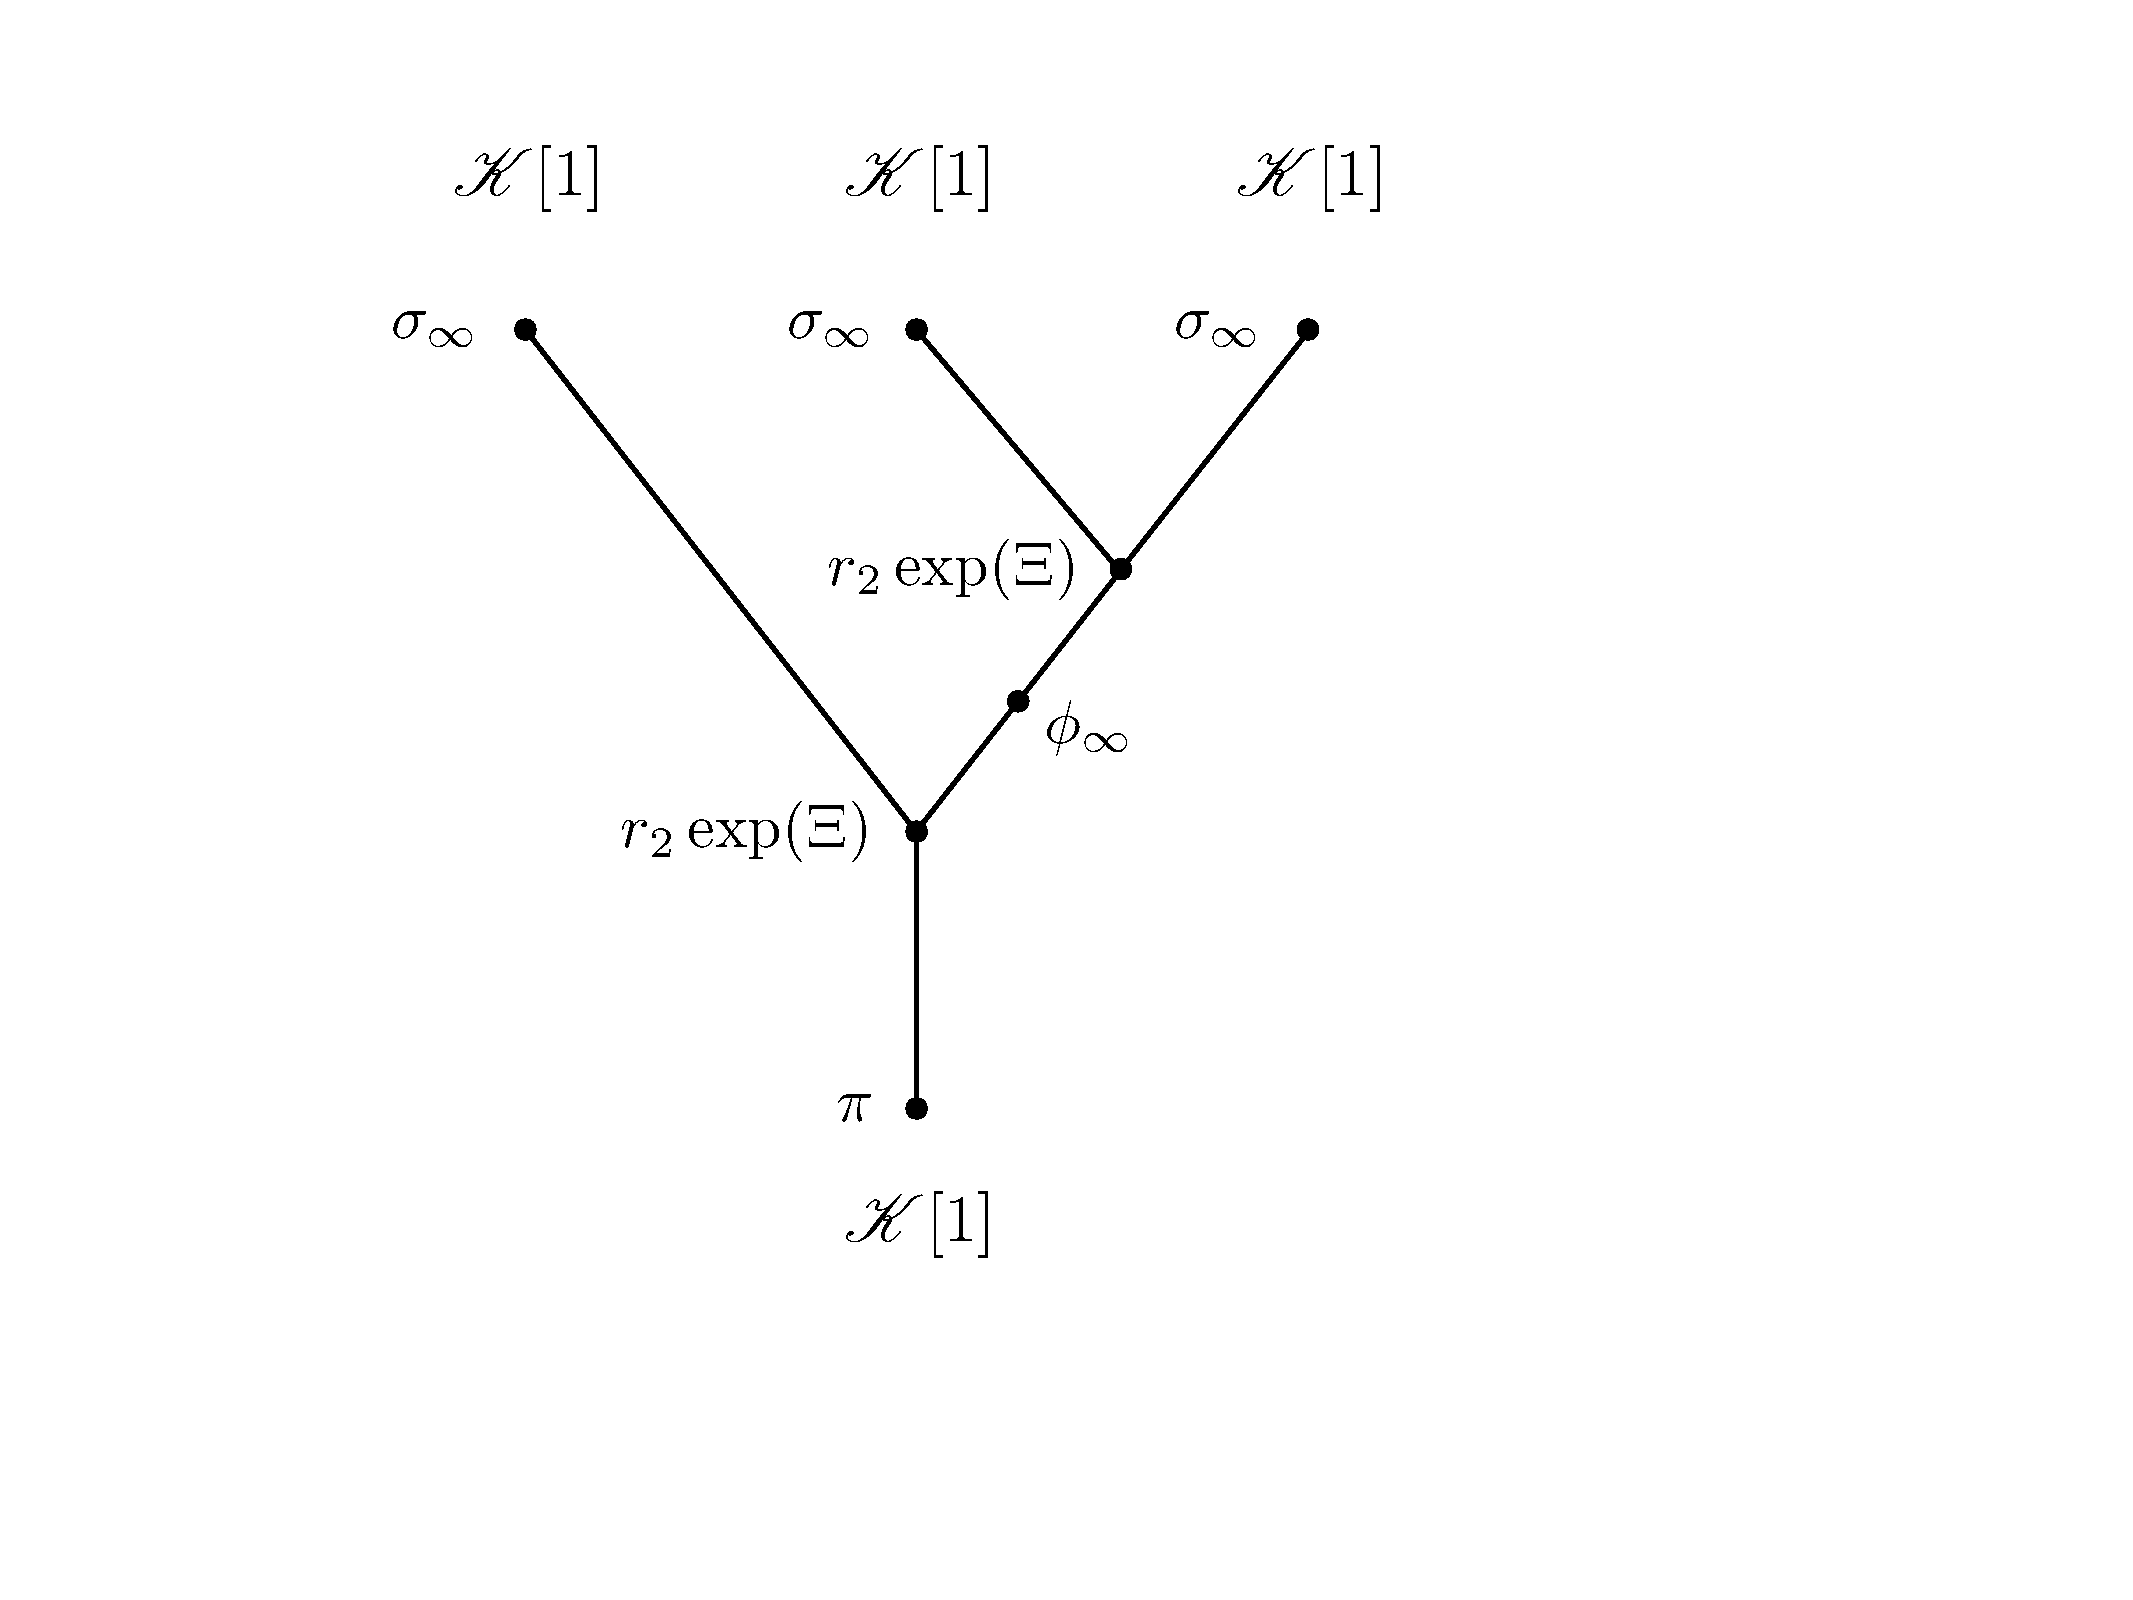
\includegraphics[scale=0.35]{dia12}
\end{tabular}
\end{center}
\end{lemma}
\begin{proof}
Fix a valid plane tree $T \in \cat{T}_k$ with only internal vertices of valency $3$. By definition $\rho_T$ is equal to $(-1)^{e_i(T)} \langle D \rangle$ where $\langle D \rangle$ is the branch denotation of the decoration $D$ of $A(T)$ given by assigning the same modules to edges and vertices, but
\begin{itemize}
\item $\Phi^{-1}: \KK[1] \lto \HH[1]$ to each input
\item $\Phi: \HH[1] \lto \KK[1]$ to the root
\item $\widehat{H}$ to internal edges
\item $r_2$ to internal vertices
\end{itemize}
Then by the definition of the branch denotation if the vertex adjacent to the root of $T$ has sub-branches $T_1,T_2$ with induced decorations $D_1,D_2$ then by Lemma \ref{lemma_12_2}
\begin{align*}
\langle D \rangle = \Phi \circ r_2 \circ ( \langle D \rangle_B \otimes \langle D_2 \rangle )\\
&= \pi \exp(-\delta) r_2( \langle D_1 \rangle \otimes \langle D_2 \rangle )\\
&= \pi r_2 \exp(\Xi) \circ ( \exp(-\delta) \otimes \exp(-\delta) ) \circ ( \langle D_1 \rangle \otimes \langle D_2 \rangle )\\
&= \pi r_2 \exp(\Xi)( \exp(-\delta) \langle D_1 \rangle \otimes \exp(-\delta) \langle D_2 \rangle )\,.
\end{align*}
Now each $T_i$ is either just a leaf, or begins with an internal edge, and in the former case
\[
\exp(-\delta) \langle D_i \rangle = \exp(-\delta) \Phi^{-1} = \sigma_\infty
\]
while in the latter case with $D'_i$ denoting the decoration of the sub-tree with that internal edge removed
\begin{align*}
\exp(-\delta) \langle D_i \rangle &= \exp(-\delta) \widehat{H} \langle D_i' \rangle\\
&= \exp(-\delta) \exp(\delta) \phi_\infty \exp(-\delta) \langle D_i' \rangle\\
&= \phi_\infty \exp(-\delta) \langle D_i' \rangle
\end{align*}
and so the claim holds by induction on the height of the tree.
\end{proof}


\bibliographystyle{amsalpha}
\providecommand{\bysame}{\leavevmode\hbox to3em{\hrulefill}\thinspace}
\providecommand{\href}[2]{#2}
\begin{thebibliography}{BHLS03}
  
\bibitem{lazaroiu}
C.~I.~Lazaroiu, \textsl{Generating the superpotential on a D-brane category: I}, [arXiv:hep-th/0610120].
  
\bibitem{murfet}
D.~Murfet, \textsl{Computing with cut systems}, \href{http://arxiv.org/abs/1402.4541}{[arXiv:1402.4541]}.

\bibitem{lgdual}
N.~Carqueville and D.~Murfet, \textsl{Adjunctions and defects in Landau-Ginzburg models}, Adv. Math. \textbf{289} (2016), 480--566.

\bibitem{dm1102.2957}
T.~Dyckerhoff and D.~Murfet, \textsl{Pushing forward matrix factorisations}, Duke Math. J. \textbf{162} (2013), 1249--1311.

\end{thebibliography}

\end{document}

